% !TeX TXS-program:compile = txs:///arara
% arara: lualatex: {shell: yes, synctex: no, interaction: batchmode}
% arara: pythontex: {rerun: always} if found('pytxcode', 'PYTHONTEX#py')
% arara: lualatex: {shell: yes, synctex: no, interaction: batchmode} if found('pytxcode', 'PYTHONTEX#py')
% arara: lualatex: {shell: yes, synctex: no, interaction: batchmode} if found('log', '(undefined references|Please rerun|Rerun to get)')

\documentclass[a4paper,11pt]{article}
\usepackage[revgoku]{cp-base}
\graphicspath{{./graphics/}}
\usepackage{ccicons}
\usepackage{standalone}
\makeatletter
	\@addtoreset{section}{part}
\makeatother
\usepackage{titletoc}
\addto{\captionsfrench}{%
	\renewcommand{\contentsname}{\vspace*{-20pt}}
}
\dottedcontents{part}[1.5em]{\color{OrangeRed}\large\sffamily\bfseries}{1.5em}{0.25em}[\addvspace{4pt}]
\dottedcontents{section}[3.8em]{\color{titrebleu}\sffamily\bfseries}{2.3em}{0.25em}[\addvspace{4pt}]
\dottedcontents{subsection}[7em]{\color{ForestGreen}\sffamily\bfseries}{3.2em}{0.25em}[\addvspace{4pt}]

%variables
\donnees[classe=1\up*{ère} 2M2,matiere={[SPÉ.MATHS]},typedoc=DOC~,numdoc=1,tailletitre=\LARGE]

%formatage
\author{Pierquet}
\title{\nomfichier}
\hypersetup{pdfauthor={Pierquet},pdftitle={\nomfichier},allbordercolors=white,pdfborder=0 0 0,pdfstartview=FitH}
%fancy
\lhead{\entete{\matiere}}
\chead{\entete{C. Pierquet}}
\rhead{\entete{\lycee{} - 2021/2022}}
\lfoot{\pied{\matiere}}
\cfoot{\ccbyncsa}
\rfoot{\pied{\numeropagetot}}
\fancypagestyle{entetedm}{\fancyhead[L]{\entete{\matiere{} À rendre avant le \ldots}}}
\fancypagestyle{enteteds}{\fancyhead[L]{\entete{Durée : \duree}}}
\fancypagestyle{entetedsa}{\fancyhead[L]{\entete{[SujetA] Durée : \duree}}}

%divers
\tikzset{tangent/.style={% https://tex.stackexchange.com/a/25940
		decoration={%
			markings,mark=at position #1 with{
				\coordinate (tangent point-\pgfkeysvalueof{/pgf/decoration/mark info/sequence number}) at (0pt,0pt);
				\coordinate (tangent unit vector-\pgfkeysvalueof{/pgf/decoration/mark info/sequence number}) at (1,0pt);
				\coordinate (tangent orthogonal unit vector-\pgfkeysvalueof{/pgf/decoration/mark info/sequence number}) at (0pt,1);}
		},
		postaction=decorate},
	use tangent/.style={shift=(tangent point-#1),%
		x=(tangent unit vector-#1),
		y=(tangent orthogonal unit vector-#1)
	},
	use tangent/.default=1}
\usepackage{setspace}
\usepackage{epsdice}
\tcbset{cartepoker/.style={%
		fontupper={\vphantom{pf}\scriptsize\sffamily},colback=white,nobeforeafter,%
		box align=base,boxsep=0pt,enhanced,width=16pt,tcbox width=forced center,%
		boxrule=0.7pt,left=2pt,right=2pt,top=0pt,bottom=0pt
	}
}
% Commande qui trace la grille entre (xmin,ymin) et (xmax,ymax)
\newcommand {\grille}
{\draw[help lines] (\xmin,\ymin) grid (\xmax,\ymax);}
% Commande \axes
\newcommand {\axes} {
	\draw[thick,->,>=stealth'] (\xmin,0) -- (\xmax,0);
	\draw[thick,->,>=stealth'] (0,\ymin) -- (0,\ymax);
}
% Commande qui limite l’affichage à (xmin,ymin) et (xmax,ymax)
\newcommand {\fenetre}
{\clip (\xmin,\ymin) rectangle (\xmax,\ymax);}
%cercletrigo
\newcommand\cercletrigo{%
	\draw (0,0) circle[radius=2] ;
	\draw (-2.25,0) -- (2.25,0) ;
	\draw (0,-2.25) -- (0,2.25) ;
	\draw[->,>=stealth'] (0,0) -- (2,0) ;
	\draw[->,>=stealth'] (0,0) -- (0,2) ;
	%\draw (0,0) node[below left] {$O$} ;
}

\begin{document}

\pagestyle{fancy}

\part*{Spécialité Mathématiques en classe de Première - Évaluations}

\tableofcontents

\clearpage

% !TeX TXS-program:compile = txs:///lualatex

\documentclass[a4paper,11pt]{article}
\usepackage[]{cp-base} %avec options possibles parmi breakable (tcbox), sujetl (exos),  (pour faire "comme avant"), etc...
\graphicspath{{./graphics/}}
%variables
\donnees[%
	classe=1\up{ère} 2M2,
	matiere={[SPÉ.MATHS]},
	typedoc=DM,
	numdoc=1,
	titre={Mise en boîte},
	mois=Septembre,
	annee=2021,
	]

%formatage
\author{Pierquet}
\title{\nomfichier}
\hypersetup{pdfauthor={Pierquet},pdftitle={\nomfichier},allbordercolors=white,pdfborder=0 0 0,pdfstartview=FitH}
%divers
\lhead{\entete{\matiere}}
\chead{\entete{\lycee}}
\rhead{\entete{\classe{} - \mois{} \annee}}
\lfoot{\pied{\matiere}}
\cfoot{\logolycee{}}
\rfoot{\pied{\numeropagetot}}
\fancypagestyle{entetedm}{\fancyhead[L]{\entete{\matiere{} À rendre avant le \ldots}}}

\begin{document}
	
\pagestyle{fancy}

\thispagestyle{entetedm}
	
\part{DM01 - Mise en boîte}

\medskip

On dispose d’un carré en métal de 40 cm de côté. Pour construire une boîte parallélépipédique, on retire à chaque coin un carré de côté $x$ cm et on relève les bords par pliage (voir figure).
\begin{center}
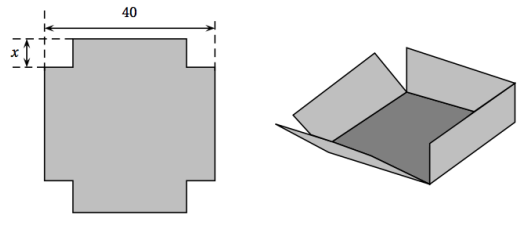
\includegraphics[scale=0.7]{graphics/dm05_patron}
\end{center}

On note $f$ la fonction qui au nombre $x$ associe le volume $f(x)$ en cm$^3$ de la boîte obtenue.

\begin{enumerate}
	\item
	\begin{enumerate}
		\item Déterminer l'ensemble de définition (autrement dit l'ensemble des valeurs de $x$ pour lesquelles le volume $f(x)$ existe), noté $I$, de la fonction $f$.
		\item Calculer $f(5)$ et interpréter le sens concret de ce résultat.
	\end{enumerate}
	\item Déterminer l'expression de $f(x)$ en fonction de $x$ pour $x \in I$.
	\item À l'aide de la trame de graphique suivant pour lequel les unités sont à préciser, tracer la courbe représentative de la fonction $f$ pour $x \in I$.
		\begin{center}
			\tunits{0.75}{0.0015}
			\tdefgrille{0}{21}{1}{1}{0}{5000}{500}{500}
			\tikzset{pointilles/.style={densely dashed,line width=1.5pt}}
			\begin{tikzpicture}[x=\xunit cm,y=\yunit cm]
				%AXES/GRILLE
				\tgrillep[line width=0.4pt,orange!50]
				\draw[line width=0.4pt,orange!50] (0,5000) -- (21,5000) ;
				\axestikz \axextikz*{0,1,...,20} \axeytikz*{0,500,...,4500}
			\end{tikzpicture}
		\end{center}
	\item On répondra aux questions suivantes à l’aide de la représentation graphique de $f$ avec la précision permise par ce graphique.
	
	\textit{On laissera apparents sur le graphique les pointillés utiles pour la lecture graphique.}
	\begin{enumerate}
		\item Donner les éventuels antécédents de 2\,500 par $f$ et interpréter le résultat.
		\item Pour quelles valeurs de $x$ le volume de la boîte est-il inférieur à 2\,000 cm$^3$ ?
		\item Quel volume maximum peut-on obtenir en fabriquant une boîte comme ceci ? Pour quelle valeur de $x$ ce volume maximal est-il atteint ?
	\end{enumerate}
	\item
	\begin{enumerate}
		\item Déterminer graphiquement les solutions de $f(x)=\num{3000}$.
		\item Déterminer, par tabulations successives, une valeur approchée à $10^{-2}$ près de(s) solution(s) de l'équation $f(x)=\num{3000}$.
	\end{enumerate} 
\end{enumerate}

\end{document}

\clearpage

% !TeX TXS-program:compile = txs:///lualatex

\documentclass[a4paper,11pt]{article}
\usepackage[]{cp-base} %avec options possibles parmi breakable (tcbox), sujetl (exos),  (pour faire "comme avant"), etc...
\graphicspath{{./graphics/}}
%variables
\donnees[%
	classe=1\up{ère} 2M2,
	matiere={[SPÉ.MATHS]},
	typedoc=DM,
	numdoc=02,
	mois=Septembre,
	annee=2021,
	titre={Étude de bénéfices}
	]
	
%formatage
\author{Pierquet}
\title{\nomfichier}
\hypersetup{pdfauthor={Pierquet},pdftitle={\nomfichier},allbordercolors=white,pdfborder=0 0 0,pdfstartview=FitH}
%divers
\lhead{\entete{\matiere}}
\chead{\entete{\lycee}}
\rhead{\entete{\classe{} - \mois{} \annee}}
%\rhead{\entete{\classe{} - Chapitre }}
\lfoot{\pied{\matiere}}
\cfoot{\logolycee{}}
\rfoot{\pied{\numeropagetot}}
\fancypagestyle{entetedm}{\fancyhead[L]{\entete{\matiere{} À rendre avant le\ldots}}}

\begin{document}

\pagestyle{fancy}

\thispagestyle{entetedm}

\part{DM02 - Étude de bénéfices}

\medskip

Une entreprise fabrique des petits meubles. Pour des raisons de stockage, la production mensuelle $x$ est comprise entre 0 et 800 unités.

Le coût total de fabrication mensuel, exprimé en euros, est donné par la fonction $C$ définie sur $\intervFF{0}{800}$ par :\[ C(x)=0,05x^2+20x+1\,250. \]
On a tracé ci-dessous la courbe de la fonction $C$ ainsi que la droite $\mathcallig{R}$ représentant la fonction recette, le tout dans un repère orthogonal.

\begin{center}
	\tunits{0.18}{0.18}
	\tdefgrille{0}{85}{5}{5}{0}{50}{50}{5}
	\begin{tikzpicture}[x=\xunit cm,y=\yunit cm]
		%AXES & GRILLES
		\tgrilles[orange!50,line width=0.4pt,densely dashed] 
		\axestikz
		\foreach \x in {0,5,...,80}
			\FPeval{calx}{clip(\x*10)}
			\draw[line width=1.25pt] (\x,4pt) -- (\x,-4pt) node[below] {\num{\calx}} ;
		%\axextikz{0,50,...,800} ;
		\foreach \y in {0,5,...,45}
			\FPeval{caly}{clip(\y*1000)}
			\draw[line width=1.25pt] (4pt,\y) -- (-4pt,\y) node[left] {\num{\caly}} ;
		%COURBE
		\draw[line width=1.25pt,red,domain=0:80] plot (\x,{0.005*\x*\x+0.20*\x+1.250}) ;
		\draw[line width=1.25pt,blue,domain=0:80] plot (\x,{0.475*\x}) ;
		\draw[darkgray,fill=darkgray] (65,30.875) circle(3pt) ;
		\draw (65,30.875) node[below right] {$(650\,;\,30\,875)$} ;
	\end{tikzpicture}
\end{center}

\begin{enumerate}
	\item À l’aide du graphique, déterminer le prix de vente exact de chaque meuble.
	\item Calculer la recette, puis le bénéfice correspondant à 150 meubles fabriqués et vendus.
	\item Graphiquement, sur quel intervalle l’entreprise réalise-t-elle des bénéfices ? Justifier.
	\item 
	\begin{enumerate}
		\item Donner la recette mensuelle $R(x)$, exprimée en euros, correspondant à $x$ meubles vendus.
		\item En déduire le bénéfice mensuel $B(x)$, exprimé en euros, correspondant à $x$ meubles fabriqués et vendus.
	\end{enumerate}
	\item
	\begin{enumerate}
		\item Déterminer, en détaillant, la forme canonique de la fonction $B$.
		\item Déterminer, en justifiant, le nombre de meubles à fabriquer et à vendre pour que le bénéfice soit maximal. Préciser la valeur de ce bénéfice maximal.
	\end{enumerate}
	\item 
	\begin{enumerate}
		\item Résoudre l'équation $B(x)=0$.
		\item Déterminer la forme factorisée de $B(x)$.
		
		\textbf{NB} : On pourrait ainsi retrouver, par calculs, le résultat de la question \ptno{3} !
	\end{enumerate}
	\item Déterminer, par la méthode de votre choix, les quantités de meubles à fabriquer et à vendre pour que le bénéfice soit de :
	\begin{enumerate}
		\item $-1\,250$\,€ ;
		\item 1\,000\,€.
	\end{enumerate}
\end{enumerate}

\end{document}

\clearpage

% !TeX TXS-program:compile = txs:///lualatex

\documentclass[a4paper,11pt]{article}
\usepackage[revgoku]{cp-base} %avec options possibles parmi breakable (tcbox), sujetl (exos),  (pour faire "comme avant"), etc...
\graphicspath{{./graphics/}}
%variables
\donnees[%
	classe=1\up{ère} 2M2,
	matiere={[SPÉ.MATHS]},
	mois=Novembre,
	annee=2021,
	typedoc=DM,
	numdoc=03,
	titre={Second degré, suites}
	]

%formatage
\author{Pierquet}
\title{\nomfichier}
\hypersetup{%
	pdfauthor={Pierquet},pdftitle={\nomfichier},allbordercolors=white,pdfborder=0 0 0,pdfstartview=FitH}
%divers
\lhead{\entete{\matiere}}
\chead{\entete{\lycee}}
\rhead{\entete{\classe{} - \mois{} \annee}}
%\rhead{\entete{\classe{} - Chapitre }}
\lfoot{\pied{\matiere}}
\cfoot{\logolycee{}}
\rfoot{\pied{\numeropagetot}}
\fancypagestyle{entetedm}{\fancyhead[L]{\entete{\matiere{} À rendre avant le\ldots}}}

\begin{document}

\pagestyle{fancy}

\thispagestyle{entetedm}

\part{DM03 - Second degré, suites}

\medskip

\exonum{}

\smallskip

Une entreprise fabriquant des montures de lunettes veut créer un nouveau modèle. Son prix est à fixer entre 150\,€ et 800\,€. Une étude de marché a permis d’estimer que le nombre de personnes disposées à acheter ce modèle au prix unitaire de $x$ euros est $N(x)=-0,7x+588$ pour $x \in \intervFF{150}{800}$.
\begin{enumerate}
	\item 
	\begin{enumerate}
		\item Justifier que le chiffre d’affaires $R(x)$, en €, pour un prix $x$ est $R(x)=-0,7x^2+588x$ pour $x \in \intervFF{150}{800}$.
		\item Pour ce modèle de lunettes, les frais fixes de fabrication sont de 10\,000€, les frais variables de fabrication sont de 150\,€ par monture. Le coût total est donné par la formule $C(x)=10\,000+150 \times N(x)$.
		
		Justifier que $C(x)=-105x+98\,200$.
		\item En déduire le bénéfice algébrique $B(x)$ dégagé par la vente de montures au prix unitaire de $x$\,€.
	\end{enumerate}
	\item 
	\begin{enumerate}
		\item Résoudre l’équation $B(x)=0$ (arrondir au centime près).
		\item En déduire les solutions de l'inéquation $B(x) \pg 0$. Interpréter le résultat.
	\end{enumerate}
	\item Déterminer, en justifiant, le bénéfice maximal ainsi que le prix de vente (arrondi au centième) le garantissant.
\end{enumerate}

\medskip

\exonum{}

\smallskip

Dans cet exercice, on s'intéresse à la modélisation de l'évolution de la population mondiale à partir de 1800, qui est estimée à 1\,000 millions d'individus en 1800.

\smallskip

\textbf{Partie A - Un premier modèle}

\smallskip

On suppose que la population mondiale augmente (de manière régulière) de 41,1 millions d'individus tous les 5 ans. On note $\suiten$ la suite modélisant la population mondiale, en millions, l'année $1800+5n$, avec $u_0=1\,000$.
%
\begin{enumerate}
	\item Calculer $u_1$ et $u_2$. Interpréter les résultats dans le contexte de l'exercice.
	\item Exprimer $u_{n+1}$ en fonction de $u_n$.
	\item 
	\begin{enumerate}
		\item À l'aide de la calculatrice, déterminer une estimation de la population mondiale en 1930.
		\item Faire de même pour la population mondiale en 2020. Ce résultat semble-t-il être cohérent avec les 7\,700 millions d'individus en 2019 ?
	\end{enumerate}
\end{enumerate}

\textbf{Partie B - Un second modèle}

\smallskip

On suppose de ce fait que le modèle précédent n'est valable que jusque 1930, année pour laquelle la population mondiale était d'environ 2\,070 millions d'individus. À partir de 1930, on considère que la population mondiale augmente (de manière régulière) de 8,17\,\% tous les 5 ans. On note $\suiten[v]$ la suite modélisant la population mondiale, en millions, l'année $1930+5n$, avec en particulier $v_0=2\,070$.
%
\begin{enumerate}
	\item Calculer $v_1$ et $v_2$. Interpréter les résultats dans le contexte de l'exercice.
	\item Exprimer $v_{n+1}$ en fonction de $v_n$.
	\item 
	\begin{enumerate}
		\item À l'aide de la calculatrice, déterminer une estimation de la population mondiale en 2000.
		\item Faire de même pour la population mondiale en 2020. Ce résultat semble-t-il de nouveau être cohérent ?
	\end{enumerate}
\end{enumerate}

\textbf{Partie C - Utilisation d'un tableur}

\smallskip

On souhaite, sur un tableur, calculer les termes successifs des suites $\suiten$ et $\suiten[v]$ sur leur domaine de validité.
%
\begin{center}
	\begin{tikzpicture}
		\tableur*[4]{A/2cm,B/2cm,C/2cm,D/0.75cm,E/2cm,F/2cm,G/2cm}
		%L1
		\celtxt[c]{A}{1}{Année}
		\celtxt[c]{B}{1}{n}
		\celtxt[c]{C}{1}{u\_n}
		\celtxt[c]{E}{1}{Année}
		\celtxt[c]{F}{1}{n}
		\celtxt[c]{G}{1}{v\_n}
		%L2
		\celtxt[c]{A}{2}{1800}
		\celtxt[c]{B}{2}{0}
		\celtxt[c]{C}{2}{1000}
		\celtxt[c]{E}{2}{1930}
		\celtxt[c]{F}{2}{0}
		\celtxt[c]{G}{2}{2070}
		%Les valeurs de n
		\celtxt[c]{B}{3}{1}
		\celtxt[c]{B}{4}{2}
		%\celtxt[c]{B}{5}{3}
%		\celtxt[c]{B}{6}{4}
		\celtxt[c]{F}{3}{1}
		\celtxt[c]{F}{4}{2}
		%\celtxt[c]{F}{5}{3}
%		\celtxt[c]{F}{6}{4}
	\end{tikzpicture}
\end{center}
%
\begin{enumerate}
	\item Quelles formules, à recopier, doit-on rentrer dans les cellules \csheet{A3} et \csheet{E3} afin d'afficher les années d'étude ?
	\item Quelles formules, à recopier, doit-on rentrer en \csheet{C3} et \csheet{G3} afin d'afficher l'estimation de la population ?
\end{enumerate}

\end{document}

\clearpage

% !TeX TXS-program:compile = txs:///pythonlua

\documentclass[a4paper,11pt]{article}
\usepackage[pythontex,revgoku]{cp-base}
\graphicspath{{./graphics/}}
%variables
\donnees[%
	classe=1\up{ère} 2M2,
	matiere={[SPÉ.MATHS]},
	mois=Décembre,
	annee=2021,
	typedoc=DM,
	numdoc=04,
	titre={Second degré en situation(s)}
	]

%formatage
\author{Pierquet}
\title{\nomfichier}
\hypersetup{pdfauthor={Pierquet},pdftitle={\nomfichier},allbordercolors=white,pdfborder=0 0 0,pdfstartview=FitH}
%divers
\lhead{\entete{\matiere}}
\chead{\entete{\lycee}}
\rhead{\entete{\classe{} - \mois{} \annee}}
\lfoot{\pied{\matiere}}
\cfoot{\logolycee{}}
\rfoot{\pied{\numeropagetot}}
\fancypagestyle{entetedm}{\fancyhead[L]{\entete{\matiere{} À rendre avant le\ldots}}}

\begin{document}

\pagestyle{fancy}

\thispagestyle{entetedm}

\part{DM04 - Second degré en situation(s)}

\smallskip

\exotitre{Exercice 1 - En SES}

\medskip

Une entreprise fabrique des composants électroniques. Sa production mensuelle est inférieure à 12\,000 articles.

Le coût total mensuel, en milliers d’euros, pour produire $x$ milliers d’articles est modélisé par la fonction C définie sur $\intervFF{0}{12}$ par $C(x) = 0,6x^2 - 0,62x + 18,24$. Chaque article fabriqué est vendu au prix unitaire de 7\,€.

\begin{enumerate}
	\item L’entreprise a produit et vendu 4\,000 articles en mai 2018 et 6\,500 articles en juin 2018.
	
	Le bénéfice a-t-il été plus important au mois de juin ?
	\item On note $R(x)$ le montant, en milliers d’euros, de la recette mensuelle pour $x$ milliers d’articles vendus.
	
	Exprimer $R(x)$ en fonction de $x$.
	\item Tracer soigneusement, dans le repère donné en annexe (les unités sont à préciser), les courbes représentatives $\mathscr{C}$ et $\mathscr{R}$ des fonctions C et R. 
	\item Avec la précision permise par le graphique, déterminer :
	\begin{enumerate}
		\item l’intervalle dans lequel doit se situer $x$ pour que le bénéfice mensuel réalisé soit positif ;
		\item la valeur de $x$ pour laquelle le bénéfice mensuel est maximal.
	\end{enumerate}
	\item On note $B(x)$ le bénéfice mensuel, en milliers d’euros, réalisé lorsque l’entreprise produit et vend $x$ milliers d’articles.
	\begin{enumerate}
		\item Vérifier que, pour tout $x \in \intervFF{0}{12}$, on a $B(x) = -0,6x^2 + 7,62x - 18,24$.
		\item Étudier le signe de $B(x)$ et les variations de la fonction B sur $\intervFF{0}{12}$.
	\end{enumerate}
	\item En déduire le nombre d’articles que l’entreprise doit produire pour réaliser un bénéfice mensuel :
	\begin{enumerate}
		\item positif ; 
		\item maximal.
	\end{enumerate}
\end{enumerate}

\medskip

\exotitre{Exercice 2 - En programmation}

\medskip

On considère la fonction suivante en \calgpython{} qui fait intervenir une fonction $f$ polynôme du second degré :

\begin{tcpythoncode}[10cm]
	\begin{pyverbatim}[][fontsize=\footnotesize,numbers=left,numbersep=10pt]
		def point_f(x,y) :
			if y == 3*x**2-x-2 :
				return True
			else :
				return False
	\end{pyverbatim}
\end{tcpythoncode}

\begin{enumerate}
	\item Donner une expression de $f(x)$.
	\item On appelle la fonction \cpy{point\_f} avec les paramètres \cpy{x=-1/3} et \cpy{y=-29/3}. Que renvoie-t-elle ?
	\item On appelle la fonction \cpy{point\_f} avec les paramètres \cpy{x=-1} et \cpy{y=2}. Que renvoie-t-elle ?
	\item Préciser le rôle de cette fonction en \calgpython.
	\item Déterminer la forme factorisée de $f$.
	\item 
	\begin{enumerate}
		\item L’utilisateur a choisi \cpy{0} pour \cpy{y} et la fonction en \calgpython{} a renvoyé le booléen \cpy{True}. Quelle(s) valeur(s) de \cpy{x} l’utilisateur a-t-il pu choisir ? Justifier.
		\item L’utilisateur a choisi \cpy{-2} pour \cpy{y} et la fonction en \calgpython{} a renvoyé le booléen \cpy{True}. Quelle(s) valeur(s) de \cpy{x} l’utilisateur a-t-il pu choisir ? Justifier.
	\end{enumerate}
\end{enumerate}

\newpage

\exotitre{Exercice 1 - Annexe}

\medskip

\begin{center}
	\tunits{1.5}{0.2}
	\tdefgrille{0}{12}{1}{0.5}{0}{100}{5}{2.5}
	\begin{tikzpicture}[x=\xunit cm,y=\yunit cm]
		\tgrilles[line width=0.3pt,lightgray] ;
		\tgrillep[line width=0.6pt,gray!50] ;
		\axestikz* ;
		\foreach \x in {0,1,...,11} \draw[line width=1.25pt] (\x,4pt) -- (\x,-4pt) ;
		\foreach \y in {0,5,...,90} \draw[line width=1.25pt] (4pt,\y) -- (-4pt,\y) ;
		%\draw[line width=1.5pt,red,domain=0:12,samples=250] plot (\x,{0.6*\x*\x-0.62*\x+18.24}) ;
		%\draw[line width=1.5pt,blue,domain=0:12,samples=250] plot (\x,{7*\x}) ;
	\end{tikzpicture}
\end{center}


\end{document}

\clearpage

% !TeX TXS-program:compile = txs:///pythonlualatex

\documentclass[a4paper,11pt]{article}
\usepackage[pythontex,revgoku]{cp-base}
\graphicspath{{./graphics/}}
%variables
\donnees[classe=1\up{ère} 2M2,matiere={[SPÉ.MATHS]},mois=Janvier,annee=2022,typedoc=DM,numdoc=5,titre={Probabilités conditionnelles}]

%formatage
\author{Pierquet}
\title{\nomfichier}
\hypersetup{pdfauthor={Pierquet},pdftitle={\nomfichier},allbordercolors=white,pdfborder=0 0 0,pdfstartview=FitH}
%divers
\lhead{\entete{\matiere}}
\chead{\entete{\lycee}}
\rhead{\entete{\classe{} - \mois{} \annee}}
\lfoot{\pied{\matiere}}
\cfoot{\logolycee{}}
\rfoot{\pied{\numeropagetot}}
\fancypagestyle{entetedm}{\fancyhead[L]{\entete{\matiere{} À rendre avant le\ldots}}}

\begin{document}

\pagestyle{fancy}

\thispagestyle{entetedm}

\setcounter{numexos}{0}

\part{DM05 - Probabilités conditionnelles}%barbazo exo37p296

\smallskip

\exonum{2}

\medskip

Une entreprise conditionne du sucre blanc provenant de deux exploitations U et V en paquets de 1 kg et de différentes qualités. Le sucre extra fin est conditionné séparément dans des paquets portant le label « extra fin ».

\smallskip

Les résultats seront arrondis, si nécessaire, au millième.

\smallskip

On sait que 3\,\% du sucre provenant de l’exploitation U est extra fin et 5\,\% du sucre provenant de l’exploitation V est extra fin. On prélève au hasard un paquet de sucre dans la production de l’entreprise et, dans un souci de traçabilité, on s’intéresse à la provenance de ce paquet.

\smallskip

On considère les évènements suivants :
%
\begin{itemize}
	\item U : « Le paquet contient du sucre provenant de l’exploitation U » ;
	\item V : « Le paquet contient du sucre provenant de l’exploitation V » ;
	\item E : « Le paquet porte le label "extra fin" ».
\end{itemize}
%
\begin{enumerate}
	\item Dans cette question, on admet que l’entreprise fabrique 30\,\% de ses paquets avec du sucre provenant de l’exploitation U et les autres avec du sucre provenant de l’exploitation V, sans mélanger les sucres des deux exploitations.
	\begin{enumerate}
		\item Construire un arbre pondéré représentant la situation.
		\item Quelle est la probabilité que le paquet prélevé porte le label « extra fin » ? 
		\item Sachant qu’un paquet porte le label « extra fin », quelle est la probabilité que le sucre qu’il contient provienne de l’exploitation U ? 
	\end{enumerate}
	\item L’entreprise souhaite modifier son approvisionnement auprès des deux exploitations afin que, parmi les paquets portant le label « extra fin », 30\,\% d’entre eux contiennent du sucre provenant de l’exploitation U. On cherche à déterminer comment elle doit s’approvisionner auprès des 
	exploitations U et V.
	
	On ne connaît donc pas, dans cette question, $P(U)$, et on va noter $P(U)=x$.
	\begin{enumerate}
		\item Construire, à l'aide de $x$, un arbre de pondéré représentant la situation.
		\item Déterminer, en détaillant la démarche, les valeurs de $P(U)$ et de $P(V)$.
	\end{enumerate}
\end{enumerate}

\medskip

\exonum{2}

\medskip

Une urne contient \textcolor{ForestGreen}{cinq bulletins verts} et {\blue trois bulletins bleus}. Lucien a écrit le script \calgpython{} d’une fonction \cpy{tirage}.

\begin{envpython}[12cm]
	from random import randint
	def tirage():
		tirage=[]
		for i in range(2):
			if randint(1,8)<=3:
				tirage.append("bleu")
			else :
				tirage.append("vert")
		return(tirage)
\end{envpython}

\begin{enumerate}
	\item Que renvoie cette fonction ?
	\item Quelle est la probabilité que cette fonction renvoie \cpy{['bleu','bleu']} ?
	\item[Bonus] Modifier le script de la fonction \cpy{tirage} pour qu’elle renvoie le nombre de bulletins bleus obtenus lors de deux tirages avec remise dans l’urne.
\end{enumerate}

\end{document}

\clearpage

% !TeX TXS-program:compile = txs:///lualatex

\documentclass[a4paper,11pt]{article}
\usepackage[revgoku]{cp-base}
\graphicspath{{./graphics/}}
%variables
\donnees[%
	classe=1\up{ère} 2M2,
	matiere={[SPÉ.MATHS]},
	mois=Janvier,
	annee=2022,
	typedoc=DM,
	numdoc=06,
	titre={Probabilités (v2)}
	]

%formatage
\author{Pierquet}
\title{\nomfichier}
\hypersetup{pdfauthor={Pierquet},pdftitle={\nomfichier},allbordercolors=white,pdfborder=0 0 0,pdfstartview=FitH}
%divers
\lhead{\entete{\matiere}}
\chead{\entete{\lycee}}
\rhead{\entete{\classe{} - \mois{} \annee}}
\lfoot{\pied{\matiere}}
\cfoot{\logolycee{}}
\rfoot{\pied{\numeropagetot}}
\fancypagestyle{entetedm}{\fancyhead[L]{\entete{\matiere{} À rendre avant le\ldots}}}

\begin{document}

\pagestyle{fancy}

\thispagestyle{entetedm}

\setcounter{numexos}{0}

\part{DM06 - Probabilités (v2)}

\smallskip

\exonum{}

\medskip

Lors d’une course cyclosportive, 70\,\% des participants sont licenciés dans un club, les autres ne sont pas licenciés. Aucun participant n’abandonne la course.

Parmi les licenciés, 66\,\% font le parcours en moins de 5 heures ; les autres en plus de 5 heures.

Parmi les non licenciés, 83\,\% font le parcours en plus de 5 heures; les autres en moins de 5 heures.

On interroge au hasard un cycliste ayant participé à cette course et on note :
%
\begin{itemize}
	\item L l’évènement « le cycliste est licencié dans un club » et $\overline{L}$ son évènement contraire,
	\item M l’évènement « le cycliste fait le parcours en moins de 5 heures » et $\overline{M}$ son évènement contraire.
\end{itemize}
%
\begin{enumerate}
	\item À l’aide des données de l’énoncé préciser les valeurs de $P(L)$, $P_L(M)$ et $P_L \big( \overline{M} \big)$.
	\item Construire un arbre pondéré suivant représentant la situation.
	\item Calculer la proba. que le cycliste interrogé soit licencié dans un club et ait réalisé le parcours en moins de 5~h.
	\item Justifier que $P(M) = 0,513$.
	\item Un organisateur affirme qu’au moins 90\,\% des cyclistes ayant fait le parcours en moins de 5 heures sont licenciés dans un club. A-t-il raison ? Justifier la réponse.
	\item Un journaliste interroge indépendamment trois cyclistes au hasard. On suppose le nombre de cyclistes suffisamment important pour assimiler le choix de trois cyclistes à un tirage aléatoire avec remise.
	
	Calculer la probabilité qu’exactement deux des trois cyclistes aient réalisé le parcours en moins de 5~h.
\end{enumerate}

\smallskip

\exonum{}

\medskip

Un concessionnaire automobile vend deux versions de voitures pour une marque donnée: routière ou break. Pour chaque version il existe deux motorisations : essence ou diesel. Le concessionnaire choisit au hasard un client ayant déjà acheté une voiture. On note : 
%
\begin{itemize}
	\item $R$ l'évènement: \og la voiture achetée est une routière \fg{} ;
	\item $B$ l'évènement: \og la voiture achetée est une break \fg{}; 
	\item $E$ l'évènement : \og la voiture est achetée avec une motorisation essence \fg{} ;
	\item $D$ l'évènement : \og la voiture est achetée avec une motorisation diesel \fg. 
\end{itemize}
%
On sait, de plus, que :
%
\begin{itemize}
	\item[$\bullet~$]  65\,\% des clients achètent une voiture routière. 
	\item[$\bullet~$] Lorsqu'un client achète une voiture break, il choisit dans 85\:\% des cas la motorisation diesel. 
	\item[$\bullet~$] 27,3\,\% des clients achètent une voiture routière avec une motorisation diesel.
\end{itemize}
%
\begin{enumerate}
	\item Quelle est la probabilité $p(R)$ de l'événement $R$ ? 
	\item 
	\begin{enumerate}
		\item Construire l'arbre de probabilité (qui sera complété petit à petit). 
		\item Démontrer que $p_{R}(D) = 0,42$.
		\item Calculer $p(D)$. 
	\end{enumerate}
	\item Lorsque le concessionnaire a choisi au hasard un client, on s'intéresse au prix de vente (en milliers d'euros) de la voiture achetée. Compléter le tableau suivant :
	\begin{center}
		\setlength{\arrayrulewidth}{1.1pt}
		\renewcommand{\arraystretch}{1.05}
		\textsf{\begin{tabularx}{0.9\linewidth}{|l|*{4}{Y|}}
			\hline
			Version &\multicolumn{2}{c|}{Routière} &\multicolumn{2}{c|}{Break} \\ \hline
			Motorisation &Essence&Diesel &Essence &Diesel \\ \hline
			$\mathsf{x_{i}}$ : prix de vente (en milliers d'€) &15 &18 &17 &20\\ \hline 
			$\mathsf{p_{i}}$ : probabilité&& 0,273&&\\ \hline
		\end{tabularx} }
	\end{center}
	Calculer le prix de vente moyen des voitures achetées.
\end{enumerate}

\end{document}

\clearpage

% !TeX TXS-program:compile = txs:///lualatex

\documentclass[a4paper,11pt]{article}
\usepackage[revgoku]{cp-base}
\graphicspath{{./graphics/}}
%variables
\donnees[%
	classe=1\up{ère} 2M2,
	matiere={[SPÉ.MATHS]},
	mois=Février,
	annee=2022,
	typedoc=DM,
	numdoc=07,
	]

%formatage
\author{Pierquet}
\title{\nomfichier}
\hypersetup{pdfauthor={Pierquet},pdftitle={\nomfichier},allbordercolors=white,pdfborder=0 0 0,pdfstartview=FitH}
%divers
\lhead{\entete{\matiere}}
\chead{\entete{\lycee}}
\rhead{\entete{\classe{} - \mois{} \annee}}
%\rhead{\entete{\classe{} - Chapitre }}
\lfoot{\pied{\matiere}}
\cfoot{\logolycee{}}
\rfoot{\pied{\numeropagetot}}
\fancypagestyle{entetedm}{\fancyhead[L]{\entete{\matiere{} À rendre avant le\ldots}}}

\begin{document}

\pagestyle{fancy}

\thispagestyle{entetedm}

\setcounter{numexos}{0}

\part{DM07 - Dérivation locale (facultatif)}

\medskip

\exonum{3}

\medskip

Soit une fonction $f$ définie et dérivable sur $\R$.

Sa courbe représentative {\red $\mathscr{C}_f$} passe par les points {\blue $A(-4\,;\,11)$}, \textcolor{ForestGreen}{$B(2\,;\,4)$} et \textcolor{purple}{$C(6\,;\,2)$}.

Les nombres dérivés de $f$ en $-4$, en $2$ et en $6$ sont respectivement égaux à $-\frac{1}{5}$, à $\frac{1}{5}$ et à $0,465$.

\smallskip

On appelle {\blue $T_A$}, \textcolor{ForestGreen}{$T_B$} et \textcolor{purple}{$T_C$} les tangentes à {\red $\mathscr{C}_f$} respectivement en {\blue $A$}, en \textcolor{ForestGreen}{$B$} et en \textcolor{purple}{$C$}.

\begin{center}
	\tunits{0.45}{0.45}
	\tdefgrille{-10}{14}{2}{2}{-4}{12}{2}{2}
	\begin{tikzpicture}[x=\xunit cm,y=\yunit cm]
		%grilles & axes
		\tgrilles[line width=0.3pt,lightgray!50] ;
		\tgrillep[line width=0.6pt,lightgray!50] ;
		\axestikz* ;
		\axextikz[]{-10,-8,...,12} ;
		\axeytikz[]{-4,-2,...,10} ;
		\clip (\xmin,\ymin) rectangle (\xmax,\ymax) ;
		%splines
		\def\liste{-6/-4/15§-4/11/-0.2§0/4/-0.5§2/4/0.2§6/2/0.465§8/12/8}
		%splines ?
		\splinetikz[liste=\liste,couleur=red,affpoints=false,coeffs=2§3§3§3§2]
		%courbes pgf
%		\draw[line width=1.25pt,red,samples=200,domain=-6:-4] plot(\x,{-0.05*\x*\x*\x+-4.55*\x*\x+-34.2*\x+-56.2}) ;
%		\draw[line width=1.25pt,red,samples=200,domain=-4:0] plot(\x,{0.175*\x*\x*\x+1.0125*\x*\x+-0.5*\x+4.0}) ;
%		\draw[line width=1.25pt,red,samples=200,domain=0:2] plot(\x,{-0.075*\x*\x*\x+0.4*\x*\x+-0.5*\x+4.0}) ;
%		\draw[line width=1.25pt,red,samples=200,domain=2:6] plot(\x,{0.1041*\x*\x*\x+-1.2156*\x*\x+3.8138*\x+0.4025}) ;
%		\draw[line width=1.25pt,red,samples=200,domain=6:8] plot(\x,{-0.6338*\x*\x*\x+15.1925*\x*\x+-113.4*\x+272.36}) ;
		%tangentes
		\draw[line width=1.25pt,densely dashed,blue,domain=\xmin:\xmax,samples=2] plot (\x,{-0.2*(\x+4)+11}) ;
		\draw[line width=1.25pt,densely dashed,ForestGreen,domain=\xmin:\xmax,samples=2] plot (\x,{0.2*(\x-2)+4}) ;
		\draw[line width=1.25pt,densely dashed,purple,domain=\xmin:\xmax,samples=2] plot (\x,{0.465*(\x-6)+2}) ;
		%points
		\foreach \Point/\Nom/\Couleur/\Position in {(-4,11)/A/blue/above right,(2,4)/B/ForestGreen/above left,(6,2)/C/purple/above left} \draw[\Couleur,fill=\Couleur] \Point circle[radius=2pt] node[\Couleur,\Position] {\ppoint{\Nom}} ;
		%labels
		\draw (-7,11) node[blue] {\large $\mathsf{T_A}$} ;
		\draw (-9,1) node[ForestGreen] {\large $\mathsf{T_B}$} ;
		\draw (9,2.5) node[purple] {\large $\mathsf{T_C}$} ;
		\draw (8.5,10.75) node[red] {\Large $\mathscr{C}_f$} ;
	\end{tikzpicture}
\end{center}

\begin{enumerate}
	\item Déterminer l'équation réduite de chacune des tangentes {\blue $T_A$}, \textcolor{ForestGreen}{$T_B$} et \textcolor{purple}{$T_C$}.
	\item 
	\begin{enumerate}
		\item Déterminer les coordonnées du point d'intersection des droites {\blue $T_A$} et \textcolor{ForestGreen}{$T_B$}.
		\item Les trois tangentes {\blue $T_A$}, \textcolor{ForestGreen}{$T_B$} et \textcolor{purple}{$T_C$} sont-elles concourantes ? Justifier.
	\end{enumerate}
\end{enumerate}

\medskip

\exonum{3}

\medskip

On donne une capture d'écran obtenue à l'aide d'un logiciel de calcul formel :

\begin{center}
	\begin{tikzpicture}[x=1cm,y=1cm,line width=1pt]
		\paramCF[larg=14,esplg=2pt,titre=true]
		\ligneCF{\textsf{f(x):=sqrt(x+8)}}{$\mathsf{x \mapsto \sqrt{x+8}}$}
		\ligneCF{\textsf{limite((f(1+h)-f(1))/h,h,0)}}{$\mathsf{\tfrac16}$}
		\ligneCF{\textsf{tangente(f,1)}}{$\mathsf{y=\tfrac16x+\tfrac{17}{6}}$}
	\end{tikzpicture}
\end{center}

\begin{enumerate}
	\item Que permet de déterminer la commande saisie en \cxcas{L2} ?
	\item 
	\begin{enumerate}
		\item Que permet de déterminer la commande saisie en \cxcas{L3} ?
		\item Justifier, par calculs, le résultat obtenu à la ligne \cxcas{L3}.
	\end{enumerate}
	\item[Bonus :] Justifier, par calculs, le résultat obtenu à la ligne \cxcas{L2}.
\end{enumerate}

\end{document}

\clearpage

% !TeX TXS-program:compile = txs:///lualatex

\documentclass[a4paper,11pt]{article}
\usepackage[revgoku,breakable]{cp-base}
\graphicspath{{./graphics/}}
%variables
\donnees[classe=1\up{ère} 2M2,matiere={[SPÉ.MATHS]},mois=Mars,annee=2022,typedoc=DM,numdoc=8,titre={Approximation affine}]

%formatage
\author{Pierquet}
\title{\nomfichier}
\hypersetup{pdfauthor={Pierquet},pdftitle={\nomfichier},allbordercolors=white,pdfborder=0 0 0,pdfstartview=FitH}
%divers
\lhead{\entete{\matiere}}
\chead{\entete{\lycee}}
\rhead{\entete{\classe{} - \mois{} \annee}}
%\rhead{\entete{\classe{} - Chapitre }}
\lfoot{\pied{\matiere}}
\cfoot{\logolycee{}}
\rfoot{\pied{\numeropagetot}}
\fancypagestyle{entetedm}{\fancyhead[L]{\entete{\matiere{} À rendre avant le\ldots}}}

\begin{document}

\pagestyle{fancy}

\thispagestyle{entetedm}

\part{DM08 - Approximation affine}

\smallskip

\begin{cidee}
Dans ce DM, on va travailler sur l'\textbf{approximation affine} (notée \textbf{AP}) d'une fonction au \textit{voisinage} d'un point.

On considère une fonction $f$ définie sur un intervalle $I$ contenant un réel $a$. Les résultats vus au chapitre 07 ont permis de mettre en évidence le fait que si $f$ était dérivable en $a$, alors la courbe $\mathscr{C}_f$ est \textit{très proche} de la tangente $\mathscr{T}_a$ autour du point A de $\mathscr{C}_f$ d'abscisse $a$.

\tunits{0.9}{0.9}
\tdefgrille{0}{5}{1}{0.5}{0}{3}{1}{0.5}
\begin{tikzpicture}[x=\xunit cm,y=\yunit cm]
	\axestikz*[width=1pt] ;
	\foreach \x in {0,1} \draw[line width=1pt] (\x,4pt) -- (\x,-4pt);
	\foreach \y in {0,1} \draw[line width=1pt] (4pt,\y) -- (-4pt,\y);
	\draw (3,0) node[below,darkgray] {$\mathsf{a}\vphantom{\mathsf{h}}$} ;
	\draw (4.25,0) node[below,ForestGreen] {$\mathsf{a+h}$} ;
	\draw[line width=1pt,densely dashed,darkgray] (3,0) |- (0,1.25) node[left,darkgray] {$\mathsf{f(a)}$} ;
	\draw[line width=1pt,densely dashed,ForestGreen] (4.25,0) |- (0,2.265625) node[left,ForestGreen] {$\mathsf{f(a+h)}$} ;
	\draw[line width=1pt,densely dashed,purple] (4.25,1.875) -- (0,1.875) node[left,purple] {$\mathsf{y_N}$} ;
	\draw (4.85,2.85) node[red,right] {\large $\mathscr{C}_f$} ;
	\draw (5,2.25) node[blue,right] {\large $\mathscr{T}_a$} ;
	%COURS
	\draw (5.75,2.5) node[right=0pt] {On sait que $\lim_{h \to 0} \dfrac{f(a+h)-f(a)}{h}=f'(a)$.} ;
	\draw (5.75,1.25) node[right=0pt] {Donc pour $h$ proche de $0$, $\textcolor{ForestGreen}{\underbrace{f(a+h)}_{y_M}}$ est proche de $\textcolor{purple}{\underbrace{f'(a) \times h + f(a)}_{y_N}}$.} ;
	\draw (5.75,0.25) node[right=0pt] {Autrement dit, on a {\red $f(a+h) \approx f'(a) \times h + f(a)$}.} ;
	%COURBES
	\clip (\xmin,\ymin) rectangle (\xmax,\ymax) ;
	\draw[line width=1.25pt,red,domain=\xmin:\xmax,samples=250] plot (\x,{0.25*(\x-2)^2+1}) ;
	\draw[line width=1.25pt,blue,samples=2,domain=\xmin:\xmax] plot (\x,{0.5*(\x-3)+1.25}) ;
	\filldraw[darkgray] (3,1.25) circle[radius=2pt] node[above left,darkgray] {\sf A} ;
	\filldraw[ForestGreen] (4.25,2.265625) circle[radius=2pt] node[above left,ForestGreen] {\sf M} ;
	\filldraw[purple] (4.25,1.875) circle[radius=2pt] node[below right,purple] {\sf N} ;
\end{tikzpicture}

%\smallskip

\hfill~On obtient donc une \textbf{approximation affine} de $f$ au voisinage de $a$ : {\red\fbox{$\grasmaths{f(a+h) \approx f'(a) \times h + f(a)}$}}.\hfill~
\end{cidee}

\begin{cexemple}
Par exemple, si on considère la fonction $f(x)=x^2$ au voisinage de $a=3$ :
%
\begin{itemize}
	\item on a $f(3)=3^2=9$ ;
	\item de plus on sait que $f'(x)=2x$ de sorte de $f'(3)=2 \times 3 = 6$ ;
	\item une approximation affine de $f$ au voisinage de $a=3$ est donc $f(3+h) \approx f'(3) \times h + f(3) \approx {\red 6h + 9}$ ;
	\item en \og revenant \fg{} à l'expression de $f$, on obtient donc finalement ${\red (3+h)^2 \approx 6h + 9}$ pour $h$ très petit.
\end{itemize}
%
Ainsi, on peut exploiter le résultat précédent :
%
\begin{itemize}
	\item pour $h=0,01$ on obtient $f(3,01) \approx 6 \times 0,01 + 9$ soit $3,01^2 \approx 9,06$ en sachant que $3,01^2 = 9,0601$ !
	\item pour $h=0,001$ on obtient $f(3,001) \approx 6 \times 0,001 + 9$ soit $3,001^2 \approx 9,006$ en sachant que $3,001^2 = 9,006001$ !
\end{itemize}
\end{cexemple}

\begin{cblocdm}[ n°1]
On s'intéresse à la fonction $f$ définie et dérivable sur $\R$ par $f(x)=x^3$, au voisinage de $a=2$.
%
\begin{enumerate}[noitemsep,topsep=4pt]
	\item Rappeler la formule donnant $f'(x)$.
	\item Démontrer qu'une approximation affine de $f$ au voisinage de $a=2$ est donnée par $(2+h)^3 \approx 12h+8$.
	\item En déduire, \uline{en utilisant l'AP précédente}, une valeur approchée de $2,1^3$ puis de $1,99^3$.
\end{enumerate}
\end{cblocdm}

\begin{cblocdm}[ n°2]
On s'intéresse à la fonction $g$ définie sur $\intervFO{0}{+\infty}$ et dérivable sur $\intervOO{0}{+\infty}$ par $g(x)=\sqrt{x}$, au voisinage de $a=4$.
%
\begin{enumerate}[noitemsep,topsep=4pt]
	\item Rappeler la formule donnant $g'(x)$.
	\item En utilisant l'\textbf{AP} de $g$ au voisinage de $a=4$, déterminer une valeur approchée de $\sqrt{4+h}$ pour $h$ petit.
	\item En déduire, \uline{en utilisant l'approximation affine}, une valeur approchée de $\sqrt{4,1}$ puis de $\sqrt{3,999}$.
\end{enumerate}
\end{cblocdm}

\begin{cblocdm}[ n°3]
On s'intéresse à la fonction $k$ définie et dérivable sur $\R^*$ par $k(x)=\dfrac{1}{x^2}$, au voisinage de $a=1$.
%
\begin{enumerate}[noitemsep,topsep=4pt]
	\item Rappeler la formule donnant $k'(x)$.
	\item En utilisant l'\textbf{AP} de $k$ au voisinage de $a=1$, donner une valeur approchée de $\dfrac{1}{(1+h)^2}$ pour $h$ très petit.
	\item En déduire, \uline{en utilisant l'approximation affine précédente}, une valeur approchée de $\dfrac{1}{1,1^2}$ puis de $\dfrac{1}{0,99^2}$.
\end{enumerate}
\end{cblocdm}

\end{document}

\clearpage

% !TeX TXS-program:compile = txs:///arara
% arara: lualatex: {shell: no, synctex: yes, interaction: batchmode}
% arara: pythontex: {rerun: modified} if found('pytxcode', 'PYTHONTEX#py')
% arara: lualatex: {shell: no, synctex: yes, interaction: batchmode} if found('pytxcode', 'PYTHONTEX#py')
% arara: lualatex: {shell: no, synctex: yes, interaction: batchmode} if found('log', '(undefined references|Please rerun|Rerun to get)')

\documentclass[a4paper,11pt]{article}
\usepackage[]{cp-base}
\graphicspath{{./graphics/}}
%variables
\donnees[classe=1\up{ère} 2M2,matiere={[SPÉ.MATHS]},typedoc=DM,numdoc=9,mois=Mars,annee=2022]

%formatage
\author{Pierquet}
\title{\nomfichier}
\hypersetup{pdfauthor={Pierquet},pdftitle={\nomfichier},allbordercolors=white,pdfborder=0 0 0,pdfstartview=FitH}
%divers
%\espcellule
\lhead{\entete{\matiere}}
\chead{\entete{\lycee}}
\rhead{\entete{\classe{} - \mois{} \annee}}
\lfoot{\pied{\matiere}}
\cfoot{\logolycee{}}
\rfoot{\pied{\numeropagetot}}
\fancypagestyle{entetedm}{\fancyhead[L]{\entete{\matiere{} À rendre avant le\ldots}}}

\begin{document}

\pagestyle{fancy}

\thispagestyle{entetedm}

\part{DM09 - Suites en situation}

\medskip

\begin{blocexo}Exercice 1 \dotfill{}(Une histoire de carrelage)\end{blocexo}

\smallskip

\begin{minipage}{0.75\linewidth}
	Un artisan commence la pose d'un carrelage dans une grande pièce.
	
	Le carrelage choisi a une forme hexagonale.
	
	L'artisan pose un premier carreau au centre de la pièce puis procède en étapes successives de la façon suivante :
	
	\begin{itemize}[label=\textbullet]
		\item à l'étape 1, il entoure le carreau central, à l'aide de $6$ carreaux et obtient une première forme.
		\item à l'étape 2 et aux étapes suivantes, il continue ainsi la pose en entourant de carreaux la forme précédemment construite.
	\end{itemize}
\end{minipage}
\medskip
\begin{minipage}{0.24\linewidth}
	\begin{center}
		\def\hexag{\draw[fill=lightgray] (30:1)--(90:1)--(150:1)--(210:1)--(270:1)--(330:1)--cycle;}
		\begin{tikzpicture}[x=0.5cm,y=0.5cm,thick]
			\draw[pattern=north west lines] (30:1)--(90:1)--(150:1)--(210:1)--(270:1)--(330:1)--cycle;
			\foreach \n in {0,60,...,300} {\begin{scope}[shift={(\n:1.732)}]\draw (30:1)--(90:1)--(150:1)--(210:1)--(270:1)--(330:1)--cycle;\end{scope}}
			\foreach \n in {0,60,...,300} {\begin{scope}[shift={(\n:3.47)}]\hexag\end{scope}}
			\foreach \n in {30,90,...,330} {\begin{scope}[shift={(\n:3)}]\hexag\end{scope}}
		\end{tikzpicture}
	\end{center}
\end{minipage}

On note $u_n$ le nombre de carreaux ajoutés par l'artisan pour faire la $n$-ième étape $(n \geqslant 1)$. 

Ainsi $u_1 = 6$ et $u_2 = 12$.

\begin{enumerate}
	\item Quelle est la valeur de $u_3$ ?
	\item
	\begin{enumerate}
		\item Déterminer, en justifiant, la nature de la suite $\suiten$. Préciser ses éléments caractéristiques.
		\item  Exprimer $u_n$ en fonction de $n$.
	\end{enumerate}
	\item 
	\begin{enumerate}
		\item Combien l'artisan a-t-il ajouté de carreaux pour faire l'étape 5 ? 
		\item Combien a-t-il alors posé de carreaux au total lorsqu'il termine l'étape 5 (en comptant le carreau central initial) ?
	\end{enumerate}
	\item On pose $S_n = u_1 + u_2 + \ldots + u_n$. Montrer que $S_n = 3n^2 + 3n$.
	\item Si on compte le premier carreau central, le nombre total de carreaux posés par l'artisan depuis le début, lorsqu'il termine la $n$-ième étape, est donc $3n^2 + 3n + 1$. 
	
	À la fin de sa semaine, l'artisan termine la pose du carrelage en collant son \num{2977}\up{e} carreau. Combien a-t-il fait d'étapes ?
\end{enumerate}

\medskip

\begin{blocexo}Exercice 2 \dotfill{}(Une histoire de livret)\end{blocexo}

\smallskip

À la naissance de Lisa, sa grand-mère a placé la somme de \num{5000}~euros sur un compte et cet argent est resté bloqué pendant $18$ ans.

Lisa retrouve dans les papiers de sa grand-mère l'offre de la banque :

\begin{center}
	\begin{tblr}{vlines,width=0.85\linewidth,colspec={X[l]},cells={font=\sffamily}}
		\hline
		~~~~\textbf{Offre} \hfill~$\vcenter{\hbox{\faMoneyBill}}$~~~~\\ \hline
		~~~~Intérêts composés au taux annuel constant de 3\,\%.\\
		~~~~À la fin de chaque année le capital produit 3\,\% d'intérêts qui sont intégrés au capital.\\ \hline
	\end{tblr}
\end{center}
%\begin{center}
%	\textsf{\begin{tabularx}{0.85\linewidth}{|O{X}|}\hline
%		~~~~\textbf{Offre} \hfill~\faMoneyBill~~~~\\ \hline
%		~~~~Intérêts composés au taux annuel constant de 3\,\%.\\
%		~~~~À la fin de chaque année le capital produit 3\,\% d'intérêts qui sont intégrés au capital.\\ \hline
%	\end{tabularx}}
%\end{center}

On considère que l'évolution du capital acquis, en euro, peut être modélisée par une suite 
$\left(u_n\right)$ dans laquelle, pour tout entier naturel $n$, $u_n$ est le capital acquis, en euro, $n$ années après la naissance de Lisa.

On a ainsi $u_0 = \num{5000}$.

\begin{enumerate}
	\item Montrer que $u_1 = \num{5150}$ et $u_2 = \num{5304,5}$. 
	\item 
	\begin{enumerate}
		\item Pour tout entier naturel $n$, exprimer $u_{n+1}$ en fonction de $u_n$. 
		
		En déduire la nature de la suite $\left(u_n\right)$  en précisant sa raison et son premier terme.
		\item Pour tout entier naturel $n$, exprimer $u_n$ en fonction de $n$.
	\end{enumerate}
	\item Calculer le capital acquis par Lisa à l'âge de $18$ ans. Arrondir au centime.
	\item Si Lisa n'utilise pas le capital dès ses $18$ ans, quel âge aura-t-elle quand celui-ci dépassera \num{10000} euros ?
\end{enumerate}

\end{document}

\clearpage

% !TeX TXS-program:compile = txs:///arara
% arara: lualatex: {shell: no, synctex: yes, interaction: batchmode}
% arara: pythontex: {rerun: modified} if found('pytxcode', 'PYTHONTEX#py')
% arara: lualatex: {shell: no, synctex: yes, interaction: batchmode} if found('pytxcode', 'PYTHONTEX#py')
% arara: lualatex: {shell: no, synctex: yes, interaction: batchmode} if found('log', '(undefined references|Please rerun|Rerun to get)')

\documentclass[a4paper,11pt]{article}
\usepackage[]{cp-base}
\graphicspath{{./graphics/}}
%variables
\donnees[classe=1\up{ère} 2M2,matiere={[SPÉ.MATHS]},typedoc=DM,numdoc=10,mois=Mai,annee=2022]

%formatage
\author{Pierquet}
\title{\nomfichier}
\hypersetup{pdfauthor={Pierquet},pdftitle={\nomfichier},allbordercolors=white,pdfborder=0 0 0,pdfstartview=FitH}
%divers
%\espcellule
\lhead{\entete{\matiere}}
\chead{\entete{\lycee}}
\rhead{\entete{\classe{} - \mois{} \annee}}
\lfoot{\pied{\matiere}}
\cfoot{\logolycee{}}
\rfoot{\pied{\numeropagetot}}
\fancypagestyle{entetedm}{\fancyhead[L]{\entete{\matiere{} À rendre avant le\ldots}}}

\begin{document}

\pagestyle{fancy}

\thispagestyle{entetedm}

\part{DM10 - Probabilités en situation}

\medskip

\begin{blocexo}Exercice 1 \dotfill{}(Une histoire d'assurance et de coque)\end{blocexo}

\smallskip

Un magasin de téléphonie mobile lance une offre sur ses smartphones de la marque Pomme vendus à $800$\,€ : il propose une assurance complémentaire pour $50$\,€ ainsi qu'une coque à $20$\,€.

Ce magasin a fait les constatations suivantes concernant les acheteurs de ce smartphone :

\begin{itemize}
	\item 40\,\% des acheteurs ont souscrit à l'assurance complémentaire ;
	\item parmi les acheteurs qui ont souscrit à l'assurance complémentaire, 20\,\% ont acheté en plus la coque ;
	\item parmi les acheteurs qui n'ont pas souscrit à l'assurance complémentaire, deux sur trois n'ont pas acheté la coque.
\end{itemize}

On interroge au hasard un client de ce magasin ayant acheté un smartphone de la marque Pomme. On note :

\begin{itemize}
	\item $A$ l'évènement : \og le client a souscrit à l'assurance complémentaire \fg{} ;
	\item $C$ l'évènement : \og le client a acheté la coque \fg.
\end{itemize}
%
\begin{enumerate}
	\item Construire un arbre pondéré traduisant les données de l’exercice.
	\item Calculer la probabilité que le client ait souscrit à l'assurance complémentaire et ait acheté la coque.
	\item Montrer que $P(C) = 0,28$.
	\item Le client interrogé a acheté la coque. Quelle est la probabilité qu'il n'ait pas souscrit à l'assurance complémentaire ? 
	\item Déterminer la dépense moyenne d'un client de ce magasin ayant acheté un smartphone de la marque Pomme.
	
	{On pourra noter $X$ la variable aléatoire qui représente la dépense en euros d'un client de ce magasin ayant acheté un smartphone de la marque Pomme.}
\end{enumerate}

\medskip

\begin{blocexo}Exercice 2 \dotfill{}(Une histoire de parfum)\end{blocexo}

\smallskip

Un parfumeur propose l’un de ses parfums, appelé \textit{Fleur Rose}, et cela uniquement avec deux contenances de flacons : un de \np[ml]{30}  ou un de \np[ml]{50}. Pour l'achat d'un flacon \textit{Fleur Rose}, il propose une offre promotionnelle sur un autre parfum appelé \textit{Bois d’ébène}.

\smallskip

On dispose des données suivantes :

\begin{itemize}
	\item 58\,\% des clients achètent un flacon de parfum \textit{Fleur Rose} de \np[ml]{30} et, parmi ceux là, 24\,\% achètent également un flacon du parfum \textit{Bois d’ébène} ;
	\item 42\,\% des clients achètent un flacon de parfum \textit{Fleur Rose} de \np[ml]{50}  et, parmi ceux là,
	13\,\% achètent également un flacon du parfum \textit{Bois d’ébène}.
\end{itemize}

On admet qu’un client donné n’achète qu’un seul flacon de parfum \textit{Fleur Rose} (soit en \np[ml]{30} soit en \np[ml]{50}), et que s’il achète un flacon du parfum \textit{Bois d’ébène}, il n’en achète aussi qu’un seul flacon.

On choisit au hasard un client achetant un flacon du parfum \textit{Fleur Rose}. On considère les évènements suivants :

\begin{itemize}
	\item $F$ : \og le client a acheté un flacon \textit{Fleur Rose} de \np[ml]{30} \fg ;
	\item $B$ : \og le client a acheté un flacon \textit{Bois d’ébène} \fg.
\end{itemize}

\begin{enumerate}
	\item Construire un arbre pondéré traduisant les données de l’exercice.
	\item Calculer la probabilité $p(F \cap B)$.
	\item Calculer la probabilité que le client ait acheté un flacon \textit{Bois d’ébène} .
	\item Un flacon \textit{Fleur Rose} de \np[ml]{30} est vendu 40\,€, un flacon \textit{Fleur Rose} de \np[ml]{50} est vendu 60\,€ et un flacon \textit{Bois d’ébène} 25\,€. On note $X$ la variable aléatoire correspondant au montant total des achats par un client du parfum \textit{Fleur Rose}.
	\begin{enumerate}
		\item  Déterminer la loi de probabilité de $X$.
		\item Calculer l’espérance de $X$ et interpréter le résultat dans le contexte de l’exercice.
	\end{enumerate}
\end{enumerate}

\end{document}

\clearpage

% !TeX TXS-program:compile = txs:///lualatex

\documentclass[a4paper,11pt]{article}
\usepackage[revgoku]{cp-base}
\graphicspath{{./graphics/}}
%variables
\donnees[%
	classe=1\up{ère} 2M2,matiere={[SPÉ.MATHS]},typedoc=TD~,numdoc=01,mois=Septembre,titre={Second degré}
	]

%formatage
\author{Pierquet}
\title{\nomfichier}
\hypersetup{pdfauthor={Pierquet},pdftitle={\nomfichier},allbordercolors=white,pdfborder=0 0 0,pdfstartview=FitH}
\lhead{\entete{\matiere}}
\chead{\entete{\lycee}}
\rhead{\entete{\classe{} - \mois{} \annee}}
\lfoot{\pied{\matiere}}
\cfoot{\logolycee{}}
\rfoot{\pied{\numeropagetot}}
%divers

\begin{document}

\pagestyle{fancy}

\setcounter{numexos}{0}

\part{TD01 - Second degré}

\medskip

\exonum{0}

\smallskip

\begin{enumerate}
	\item Déterminer la forme canonique et le tableau de variations des trinômes suivants :
	\begin{enumerate}
		\item $f(x)=-2x^2+4x+7$.
		\item $g(x)=-6x^2+9x+13$.
		\item $h(x)=0,5x^2-10x$.
	\end{enumerate}
	\item Déterminer le discriminant, les éventuelles racines et l'éventuelle factorisation des trinômes suivants :
	\begin{enumerate}
		\item $f(x)=7x^2-7x+8$.
		\item $g(x)=-x^2+10x-25$.
		\item $h(x)=-2x^2+x+1$.
	\end{enumerate}
	\item Résoudre les équations suivantes :
	\begin{enumerate}
		\item $2x^2-12x+10=0$.
		\item $-2x^2+4x-6=0$.
		\item $0,25x^2+3,5x+12,25=0$.
	\end{enumerate}
\end{enumerate}

\medskip

\exonum{1}

\medskip

Résoudre les équations suivantes :
%
\begin{enumerate}
	\item $(x-3)(x^2+6x+5)=0$.
	\item $3x^2+4x-5 = x^2 +4x+3$.
	\item $\dfrac{3}{x+5}=x-3$ (pour $x \neq -5$).
\end{enumerate}

\medskip

\exonum{2}

\medskip

On donne ci-dessous la courbe représentative d'un polynôme du second degré $f(x)$.

\begin{center}
	\tunits{0.55}{0.55}
	\tdefgrille{-1}{7}{1}{0.5}{-3}{7}{1}{0.5}
	\begin{tikzpicture}[x=\xunit cm,y=\yunit cm]
		\tgrillep[densely dashed,line width=0.6pt,gray!50]
		\draw[->,line width=1.25pt] (\xmin,0) -- (\xmax,0);
		\draw[->,line width=1.25pt] (0,\ymin) -- (0,\ymax);
		\foreach \x in {-1,0,...,6} %à compléter avec itération ou complètement
			\draw[line width=1.25pt] (\x,4pt) -- (\x,-4pt) node[below] {\scriptsize \num{\x}}; %éventuellement \xx et taille...
		\foreach \y in {-3,-2,...,6}
			\draw[line width=1.25pt] (4pt,\y) -- (-4pt,\y) node[left] {\scriptsize \num{\y}};
		\draw[line width=1.25pt,red,domain=-1:7,samples=200] plot(\x,{0.5*(\x-3)*(\x-3)-2});
	\end{tikzpicture}
\end{center}

\begin{enumerate}
	\item \textit{Aucun calcul n'est attendu dans cette première question.}
	\begin{enumerate}
		\item Donner les valeurs de $\alpha$, $\beta$ et des racines si elles existent (inutile de justifier).
		\item Sans faire de calcul, que peut-on dire du coefficient $a$ ? Justifier.
		\item Sans faire de calcul, que peut-on dire de $\Delta$ ? Justifier.
	\end{enumerate}
	\item Déterminer une expression de la fonction $f(x)$ :
	\begin{enumerate}
		\item en utilisant la forme canonique (pour $\alpha$, $\beta$) et un point autre que le sommet (pour $a$) ;
		\item en utilisant la forme factorisée (pour $x_1$, $x_2$) et un point autre que les racines (pour $a$).
	\end{enumerate}
\end{enumerate}

\newpage

\exonum{1}

\medskip

Dans chacun des cas suivants, tracer une parabole représentant un trinôme ($ax^2+bx+c$, $a \neq 0$) dont on donne certaines caractéristiques.

\begin{multicols}{2}
	\begin{enumerate}
		\item $\Delta = 0$ et $a > 0$ :
		\begin{center}
			\begin{tikzpicture}[x=1cm,y=1cm,xmin=-3,xmax=3,ymin=-3,ymax=3]
				\tgrillep[densely dashed,line width=0.6pt,gray!50] \axestikz*
				\axextikz*{-3,-2,...,2} \axeytikz*{-3,-2,...,2} 
			\end{tikzpicture}
		\end{center}
		\item $\Delta > 0$ et $a > 0$ :
		\begin{center}
			\begin{tikzpicture}[x=1cm,y=1cm,xmin=-3,xmax=3,ymin=-3,ymax=3]
				\tgrillep[densely dashed,line width=0.6pt,gray!50] \axestikz*
				\axextikz*{-3,-2,...,2} \axeytikz*{-3,-2,...,2} 
			\end{tikzpicture}
		\end{center}
		\item $\Delta < 0$ et $a > 0$ :
		\begin{center}
			\begin{tikzpicture}[x=1cm,y=1cm,xmin=-3,xmax=3,ymin=-3,ymax=3]
				\tgrillep[densely dashed,line width=0.6pt,gray!50] \axestikz*
				\axextikz*{-3,-2,...,2} \axeytikz*{-3,-2,...,2} 
			\end{tikzpicture}
		\end{center}
		\item $\Delta = 0$ et $a < 0$ :
		\begin{center}
			\begin{tikzpicture}[x=1cm,y=1cm,xmin=-3,xmax=3,ymin=-3,ymax=3]
				\tgrillep[densely dashed,line width=0.6pt,gray!50] \axestikz*
				\axextikz*{-3,-2,...,2} \axeytikz*{-3,-2,...,2} 
			\end{tikzpicture}
		\end{center}
		\item $\Delta > 0$ et $a < 0$ :
		\begin{center}
			\begin{tikzpicture}[x=1cm,y=1cm,xmin=-3,xmax=3,ymin=-3,ymax=3]
				\tgrillep[densely dashed,line width=0.6pt,gray!50] \axestikz*
				\axextikz*{-3,-2,...,2} \axeytikz*{-3,-2,...,2} 
			\end{tikzpicture}
		\end{center}
		\item $\Delta < 0$ et $a < 0$ :
		\begin{center}
			\begin{tikzpicture}[x=1cm,y=1cm,xmin=-3,xmax=3,ymin=-3,ymax=3]
				\tgrillep[densely dashed,line width=0.6pt,gray!50] \axestikz*
				\axextikz*{-3,-2,...,2} \axeytikz*{-3,-2,...,2} 
			\end{tikzpicture}
		\end{center}
	\end{enumerate}
\end{multicols}


\end{document}

\clearpage

% !TeX TXS-program:compile = txs:///pythonlualatex

\documentclass[a4paper,11pt]{article}
\usepackage[revgoku,pythontex,breakable]{cp-base} %avec options possibles parmi breakable (tcbox), sujetl (exos),  (pour faire "comme avant"), etc...
\graphicspath{{./graphics/}}
%variables
\donnees[%
	classe={1\up{ère} 2M2},matiere={[SPÉ.MATHS]},mois=Octobre,annee=2021,typedoc=TD,numdoc=2]
%formatage
\author{Pierquet}
\title{\nomfichier}
\hypersetup{pdfauthor={Pierquet},pdftitle={\nomfichier},allbordercolors=white,pdfborder=0 0 0,pdfstartview=FitH}
%divers
\lhead{\entete{\matiere}}
\chead{\entete{\lycee}}
\rhead{\entete{\classe{} - \mois{} \annee}}
\lfoot{\pied{\matiere}}
\cfoot{\logolycee{}}
\rfoot{\pied{\numeropagetot}}
\urlstyle{same}

\begin{document}

\pagestyle{fancy}

\part{TD02 - Suites récurrentes - Évolution d'abonnés}

\medskip

\begin{ccadre}
Un youtubeur compte 75 abonnés le 1\up{er} janvier 2019. Il remarque que, \textit{chaque mois}, il en conserve 60\,\% et 100 nouvelles personnes le suivent. On souhaite modéliser l'évolution de son nombre d'abonnés.
\end{ccadre}

\begin{cmanip}[ - Questions préliminaires]
\vspace{-0.4cm}
\begin{enumerate}[leftmargin=*]
	\item Montrer que le nombre d'abonnés au 1\up{er} février 2019 est 145.
	\item On modélise la situation par une suite $\suiten$, où $u_n$ est le nombre d'abonnés $n$ mois après janvier 2019.
	\begin{enumerate}
		\item Déterminer $u_0$, $u_1$ puis montrer que $u_2=187$.
		\item Expliquer pourquoi, pour tout entier naturel $n$, on a la relation $u_{n+1}=0,6u_n+100$.
	\end{enumerate}
\end{enumerate}
\end{cmanip}

\begin{cmanip}[ - À l'aide d'un tableur]
\vspace{-0.4cm}
\begin{enumerate}[leftmargin=*]
	\item 
	\begin{enumerate}
		\item À l'aide d'un tableur et en utilisant le modèle suivant (\textit{à faire vérifier par le professeur}), faire afficher les 30 premiers termes de la suite $\suiten$.
		\begin{center}
			%\tablineheight{1.15em}
			\begin{tikzpicture}[scale=0.7]
				\tableur*[4]{A/4cm,B/4cm}
				%L1
				\celtxt[c]{A}{1}{n}
				\celtxt[c]{B}{1}{u\_n}
				%L2
				\celtxt[c]{A}{2}{0}
				\celtxt[c]{A}{3}{1}
				\celtxt[c]{A}{4}{2}
			\end{tikzpicture}
		\end{center}
		\item Préciser les \csheet{valeurs} ou \csheet{formules} nécessaires à la création de cette \csheet{feuille de classeur}.
	\end{enumerate}
	\item Comment évolue le nombre d'abonnés ? Vers quelle valeur semble \textit{tendre} le nombre d'abonnés lorsque $n$ devient très grand ?
	\item À partir de combien de mois le youtubeur va-t-il dépasser 230 abonnés ? Justifier en utilisant le tableur.
\end{enumerate}
\end{cmanip}

\begin{cmanip}[ - Graphiquement]
\vspace{-0.4cm}
\begin{enumerate}[leftmargin=*]
	\item Déterminer l'expression de la fonction $f$ telle que $u_{n+1}=f(u_n)$.
	\item En utilisant le graphique suivant, représenter (soigneusement) la courbe de la fonction $f$ précédemment trouvée ainsi que les 6 ou 7 premiers termes de la suite $\suiten$ obtenus à l'aide de la technique de la \og toile \fg{}.
	\vspace{-0.2cm}
	\begin{center}
		\tunits{0.05}{0.02}
		\tdefgrille{0}{260}{20}{10}{0}{275}{25}{25}
		\begin{tikzpicture}[x=\xunit cm,y=\yunit cm,scale=0.9]
			\tgrilles[line width=0.3pt,lightgray]
			\tgrillep[line width=0.45pt,gray!50]
			\draw[->,line width=1.25pt] (\xmin,0) -- (\xmax,0);
			\draw[->,line width=1.25pt] (0,\ymin) -- (0,\ymax);
			\foreach \x in {0,20,...,240}
				\draw[line width=1.25pt] (\x,4pt) -- (\x,-4pt) node[below] {\small\num{\x}};
			\foreach \y in {0,25,...,250}
				\draw[line width=1.25pt] (4pt,\y) -- (-4pt,\y) node[left] {\small\num{\y}};
			\draw[line width=1.25pt,red,domain=0:260,samples=200] plot(\x,{\x});
			\draw (225,195) node[above right] {\red \large $\Delta$ : $y=x$} ;
		\end{tikzpicture}
	\end{center}
	\vspace{-0.6cm}
	\item Expliquer comment on peut retrouver graphiquement les résultats de la question \ptno{2} de la partie \textbf{tableur}.
\end{enumerate}
\end{cmanip}

\newpage

\begin{cmanip}[ - Par algorithme]
\vspace{-0.4cm}
\begin{enumerate}[leftmargin=*]
	\item 
	\begin{enumerate}
		\item Compléter l'algorithme suivant, en \calg{pseudo-code}, afin qu'il permette de calculer et d'afficher le terme d'indice $n$ (saisi par l'utilisateur) de la suite $\suiten$ : \vspace{-0.05cm}
\begin{envpseudocode}[12cm][center]
Algorithme : CALCUL DU TERME D'INDICE n
Variables : u == réel ; n == entier ; i == entier
Début
	Afficher("Saisir l'indice n : ") et Saisir(n)
	u = ...
	Pour i allant de 1 à ... Faire
		u = ............
	FinPour
	Afficher(...)
Fin
\end{envpseudocode}
		\item Compléter l'algorithme \calgpython{} suivant afin qu'il réponde également au problème précédent : \vspace{-0.05cm}
		\begin{envpython}[12cm]
			#calcul du terme d'indice n
			n = int(input("Saisir l'indice n : "))
			u = ...
			for i in range(1,...):
				u = .........
			print(...)
		\end{envpython}
		On pourra créer (en utilisant \cshell{EduPython} ou \cshell{Thonny} ou le site \cshell{\url{https://console.basthon.fr}}), un \cpy{script} et le charger dans la \cpy{console} en vérifiant des valeurs numériques obtenues précédemment (\textit{à faire vérifier par le professeur}).
	\end{enumerate}
	\item
	\begin{enumerate}
		\item Compléter l'algorithme suivant afin qu'il détermine au bout de combien de mois le nombre d'abonnés sera supérieur à 230 : \vspace{-0.25cm}
\begin{envpseudocode}[12cm][center]
Algorithme : SEUIL 230
Variables : u == réel ; n == entier
Début
	n = ...
	u = ...
	TantQue u ...... Faire
		u = .........
		n = n + 1
	FinTantQue
	Afficher(...)
Fin
\end{envpseudocode}
	\item Le transcrire sur \calgpython{} et, une fois exécuté via \cshell{EduPython} ou \cshell{Thonny} ou le site \cshell{\url{https://console.basthon.fr}}, vérifier que le résultat est le même que celui obtenu dans la partie \textbf{tableur} à la question \ptno{3} : \vspace{-0.05cm}
	\begin{envpython}[12cm]
		#détermination du seuil 230
		.
		.
		.
		.
		.
		.
	\end{envpython}
	\end{enumerate}
%	\item 
%	\begin{enumerate}
%		\item Modifier, en \calg{pseudo-code} ou en \calgpython{}, l'algorithme \calg{seuil 230} pour que l'utilisateur puisse choisir et saisir le nombre d'abonnés à dépasser.
%		\item Programmer cet algorithme en \calgpython{} et déterminer (à faire vérifier par le professeur) le nombre de mois nécessaires pour que le nombre d'abonnés soit supérieur à 249.
%	\end{enumerate}
\end{enumerate}
\end{cmanip}

\end{document}

\clearpage

% !TeX TXS-program:compile = txs:///lualatex

\documentclass[a4paper,11pt]{article}
\usepackage[revgoku]{cp-base}
\graphicspath{{./graphics/}}
%variables
\donnees[%
	classe={1\up{ère} 2M2},matiere={[SPÉ.MATHS]},mois=Décembre,annee=2021,typedoc=TD,numdoc=3
	]
%formatage
\author{Pierquet}
\title{\nomfichier}
\hypersetup{%
	pdfauthor={Pierquet},pdftitle={\nomfichier},allbordercolors=white,pdfborder=0 0 0,pdfstartview=FitH}
%divers
\lhead{\entete{\matiere}}
\chead{\entete{\lycee}}
\rhead{\entete{\classe{} - \mois{} \annee}}
\lfoot{\pied{\matiere}}
\cfoot{\logolycee{}}
\rfoot{\pied{\numeropagetot}}

\begin{document}

\pagestyle{fancy}

\setcounter{numexos}{0}

\part{TD03 - Probabilités conditionnelles}

\medskip

\exonum{2}

\medskip

Une salle de jeu comporte deux consoles identiques proposant le même jeu. Un jour l'une des deux est déréglée.

Les joueurs ne peuvent pas savoir laquelle des deux est déréglée.
%
\begin{enumerate}
	\item Ce jour-là, un joueur choisit au hasard l'une des consoles et il joue une partie sur cette console. On note :
	\begin{itemize}[topsep=1pt]
		\item $D$ l'évènement \og le joueur choisit la console déréglée \fg{} et $\overline{D}$ l'évènement contraire ; 
		\item $G$ l'évènement \og le joueur gagne la partie \fg{} et $\overline{G}$ l'évènement contraire. 
	\end{itemize}
	Cette situation aléatoire est modélisée par l'arbre incomplet suivant :
	\begin{center}
		\begin{tikzpicture}[xscale=1,yscale=1]
		\tikzstyle{fleche}=[->,>=latex,thick]
		\tikzstyle{noeud}=[]
		\tikzstyle{feuille}=[]
		\tikzstyle{etiquette}=[midway,sloped,fill=white]
		
		\def\DistanceInterNiveaux{3}
		\def\DistanceInterFeuilles{1}
		
		\def\NiveauA{(0)*\DistanceInterNiveaux}
		\def\NiveauB{(1.25)*\DistanceInterNiveaux}
		\def\NiveauC{(2.5)*\DistanceInterNiveaux}
		\def\InterFeuilles{(-0.75)*\DistanceInterFeuilles}
		
		\node[noeud] (R) at ({\NiveauA},{(1.5)*\InterFeuilles}) {$\Omega$};
		\node[noeud] (Ra) at ({\NiveauB},{(0.5)*\InterFeuilles}) {$D$};
		\node[feuille] (Raa) at ({\NiveauC},{(0)*\InterFeuilles}) {$G$};
		\node[feuille] (Rab) at ({\NiveauC},{(1)*\InterFeuilles}) {$\overline{G}$};
		\node[noeud] (Rb) at ({\NiveauB},{(2.5)*\InterFeuilles}) {$\overline{D}$};
		\node[feuille] (Rba) at ({\NiveauC},{(2)*\InterFeuilles}) {$G$};
		\node[feuille] (Rbb) at ({\NiveauC},{(3)*\InterFeuilles}) {$\overline{G}$};
		
		\draw[fleche] (R)--(Ra) node[etiquette] {${0,5}$};
		\draw[fleche] (Ra)--(Raa) node[etiquette] {${0,7}$};
		\draw[fleche] (Ra)--(Rab) node[etiquette] {$\ldots$};
		\draw[fleche] (R)--(Rb) node[etiquette] {$\ldots$};
		\draw[fleche] (Rb)--(Rba) node[etiquette] {${0,2}$};
		\draw[fleche] (Rb)--(Rbb) node[etiquette] {$\ldots$};
		\end{tikzpicture}
	\end{center}
%
	\begin{enumerate}
		\item Compléter l'arbre de probabilités précédent. 
		\item Calculer la probabilité de l'évènement \og le joueur choisit la console déréglée et il gagne \fg. 
		\item Calculer la probabilité de l'évènement \og le joueur choisit la console non déréglée et il gagne \fg. 
		\item Montrer que la probabilité que le joueur gagne est égale à $0,45$. 
		\item Calculer la probabilité que le joueur ait choisit la console déréglée sachant qu'il a gagné.
	\end{enumerate}
	\item Les événements D et G sont-ils indépendants ? Justifier la réponse.
	%\item Calculer la probabilité de l'événement \og le joueur gagne trois parties de suite \fg{}.
\end{enumerate}

\bigskip

\exonum{1}%\titrexo{Exercice 2}\strut\lignetitre

\medskip

Un nouveau bachelier souhaitant souscrire un prêt automobile pour l'achat de sa première voiture, a le choix entre les trois agences bancaires de sa ville : agence A, agence B et agence C. Après vérification, on a constaté que :
%
\begin{itemize}[topsep=1pt]
	\item 20\:\% des prêts sont souscrits dans l'agence A,
	\item 45\:\% des prêts sont souscrits dans l'agence B,
	\item les autres prêts étant souscrits dans l'agence C. 
\end{itemize}
%
On suppose que tous les clients souscrivent à une assurance dans l'agence où le prêt est souscrit.

Deux types de contrats sont proposés : le contrat tout risque, dit \emph{Zen} et le deuxième contrat appelé \emph{Speed}.

\medskip

\hspace{5mm}80\,\% des clients de l'agence A ayant souscrit un prêt automobile, souscrivent une assurance \emph{Zen}.

\hspace{5mm}30\,\% des clients de l'agence B ayant souscrit un prêt automobile, souscrivent une assurance \emph{Zen}.

\hspace{5mm}$\nicefrac{2}{7}$ des clients de l'agence C ayant souscrit un prêt automobile, souscrivent une assurance \emph{Speed}.

\smallskip 

On interroge au hasard un client d'une de ces trois banques ayant souscrit un contrat d'assurance auto. Soit :
%
\begin{itemize}[topsep=1pt]
	\item[] A : \og le prêt a été souscrit dans l'agence A \fg{},
	\item[] B : \og le prêt a été souscrit dans l'agence B \fg{},
	\item[] C : \og le prêt a été souscrit dans l'agence C \fg{}, 
	\item[] Z : \og le contrat d'assurance \emph{Zen} a été souscrit \fg{}, 
	\item[] S : \og le contrat d'assurance \emph{Speed} a été souscrit \fg{}.
\end{itemize}
%
\begin{enumerate}
	\item  Représenter la situation à l'aide d'un arbre pondéré. 
	\item Déterminer la probabilité que le client interrogé ait souscrit un prêt avec une assurance \emph{Zen} dans l'agence A. 
	\item Vérifier que la probabilité de l'évènement Z est égale à $0,545$. 
	\item Le client a souscrit une assurance \emph{Zen}. Déterminer la probabilité que le prêt soit souscrit dans l'agence C. 
\end{enumerate}

%\bigskip
%
%\titrexo{Exercice 3}\strut\lignetitre
%
%\medskip
%
%\begin{small}
%Un concessionnaire automobile vend deux versions de voitures pour une marque donnée: routière ou break. Pour chaque version il existe deux motorisations : essence ou diesel. Le concessionnaire choisit au hasard un client ayant déjà acheté une voiture. On note : 
%
%\begin{itemize}[topsep=1pt]
%\item[] $R$ l'évènement: \og la voiture achetée est une routière \fg{} ;
%\item[] $B$ l'évènement: \og la voiture achetée est une break \fg{}; 
%\item[] $E$ l'évènement : \og la voiture est achetée avec une motorisation essence \fg{} ; \item[] $D$ l'évènement : \og la voiture est achetée avec une motorisation diesel \fg. 
%\end{itemize}
%
%On sait que :
%
%\begin{itemize}[topsep=1pt]
%\item[$\bullet~$]  65\:\% des clients achètent une voiture routière. 
%\item[$\bullet~$] Lorsqu'un client achète une voiture break, il choisit dans 85\:\% des cas la motorisation diesel. 
%\item[$\bullet~$] 27,3\:\% des clients achètent une voiture routière avec une motorisation diesel.
%\end{itemize}
%\end{small}
%
%\begin{enumerate}
%\item Quelle est la probabilité $p(R)$ de l'événement $R$ ? 
%\item 
%	\begin{enumerate}
%		\item  Construire l'arbre de probabilité complet. 
%	\item  Démontrer que $P_{R}(D) = 0,42$ (probabilité de $D$ sachant $R$). 
%	\end{enumerate}
%\item Calculer $p(D)$. 
%\item Lorsque le concessionnaire a choisi au hasard un client, on note $X$ le prix de vente (en milliers d'euros) de la voiture achetée. Compléter le tableau suivant donnant la loi de probabilité de $X$.
%
%\renewcommand{\arraystretch}{1.3}
%\begin{tabularx}{\linewidth}{|l|*{4}{Y|}}
%	\hline
%	Version &\multicolumn{2}{|c|}{Routière} &\multicolumn{2}{|c|}{Break} \\ \hline
%	Motorisation &Essence&Diesel &Essence &Diesel \\ \hline
%	$x_{i}$ : prix de vente (en milliers d'€) &15 &18 &17 &20\\ \hline 
%	$P_{i}$ : probabilité&& 0,273&&\\ \hline
%\end{tabularx} 
%
%Calculer l'espérance mathématique de $X$. Quelle interprétation peut-on en donner ? 
% 
%\end{enumerate}
%
%\bigskip
%
%\titrexo{Exercice 4}\strut\lignetitre
%
%\medskip
%
%\begin{small}
%Une boîte de chocolats contient 50\,\% de chocolats au lait, 30\,\% de chocolats noirs et 20\,\% de chocolats blancs. Tous les chocolats de la boîte sont de même forme et d'emballage identique. 
%
%Ils sont garnis soit de praliné soit de caramel et, parmi les chocolats au lait, 56\,\% sont garnis de praliné.
% 
%On choisit au hasard un chocolat de la boîte. On suppose que tous les choix sont équiprobables. On note :
% 
%\begin{itemize}[topsep=1pt]
%\item[$\bullet~$] L : l'évènement \og le chocolat choisi est au lait \fg{} ; 
%\item[$\bullet~$] N : l'évènement \og le chocolat choisi est noir \fg{} ; 
%\item[$\bullet~$] B : l'évènement \og le chocolat choisi est blanc \fg{} ; 
%\item[$\bullet~$] A : l'évènement \og le chocolat choisi est garni de praliné \fg{} ; 
%\item[$\bullet~$] $\overline{A}$ : l'évènement \og le chocolat choisi est garni de caramel \fg. 
%\end{itemize}
%\end{small}
%
%\begin{enumerate}
%\item Traduire les données du problème à l'aide d'un arbre de probabilités, qui sera complété au fil des questions. 
%\item Donner la probabilité que le chocolat choisi soit garni de praliné sachant que c'est un chocolat au lait. 
%\item Déterminer la probabilité  que le chocolat choisi soit au lait et garni de praliné. 
%\item Dans la boîte, 21\,\% des chocolats sont noirs et garnis de praliné. 
%
%Montrer que la probabilité que le chocolat choisi soit garni de praliné, sachant que c'est un chocolat noir, est égale à $0,7$. 
%\item Dans la boîte, 60\,\% des chocolats sont garnis de praliné. 
%	\begin{enumerate}
%		\item Déterminer la probabilité que le chocolat choisi soit blanc et garni de praliné. 
%
%		\item En déduire la probabilité que le chocolat choisi soit garni de praliné sachant que c'est un chocolat blanc. 
%	\end{enumerate}
%\item On dispose de deux boîtes de chocolats identiques à celle décrite précédemment. Une personne prend au hasard un chocolat dans la première boîte, puis un chocolat dans la deuxième boîte  (les tirages sont indépendants). 
%
%Déterminer la probabilité de l'évènement : \og l'un des chocolats choisi est garni de praliné et l'autre est garni de caramel \fg. 
%\end{enumerate}

\bigskip

\exonum{2}%\titrexo{Exercice 3}\strut\lignetitre

\medskip

Un site Internet offre la possibilité à des particuliers de vendre des objets aux enchères. Pour chaque objet, la durée des enchères dure une semaine. Si une annonce reçoit une enchère, alors la vente de l'objet est obligatoire à la fin des enchères et ce, même si le vendeur juge le prix de vente trop peu élevé.

Sur ce site une étude statistique a montré que :
\begin{itemize}[]
	\item[$\bullet$] $3/5$ des annonces reçoivent une première enchère le lendemain de leur parution ; dans  ce cas, 75\,\% des vendeurs sont satisfaits du prix de vente final ;
	\item[$\bullet$] $1/3$ des annonces reçoit une première enchère au bout de trois jours et, dans ce cas, 57\,\% des vendeurs sont satisfaits du prix de vente final de leur objet ;
	\item[$\bullet$] les autres annonces ne reçoivent aucune enchère et le vendeur retire alors son objet de la vente. 
\end{itemize}
On choisit au hasard une annonce mise en ligne sur le site. On note :
\begin{itemize}[topsep=1pt]
	\item L : l'évènement \og l'annonce reçoit une première enchère le lendemain de sa parution \fg ; 
	\item T : l'évènement \og  l'annonce reçoit une première enchère au bout de trois jours \fg ; 
	\item A : l'évènement \og l'annonce ne reçoit aucune enchère \fg ; 
	\item S : l'évènement \og le vendeur est satisfait du prix de vente final de son objet \fg ~et $\overline{S}$ son évènement contraire. 
\end{itemize}
%
\begin{enumerate}
	\item Traduire la situation par un arbre de probabilités. 
	\item Calculer la probabilité que l'annonce ait reçu une première enchère le lendemain de sa parution et que le vendeur soit satisfait du prix de vente final. 
	\item Démontrer que la probabilité que le vendeur soit satisfait du prix de vente de son objet est 0,64. 
	\item Un objet est vendu à un prix qui satisfait son vendeur. Quelle est la probabilité que cet objet ait reçu une première enchère dès le lendemain de la parution de l'annonce (le résultat sera donné sous forme décimale, arrondi au centième) ? 
	\item Marc a mis en vente le même jour trois jeux vidéo identiques sur ce site. On suppose que les déroulements des enchères sont indépendants les uns des autres.
	
	Calculer la probabilité qu'à la fin des enchères, Marc soit  satisfait du prix de vente de tous ses jeux vidéo. 
\end{enumerate}

\bigskip

\exonum{3}%\titrexo{Exercice 4}\strut\lignetitre

\medskip

Une boîte de chocolats contient 50\,\% de chocolats au lait, 30\,\% de chocolats noirs et 20\,\% de chocolats blancs. Tous les chocolats de la boîte sont de même forme et d'emballage identique. 

Ils sont garnis soit de praliné soit de caramel et, parmi les chocolats au lait, 56\,\% sont garnis de praliné.
 
On choisit au hasard un chocolat de la boîte. On suppose que tous les choix sont équiprobables. On note :
 %
\begin{itemize}[topsep=1pt]
	\item L : l'évènement \og le chocolat choisi est au lait \fg{} ; 
	\item N : l'évènement \og le chocolat choisi est noir \fg{} ; 
	\item B : l'évènement \og le chocolat choisi est blanc \fg{} ; 
	\item A : l'évènement \og le chocolat choisi est garni de praliné \fg{} ; et $\overline{A}$ :  \og le chocolat choisi est garni de caramel \fg. 
\end{itemize}
%
\begin{enumerate}
	\item Traduire les données du problème à l'aide d'un arbre de probabilités, qui sera complété au fil des questions. 
	\item Donner la probabilité que le chocolat choisi soit garni de praliné sachant que c'est un chocolat au lait. 
	\item Déterminer la probabilité  que le chocolat choisi soit au lait et garni de praliné. 
	\item Dans la boîte, 21\,\% des chocolats sont noirs et garnis de praliné. Montrer que la probabilité que le chocolat choisi soit garni de praliné, sachant que c'est un chocolat noir, est égale à $0,7$. 
	\item Dans la boîte, 60\,\% des chocolats sont garnis de praliné. 
	\begin{enumerate}
		\item Déterminer la probabilité que le chocolat choisi soit blanc et garni de praliné. 

		\item En déduire la probabilité que le chocolat choisi soit garni de praliné sachant que c'est un chocolat blanc. 
	\end{enumerate}
%	\item On dispose de deux boîtes de chocolats identiques à celle décrite précédemment. Une personne prend au hasard un chocolat dans la première boîte, puis un chocolat dans la deuxième boîte (tirages indépendants). 
%
%	Déterminer la probabilité de l'évènement : \og l'un des chocolats choisi est garni de praliné et l'autre est garni de caramel \fg. 
\end{enumerate}
%
%\bigskip
%
%\begin{center}
%\includegraphics[scale=0.20]{graphics/chap04_exos_humour.eps} 
%
%{\scriptsize \textit{Le Devin}, Uderzo \& Goscinny}
%\end{center}
\end{document}

\clearpage

% !TeX TXS-program:compile = txs:///lualatex

\documentclass[a4paper,11pt]{article}
\usepackage[revgoku]{cp-base}
\graphicspath{{./graphics/}}
%variables
\donnees[%
	classe={1\up{ère} 2M2},matiere={[SPÉ.MATHS]},mois=Mars,annee=2022,typedoc=TD,numdoc=4]
%formatage
\author{Pierquet}
\title{\nomfichier}
\hypersetup{%
	pdfauthor={Pierquet},pdftitle={\nomfichier},allbordercolors=white,pdfborder=0 0 0,pdfstartview=FitH}
%divers
\lhead{\entete{\matiere}}
\chead{\entete{\lycee}}
\rhead{\entete{\classe{} - \mois{} \annee}}
\lfoot{\pied{\matiere}}
\cfoot{\logolycee{}}
\rfoot{\pied{\numeropagetot}}

\begin{document}

\pagestyle{fancy}

\setcounter{numexos}{0}

\part{TD04 - Dérivation}

\smallskip

\nomprenomtcbox

\smallskip

\exonum{2}
%
\begin{enumerate}
	\item Déterminer (sans se soucier de l'ensemble de dérivabilité) la dérivée des fonctions suivantes :
	\begin{enumerate}
		\item $f(x)=4x^3-12x^2+5$ ;
		\item $g(x)=12x+5+\dfrac4x$ ;
		\item $h(x)=7\sqrt{x}+\dfrac{2}{x^2}$.
	\end{enumerate}
	\item En utilisant les formules de dérivation du produit, du quotient et composée, déterminer la dérivée des fonctions suivantes :
	\begin{enumerate}
		\item $f(x)=\dfrac{4x+5}{x-2}$ ; \tabto{5.5cm}\textit{\footnotesize \faHandPointRight[regular] \small on essayera de simplifier le numérateur\ldots}
		\item $g(x)=(3x^2+5x+1)(x^2+1)$ ; \tabto{5.5cm}\textit{\footnotesize \faHandPointRight[regular] \small il n'est pas nécessaire de développer/simplifier\ldots}
		\item $h(x)=10\sqrt{3x+5}$.
	\end{enumerate}
\end{enumerate}

\medskip

\exonum{2}
%
\begin{enumerate}
	\item En utilisant la calculatrice, déterminer (en valeur exacte, ou au millième) les nombres dérivés suivants :
	\begin{enumerate}
		\item $f'(4)$ avec $f(x)=\dfrac{x\sqrt{x}}{x^2+1}$ ;
		\item $g'(-1)$ avec $g(x)=\sqrt{3+\dfrac{1}{x^2}}$ ;
		\item $h'(12)$ avec $h(x)=(2x+1)\sqrt{2x+1}$.
	\end{enumerate}
	\item On donne la courbe d'une fonction $f$ définie sur $\intervFF{-3}{7}$.
	\begin{center}
		\begin{tikzpicture}[x=0.6cm,y=0.6cm,xmin=-4,xmax=8,ymin=-2,ymax=5]
			\tgrillep \axestikz*
			\axextikz*{-3,-2,...,7} \axeytikz*{-1,0,...,4}
			\draw (1,-4pt) node[below] {\sffamily 1} ;
			\draw (-4pt,1) node[left] {\sffamily 1} ;
			\draw (0,0) node[below left] {\sffamily 0} ;
			\splinetikz[liste=-3/2/1.5§-1/4/0§1/1/0§4/3/0§7/-1/-1,affpoints=false]
			\filldraw[blue] (-3,2) circle[radius=1.75pt] (-1,4) circle[radius=1.75pt] (1,1) circle[radius=1.75pt] (4,3) circle[radius=1.75pt] (7,-1) circle[radius=1.75pt] ;
			\draw[very thick,blue] (-3,2)--(-1,5) (-3,4)--(1,4) (-1,1)--(3,1) (2,3)--(6,3) (5,1)--(7,-1) ;
		\end{tikzpicture}
	\end{center}
	\begin{enumerate}
		\item Expliquer pourquoi la fonction $f$ semble être dérivable sur $\intervFF{-3}{7}$.
		\item Déterminer, à l'aide des informations figurant sur le graphique :
		\begin{itemize}
			\item $f(-3)$ et $f'(-3)$ ; $f(4)$ et $f'(4)$ ;
			\item une équation de $\mathscr{T}_{7}$, tangente à $\mathscr{C}_f$ au point d'abscisse $7$ ;
			\item les intervalles sur lesquels $f'(x) \pg 0$.
		\end{itemize}
	\end{enumerate}
	\item Justifier -- par calculs -- le résultat suivant, obtenu à l'aide d'un logiciel de calcul formel :
	\begin{center}
		\begin{tikzpicture}[x=1cm,y=1cm,line width=1pt]
			\paramCF[larg=14,esplg=3pt,color=black,menu=true,titre=false,size=\small]
			\ligneCF[hc=0.5,hr=0.5]{$\mathtt{f(x):=(2*x+1)**3}$}{$\mathtt{x \mapsto (2x+1)^3}$}
			\ligneCF[hc=0.5,hr=0.5]{$\mathtt{f'(3)}$}{$\mathtt{294}$}
		\end{tikzpicture}
	\end{center}
\end{enumerate}

\pagebreak

\exonum{3}

\begin{cidee}
{\small Dans un \textit{prochain} chapitre, on verra une application \textit{fondamentale} des fonctions dérivées : l'étude des variations ! Cela reposera sur le théorème suivant :

\smallskip

\hspace{5mm}%
\begin{tblr}{|[1.5pt]l}
	Soit $f$ une fonction définie et dérivable sur un intervalle $I$. Alors : \\
	\hspace{5mm}$\bullet~~$la fonction $f$ est croissante sur $I$ $\ssi$ sa dérivée $f'$ est positive sur $I$ ; \\
	\hspace{5mm}$\bullet~~$la fonction $f$ est décroissante sur $I$ $\ssi$ sa dérivée $f'$ est négative sur $I$ ; \\
	\hspace{5mm}$\bullet~~$la fonction $f$ est constante sur $I$ $\ssi$ sa dérivée $f'$ est nulle sur $I$ tout entier. \\
\end{tblr}

\smallskip

De ce fait on sera amenés à appliquer la démarche suivante :

\smallskip

\hspace{5mm}%
\begin{tblr}{|[1.5pt]l}
	Pour étudier les variations d'une fonction : \\
	\hspace{5mm}$\bullet~~$on \textbf{calcule sa fonction dérivée} $f'$ en utilisant la formule adéquate ; \\
	\hspace{5mm}$\bullet~~$on \textbf{étudie le signe de cette dérivée} (en général en faisant un \textbf{tableau de signes}) ; \\
	\hspace{5mm}$\bullet~~$on \textbf{conclut} grâce au théorème ci-dessus ; \\
	\hspace{5mm}$\bullet~~$on calcule les \textit{extremums} de la fonction (les images au \og bout des flèches \fg). \\
\end{tblr}}
\end{cidee}

Soit $f$ la fonction définie sur $\intervFF{-5}{1}$ par $f(x)=x^2+3x+1$.

Soit $g$ la fonction définie sur $\intervFO{-5}{-2} \cup \intervOF{-2}{1}$ par $g(x) = \dfrac{-1}{x+2}$.

\smallskip

On note $\mathscr{C}_f$ la courbe représentative de la fonction $f$ et $\mathscr{C}_g$ celle de la fonction $g$.
%
\begin{enumerate}
	\item Étudier les variations de la fonction $f$ et dresser son tableau de variation sur $\intervFF{-5}{1}$.
	\item Étudier les variations de la fonction $g$ et dresser son tableau de variation sur $\intervFO{-5}{-2} \cup \intervOF{-2}{1}$.
	\item Soit $h$ la fonction définie sur $\intervFO{-5}{-2} \cup \intervOF{-2}{1}$ par $h(x) = f(x) - g(x)$. On admet que $h(x) = \dfrac{(x+1)^2(x+3)}{x+2}$.
	\begin{enumerate}
		\item Étudier le signe de $h(x)$.
		\item Déterminer la position relative de $\mathscr{C}_f$ par rapport à $\mathscr{C}_g$.
	\end{enumerate}
	\item Dans le repère suivant, tracer -- soigneusement -- les courbes $\mathscr{C}_f$ et $\mathscr{C}_g$.
\end{enumerate}

\begin{center}
	\begin{tikzpicture}[x=2cm,y=1cm,xmin=-5,xmax=1,xgrille=0.5,xgrilles=0.25,ymin=-5,ymax=5,ygrille=1,ygrilles=0.5]
		\tgrilles \tgrillep \axestikz*
		\axextikz[size=\small]{-4.5,-4,-3.5,-3,-2.5,-2,-1.5,-1,-0.5,0.5}
		\axeytikz[size=\small]{-5,-4,-3,-2,-1,1,2,3,4}
		\draw (0,0) node[below left] {0} ;
		%\clip (\xmin,\ymin) rectangle (\xmax,\ymax) ;
\end{tikzpicture}
\end{center}

\begin{enumerate}[resume]
	\item
	\begin{enumerate}
		\item Démontrer que les courbes $\mathscr{C}_f$ et $\mathscr{C}_g$ admettent une tangente commune en un de leurs points d’intersection. Donner une équation de cette tangente.
		\item Tracer cette tangente commune sur le graphique précédent.
	\end{enumerate}
\end{enumerate}


\medskip

\exonum{3}

\medskip

Pour cet exercice (que vous pourrez si besoin finir chez vous), il va falloir travailler sur la plateforme \cshell{capytale}, sur laquelle on peut \textit{faire du} \calgpython{} :
%
\begin{itemize}
	\item sur \cshell{monbureaunumerique}, naviguez dans la rubrique \fbox{\sffamily RESSOURCES} puis sélectionnez l'item \fbox{\sffamily Capytale} ;
	\begin{center}
		
\includegraphics[scale=0.5]{td04_capent}
	\end{center}
	\item une fois sur la plateforme \cshell{capytale}, saisissez le code \fbox{\sffamily d063-395469} dans le cartouche \fbox{\sffamily Entrez un code pour...} ;
	\begin{center}
		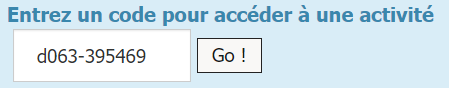
\includegraphics[scale=0.5]{td04_capcode}
	\end{center}
	\item laissez-vous guider sur le \cpy{notebook} et répondez aux différentes questions !
	\begin{center}
		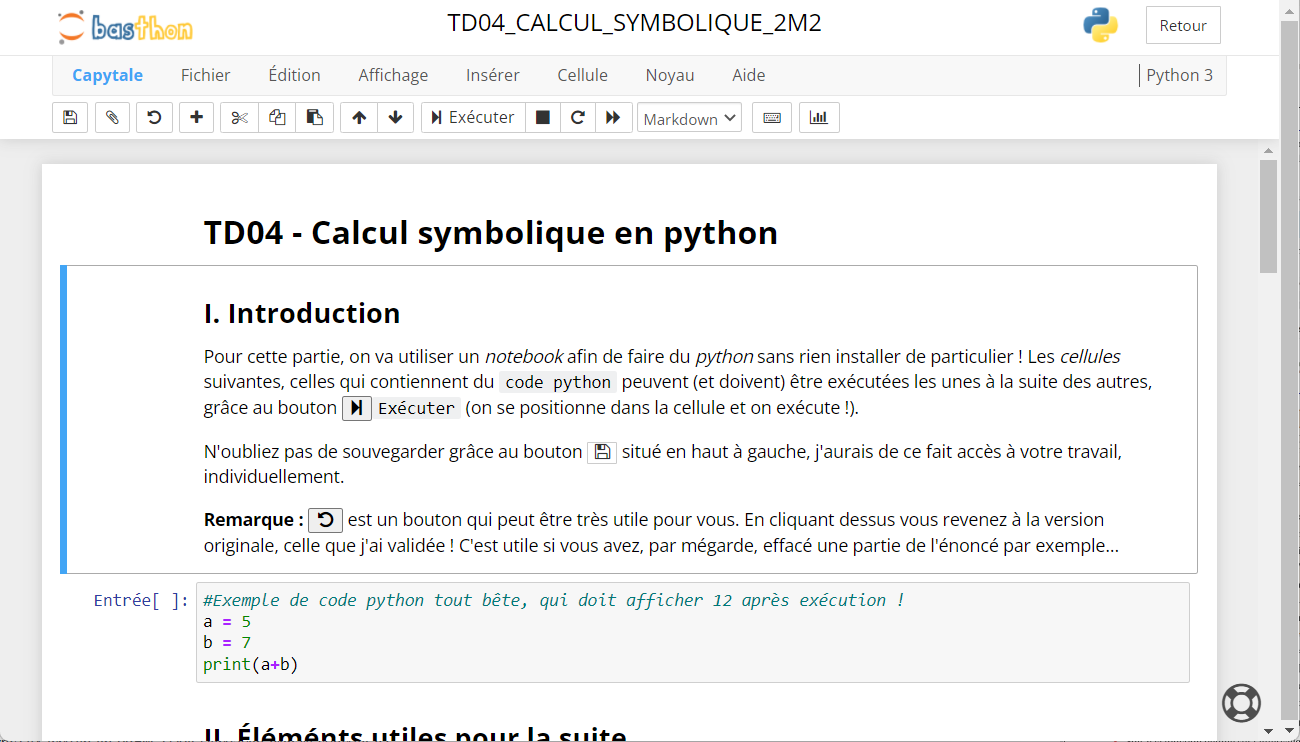
\includegraphics[scale=0.5]{td04_capcap}
	\end{center}
\end{itemize}

\medskip

\end{document}

\clearpage

% !TeX TXS-program:compile = txs:///arara
% arara: lualatex: {shell: no, synctex: yes, interaction: batchmode}
% arara: pythontex: {rerun: modified} if found('pytxcode', 'PYTHONTEX#py')
% arara: lualatex: {shell: no, synctex: yes, interaction: batchmode} if found('pytxcode', 'PYTHONTEX#py')
% arara: lualatex: {shell: no, synctex: yes, interaction: batchmode} if found('log', '(undefined references|Please rerun|Rerun to get)')

\documentclass[a4paper,11pt]{article}
\usepackage[revgoku]{cp-base} %avec options possibles parmi breakable (tcbox), sujetl (exos),  (pour faire "comme avant"), etc...
\graphicspath{{./graphics/}}
%variables
\donnees[classe=1\up{ère} 2M2,matiere={[SPÉ.MATHS]},typedoc=TD,numdoc=5,titre={Étude de salaires},mois=Mars,annee=2022]

%formatage
\author{Pierquet}
\title{\nomfichier}
\hypersetup{pdfauthor={Pierquet},pdftitle={\nomfichier},allbordercolors=white,pdfborder=0 0 0,pdfstartview=FitH}
%divers
\lhead{\entete{\matiere}}
\chead{\entete{\lycee}}
\rhead{\entete{\classe{} - \mois{} \annee}}
%\rhead{\entete{\classe{} - Chapitre }}
\lfoot{\pied{\matiere}}
\cfoot{\logolycee{}}
\rfoot{\pied{\numeropagetot}}

\begin{document}

\pagestyle{fancy}

\part{TD05 - Étude de salaires}

\smallskip

\nomprenomtcbox

\smallskip

Camille et Dominique ont été embauchés au même moment dans une entreprise et ont négocié leur contrat :

\begin{itemize}%[label=\scriptsize\faIcon{money-bill-alt}]
	\item[\scriptsize\faIcon{money-bill-alt}] Camille a commencé en 2018 avec un salaire annuel de \num{14400}\,€ ;
	\item[\scriptsize\faIcon{money-bill-alt}] le salaire de Dominique était, cette même année, de \num{13200}\,€ ;
	\item[\scriptsize\faChartLine] le salaire de Camille augmente de 600\,€ par an ;
	\item[\scriptsize\faChartLine] celui de Dominique augmente de 4\,\% par an. 
\end{itemize} 
%
\begin{enumerate}
	\item Quels étaient les salaires annuels de Camille et de Dominique en 2019 ? En 2020 ? Justifier les réponses.
	\item \textbf{Étude du salaire de Camille.} On note $c_n$ le salaire de Camille en l’année $2018+n$. On a donc $c_0 = \num{14400}$.
	\begin{enumerate}
		\item Quelle est la nature de la suite $\suiten[c]$ ? Justifier la réponse.
		\item Déterminer l'expression de $c_n$ en fonction de $n$. 
		\item Calculer le salaire de Camille en 2028.
		\item Déterminer, en détaillant la méthode, en quelle année le salaire de Camille dépassera \num{25000}\,€. 
	\end{enumerate}
	\item \textbf{Étude du salaire de Dominique.} On note $d_n$ le salaire de Dominique en l’année $2018+n$. 
	\begin{enumerate}
		\item Préciser la valeur de $d_0$.
		\item Exprimer $d_{n+1}$ en fonction de $d_n$ puis en déduire la nature de la suite $\suiten[d]$.
		\item Déterminer l'expression de $d_n$ en fonction de $n$.
		\item Calculer le salaire de Dominique en 2028. On arrondira le résultat à l’euro. 
	\end{enumerate}
	\item \textbf{Évolution des deux salaires.} On veut déterminer à partir de quelle année le salaire de Dominique dépassera celui de Camille. Pour cela, on dispose du programme incomplet ci-dessous écrit 
	en langage \calgpython.
	\begin{enumerate}
		\item Compléter les quatre parties en pointillé du programme ci-dessous : 
		\begin{envpython}[12cm]
			def algo() : 
				C = 14400
				D = 13200
				n = 0
				while .................. :
					C = ................
					D = ................
					n = ................
				return n
		\end{envpython}
		\item Déterminer, en détaillant, en quelle année le salaire de Dominique dépassera celui de Camille.
	\end{enumerate}
	\item \textbf{Salaires cumulés entre 2018 et 2028.}
	\begin{enumerate}
		\item Calculer la somme $\sum_{i=0}^{10} d_i = d_0+d_1+\ldots+d_{10}$ et interpréter le résultat.
		\item Déterminer, en détaillant, le montant total des salaires perçus par Camille entre 2018 et 2028.
		\item Compléter les algorithmes suivants, écrits en \calgpython, afin qu'ils permettent de retrouver le résultat des questions \ptno{5}\pta{a} et \ptno{5}\pta{b}.
	\end{enumerate}
	\begin{minipage}{0.45\textwidth}
		\begin{envpython}[8.5cm]
			def cumul_camille() : 
				C = 14400
				S = 14400 
				for i in range(10):
					C = ................
					S = S + ............
				return ...
		\end{envpython}
	\end{minipage}\hfill
	\begin{minipage}{0.45\textwidth}
		\begin{envpython}[8.5cm]
			def cumul_dominique() : 
				D = .....
				S = 13200 
				for i in range(10):
					D = ................
					S = S + ............
				return ...
		\end{envpython}
	\end{minipage}
\end{enumerate}

\end{document}

\clearpage

% !TeX TXS-program:compile = txs:///arara
% arara: lualatex: {shell: no, synctex: yes, interaction: batchmode}
% arara: pythontex: {rerun: modified} if found('pytxcode', 'PYTHONTEX#py')
% arara: lualatex: {shell: no, synctex: yes, interaction: batchmode} if found('pytxcode', 'PYTHONTEX#py')
% arara: lualatex: {shell: no, synctex: yes, interaction: batchmode} if found('log', '(undefined references|Please rerun|Rerun to get)')

\documentclass[a4paper,11pt]{article}
\usepackage[revgoku]{cp-base}
\graphicspath{{./graphics/}}
%variables
\donnees[%
	classe=1\up{ère} 2M2,
	matiere={[SPÉ.MATHS]},
	typedoc=TD,
	numdoc=06,
	titre={Optimisation au rugby},
	mois=Mai,
	annee=2022
	]

%formatage
\author{Pierquet}
\title{\nomfichier}
\hypersetup{pdfauthor={Pierquet},pdftitle={\nomfichier},allbordercolors=white,pdfborder=0 0 0,pdfstartview=FitH}
%divers
\lhead{\entete{\matiere}}
\chead{\entete{\lycee}}
\rhead{\entete{\classe{} - \mois{} \annee}}
%\rhead{\entete{\classe{} - Chapitre }}
\lfoot{\pied{\matiere}}
\cfoot{\logolycee{}}
\rfoot{\pied{\numeropagetot}}

\begin{document}

\pagestyle{fancy}

\part{TD06 - Optimisation au rugby}

\smallskip

\nomprenomtcbox

\medskip

Lors d'un match de rugby, un joueur doit transformer un essai qui a été marqué au point $E$ (voir figure ci-contre) situé à l'extérieur du segment $[AB]$.

La transformation consiste à taper le ballon par un coup de pied depuis un point $T$ que le joueur a le droit de choisir n'importe où sur le segment $[EM]$ perpendiculaire à la droite $(AB)$ sauf en $E$. La transformation est réussie si le ballon passe entre les poteaux repérés par les points $A$ et $B$ sur la figure.

\begin{center}
	\definecolor{field}{RGB}{0,156,0}
	\begin{tikzpicture}[x=0.08cm,y=0.08cm,line join=bevel,font=\sffamily\large]
		\filldraw[field!75] (-62.5,-37.5) rectangle (62.5,37.5) ;
		\draw[white,ultra thick] (-60,-35) rectangle (60,35) ;
		\draw[white,ultra thick] (0,-35)--(0,35) (-50,-35)--(-50,35) (50,-35)--(50,35) ;
		\filldraw[white] (-50,-2.8) circle[radius=3pt] node[left=5pt] {A} (50,-2.8) circle[radius=3pt] (-50,2.8) circle[radius=3pt] node[left=5pt] {B} (50,2.8) circle[radius=3pt] ;
		\draw[ultra thick,white,densely dashed] (-50,-27.8)--(0,-27.8) ;
		\draw[ultra thick,white,densely dashed] (-50,-2.8)--(-20,-27.8)--(-50,2.8) ;
		\draw (0,37.5) node[above] {Terrain vu de dessus} ;
		\draw[white] (-20,-27.8) node[below=3pt] {T} ; \draw[white] (0,-27.8) node[right=2pt] {M} ; \draw[white] (-50,-27.8) node[left=2pt] {E} ;
		\draw[white] (-35,-27.8) node[below=1pt] {$\mathsf{x}$} ;
		\draw[white] (0,0) node[right=1pt] {\rotatebox{90}{Ligne médiane}} ;
		\draw[white] (50,0) node[right=1pt] {\rotatebox{90}{Limite du terrain}} ;
		\draw (-20,-27.8) node {\scriptsize\faFootballBall} ;
		\draw (-50,-27.8) node {\scriptsize\faFootballBall} ;
	\end{tikzpicture}
\end{center}

Pour maximiser ses chances de réussite, le joueur tente de déterminer la position du point $T$ qui rend l'angle $\widehat{ATB}$ le plus grand possible.

\medskip

Le but de cet exercice est donc de rechercher s'il existe une position du point $T$ sur le segment $[EM]$ pour laquelle l'angle $\widehat{ATB}$ est maximum et, si c'est le cas, de déterminer une valeur approchée de cet angle.

Dans toute la suite, on note $x$ la longueur $ET$, qu'on cherche à déterminer.

\smallskip

On donne les dimensions : $EM=50$~m, $EA=25$~m et $AB=5,6$~m ; et on note $\alpha$ une mesure de l'angle $\widehat{ATB}$.

\smallskip

On se place dans le repère $\left( E\,;\vect{i},\vect{j} \right)$ de sorte que, dans ce repère, on a $T\coordpl{x}{0}$, $M\coordpl{50}{0}$ et $A\coordpl{0}{25}$. 

\begin{enumerate}
	\item Préciser l'intervalle, noté $I$, dans lequel peut varier $x$.
	\item Déterminer les coordonnées du point $B$.
	\item Dans cette question, on suppose que $x=15$.
	\begin{enumerate}
		\item Déterminer les coordonnées des vecteurs $\vect{TA}$ et $\vect{TB}$.
		\item Déterminer la valeur de $\vect{TA} \cdot \vect{TB}$.
		\item Calculer les longueurs $TA$ et $TB$.
		\item En utilisant une autre expression du produit scalaire $\vect{TA} \cdot \vect{TB}$, déterminer une valeur approchée, au centième de degré près, de l'angle $\widehat{ATB}$.
	\end{enumerate}
	\item Dans cette question, on ne connaît pas la valeur de $x$.
	\begin{enumerate}
		\item Déterminer, en fonction de $x$, les coordonnées des vecteurs $\vect{TA}$ et $\vect{TB}$.
		\item Déterminer, en fonction de $x$, la valeur de $\vect{TA} \cdot \vect{TB}$.
		\item Calculer, en fonction de $x$, les longueurs $TA$ et $TB$.
		\item En utilisant une autre expression du produit scalaire $\vect{TA} \cdot \vect{TB}$, vérifier que : \[\cos\left(\widehat{ATB}\right)=\dfrac{x^2+765}{\sqrt{x^2+625} \times \sqrt{x^2+936,36}}.\]
	\end{enumerate}
	\item On considère donc la fonction $f$ définie sur $I$ (donné dans la question \ptno{1}) par \[ f(x)=\cos^{-1} \left( \dfrac{x^2+765}{\sqrt{x^2+625} \times \sqrt{x^2+936,36}} \right).\]
	\begin{enumerate}
		\item En utilisant la calculatrice, paramétrée en degré, compléter le tableau de valeurs (arrondies à $0,01$) :
		
		\begin{center}
			\renewcommand\arraystretch{1.1}
			\begin{tabularx}{\linewidth}{|*{10}{Y|}}
				\hline
				$x$ & $5$ & $10$ & $15$ & $20$ & $21$ & $22$&$23$&$24$&$25$ \\ \hline
				$f(x)$ &&&$4,85$&&&&&& \\ \hline
				\hline
				$x$ & $26$ & $27$ & $28$ & $29$ & $30$ & $35$ & $40$ & $45$ & $50$ \\ \hline
				$f(x)$ &&&&&&&&&$4,90$ \\ \hline
			\end{tabularx}
		\end{center}
		\item Dans le repère suivant, tracer la courbe $\mathscr{C}_f$ représentative de la fonction $f$ :
		
		\begin{center}
			\tunits{0.3}{1.5}
			\tdefgrille{0}{50}{2.5}{0.5}{0}{6}{0.5}{0.1}
			\begin{tikzpicture}[x=\xunit cm,y=\yunit cm]
				\def\f{acos((x*x+765)/(sqrt(x*x+625)*sqrt(x*x+936.36)))}
				\tgrilles[line width=0.3pt,lightgray!75] ;
				\tgrillep[line width=0.6pt,lightgray] ;
				\axestikz* ; \axextikz{0,5,...,45} ; \axeytikz{0,0.5,...,5.5} ;
				%\draw[very thick,red,domain=0:50,samples=500] plot function{\f*180/pi} ;
				\foreach \Point in {(0,0),(15,4.85),(50,4.90)} \filldraw[red] \Point circle[radius=2.5pt] ;
			\end{tikzpicture}
		\end{center}
		\vspace{-0.25cm}
		\item Estimer graphiquement le maximum de $f$ ainsi que la valeur de $x$ pour laquelle $f$ est maximale.
		\item Conclure quant au problème initial.
	\end{enumerate}
	\item On admet, après étude mathématique \og plus poussée \fg{} que, lorsque l'essai est marqué à l'extérieur des poteaux et à une distance $m$ du poteau ($m$ correspond à la longueur $EA$ et est typiquement entre 2 et 32 mètres), la valeur de $x$ qui rend maximal l'angle $\widehat{ATB}$ est donnée par \[ x = \sqrt{ m^2 + 5,6m}.\]
	\begin{enumerate}
		\item Vérifier que pour $m=25$, on retrouve approximativement la valeur de $x$ déterminée à la question \ptno{5}\pta{c}.
		\item Si l'essai est marqué à peu près au milieu de la distance entre le poteau et le coin de l'aire de jeu (la largeur d'un terrain de rugby est d'environ 70~m), déterminer la position la plus favorable pour le transformer.
		\item Compléter l'algorithme \calgpython{} suivant de sorte qu'un appel à la \calg{fonction} \cpy{distance} renvoie la distance optimale pour la transformation lorsque que l'essai est marqué à \cpy{m} mètres de l'un des poteaux :
		\begin{envpython}[14cm]
			from math import sqrt     #on importe la fonction racine
			def distance(m):
				res = ..............................................
				return res
		\end{envpython}
		\item Vérifier, sur quelques exemples, que $x \approx m+2,5$ semble être une bonne approximation de la distance optimale.
	\end{enumerate}
\end{enumerate}



\end{document}

\clearpage

% !TeX TXS-program:compile = txs:///arara
% arara: lualatex: {shell: no, synctex: yes, interaction: batchmode}
% arara: pythontex: {rerun: modified} if found('pytxcode', 'PYTHONTEX#py')
% arara: lualatex: {shell: no, synctex: yes, interaction: batchmode} if found('pytxcode', 'PYTHONTEX#py')
% arara: lualatex: {shell: no, synctex: yes, interaction: batchmode} if found('log', '(undefined references|Please rerun|Rerun to get)')

\documentclass[a4paper,11pt]{article}
\usepackage[revgoku]{cp-base}
\graphicspath{{./graphics/}}
%variables
\donnees[%
	classe=1\up{ère} 2M2,
	matiere={[SPÉ.MATHS]},
	typedoc=TD,
	numdoc=07,
	mois=Mai,
	annee=2022
	]

%formatage
\author{Pierquet}
\title{\nomfichier}
\hypersetup{pdfauthor={Pierquet},pdftitle={\nomfichier},allbordercolors=white,pdfborder=0 0 0,pdfstartview=FitH}
%divers
\lhead{\entete{\matiere}}
\chead{\entete{\lycee}}
\rhead{\entete{\classe{} - \mois{} \annee}}
%\rhead{\entete{\classe{} - Chapitre }}
\lfoot{\pied{\matiere}}
\cfoot{\logolycee{}}
\rfoot{\pied{\numeropagetot}}

\begin{document}

\pagestyle{fancy}

\part{TD07 - Probabilités et variable aléatoire}

\smallskip

%\nomprenomtcbox
%
%\medskip

On dispose d'un paquet de cartes contenant un nombre identique de cartes de la catégorie \og Sciences \fg{} et de la catégorie \og Économie \fg. Une question liée à un de ces deux thèmes figure sur chaque carte.

Les cartes sont mélangées et on en tire une au hasard dans le paquet. Ensuite, on essaye de répondre à la question posée.

\smallskip

Un groupe de copains participe à ce jeu. Connaissant leurs points forts et leurs faiblesses, on estime qu'il a :

\begin{itemize}
	\item 3 chances sur 4 de donner la bonne réponse lorsqu'il est interrogé en sciences ;
	\item 1 chance sur 8 de donner la bonne réponse lorsqu'il est interrogé en économie.
\end{itemize}

On note $S$ l'évènement \og La question est dans la catégorie Sciences \fg{} et $B$ l'évènement \og La réponse donnée par le groupe est bonne \fg.

\bigskip

\textbf{-- Partie A --}
%
\begin{enumerate}
	\item Construire un arbre pondéré modélisant la situation présentée dans l'énoncé.
	\item Calculer $P(B \cap S)$.
	\item Déterminer la probabilité que le groupe de copains réponde correctement à la question posée.
	\item Calculer $P_B(E)$ et interpréter le résultat dans le contexte de l'exercice.
	\item Les évènements $S$ et $B$ sont-ils indépendants ? Justifier.
	\item On choisit successivement, et avec remise, deux cartes du paquet. Déterminer la probabilité que la bonne réponse est donnée pour les deux cartes.
\end{enumerate}

\textbf{-- Partie B --}

\medskip

Pour participer à ce jeu, on doit payer 5\,€ de droit d'inscription. On recevra :

\begin{itemize}
	\item 10\,€ si on est interrogé en sciences et que la réponse est correcte ;
	\item 30\,€ si on est interrogé en économie et que la réponse est correcte ;
	\item rien si la réponse donnée est fausse.
\end{itemize}

Soit $X$ la variable aléatoire qui, à chaque partie jouée, associe son gain. On appelle gain la différence en euros entre ce qui est reçu et les 5\,€ de droit d'inscription.

\begin{enumerate}
	\item Déterminer (sous forme de tableau) la loi de probabilité de $X$.
	\item On considère la fonction \cpy{jeu} ci-dessous en langage \calgpython, pour laquelle les paramètres \cpy{L} et \cpy{G} sont des listes.
		
	\begin{envpython}[13cm]
		def jeu(L,G) :
			n = len(L)
			E = 0
			for i in range(n) :
				E = E + L[i]*G[i]
			return E
	\end{envpython}
	\begin{enumerate}
		\item Que retourne la fonction \cpy{jeu} avec comme paramètres les listes ci-dessous ?
		\begin{itemize}
			\item \cpy{L = [-5 , 5 , 25]} ;
			\item \cpy{G = [0.5625 , 0.375 , 0.0625]}
		\end{itemize}
		\item Interpréter le résultat dans le contexte de l'exercice.
	\end{enumerate}
\end{enumerate}






\end{document}

\clearpage

% !TeX TXS-program:compile = txs:///arara
% arara: lualatex: {shell: no, synctex: yes, interaction: batchmode}
% arara: pythontex: {rerun: modified} if found('pytxcode', 'PYTHONTEX#py')
% arara: lualatex: {shell: no, synctex: yes, interaction: batchmode} if found('pytxcode', 'PYTHONTEX#py')
% arara: lualatex: {shell: no, synctex: yes, interaction: batchmode} if found('log', '(undefined references|Please rerun|Rerun to get)')

\documentclass[a4paper,11pt]{article}
\usepackage[revgoku]{cp-base}
\graphicspath{{./graphics/}}
%variables
\donnees[%
	classe=1\up*{ère} 2M2,
	matiere={[SPÉ.MATHS]},
	typedoc=TD,
	numdoc=08,
	mois=Juin,
	annee=2022
	]

%formatage
\author{Pierquet}
\title{\nomfichier}
\hypersetup{pdfauthor={Pierquet},pdftitle={\nomfichier},allbordercolors=white,pdfborder=0 0 0,pdfstartview=FitH}
%divers
\lhead{\entete{\matiere}}
\chead{\entete{\lycee}}
\rhead{\entete{\classe{} - \mois{} \annee}}
\lfoot{\pied{\matiere}}
\cfoot{\logolycee{}}
\rfoot{\pied{\numeropagetot}}

\begin{document}

\pagestyle{fancy}

\part{TD08 - Fonction exponentielle en situation}

Une start-up fabrique entre 100 et 2\,000 ordinateurs par jour. On admet que si la start-up fabrique $x$ \textbf{centaines d'ordinateurs}, le bénéfice en \textbf{centaines d'euros} est modélisé par : \[ f(x)=80x\,\e^{-0,2x} \text{, avec } x \in \intervFF{1}{20}.\]
%
On note $f'$ la dérivée de la fonction $f$, et on note $\mathscr{C}_f$ sa courbe représentative dans un repère orthogonal, donnée en ci-dessous.

\begin{center}
	\begin{tikzpicture}[x=0.6cm,y=0.06cm,xmin=0,xmax=21,xgrille=1,xgrilles=0.2,ymin=0,ymax=155,ygrille=10,ygrilles=2]
		\tgrilles \tgrillep \axestikz*
		\axextikz[size=\small]{0,1,...,20} \axeytikz[size=\small]{0,10,...,150}
		%\clip (\xmin,\ymin) rectangle (\xmax,\ymax) ;
		\draw[very thick,red,domain=1:20,samples=100] plot (\x,{80*\x*exp(-0.2*\x)}) ;
		\draw[red] (1.5,65) node {\large $\mathscr{C}_f$} ;
	\end{tikzpicture}
\end{center}

\textbf{\large Partie A -- Étude graphique}

\medskip

À l'aide du graphique et en laissant les traits de construction apparents :

\begin{enumerate}
	\item déterminer le maximum de la fonction $f$ sur l'intervalle $\intervFF{1}{20}$ ;
	\item résoudre l'équation $f(x)=100$, avec la précision permise par le graphique.
\end{enumerate}

\textbf{\large Partie B - Étude de la fonction $\grasmaths{f}$}

\begin{enumerate}
	\item 
	\begin{enumerate}
		\item Justifier que, pour tout $x$ appartenant $\intervFF{1}{20}$, on a $f'(x)=\e^{-0,2x}(80-16x)$.
		\item Étudier le signe de $f'(x)$ sur l'intervalle $\intervFF{1}{20}$.
		\item En déduire le tableau de variation de la fonction $f$ (les images seront, si besoin, arrondies au centième).
	\end{enumerate}
	\item Démontrer que l'équation $f(x) = 100$ admet une unique solution sur l'intervalle $\intervFF{1}{5}$ puis en déterminer, à l'aide de la calculatrice, une valeur approchée au centième.
	
	\smallskip
	
	On admet que sur l'intervalle $\intervFF{5}{20}$ l'équation $f(x)=100$ admet également une unique solution égale à environ $10,76$.
\end{enumerate}

\textbf{\large Partie C -- Interprétation}

\begin{enumerate}
	\item Déterminer le bénéfice maximal à l'euro près réalisé par la start-up et le nombre d'ordinateurs fabriqués pour le réaliser
	\item Entre quelles valeurs doit être compris le nombre d'ordinateurs fabriqués pour que la start-up réalise un bénéfice supérieur ou égal à 10\,000 euros ?
\end{enumerate}

\end{document}

\clearpage

% !TeX TXS-program:compile = txs:///arara
% arara: lualatex: {shell: no, synctex: yes, interaction: batchmode}
% arara: pythontex: {rerun: modified} if found('pytxcode', 'PYTHONTEX#py')
% arara: lualatex: {shell: no, synctex: yes, interaction: batchmode} if found('pytxcode', 'PYTHONTEX#py')
% arara: lualatex: {shell: no, synctex: yes, interaction: batchmode} if found('log', '(undefined references|Please rerun|Rerun to get)')

\documentclass[a4paper,11pt]{article}
\usepackage[revgoku]{cp-base}
\graphicspath{{./graphics/}}
%variables
\donnees[%
	classe=1\up*{ère} 2M2,
	matiere={[SPÉ.MATHS]},
	typedoc=TD,
	numdoc=08,
	mois=Juin,
	annee=2022
	]

%formatage
\author{Pierquet}
\title{\nomfichier}
\hypersetup{pdfauthor={Pierquet},pdftitle={\nomfichier},allbordercolors=white,pdfborder=0 0 0,pdfstartview=FitH}
%divers
\lhead{\entete{\matiere}}
\chead{\entete{\lycee}}
\rhead{\entete{\classe{} - \mois{} \annee}}
\lfoot{\pied{\matiere}}
\cfoot{\logolycee{}}
\rfoot{\pied{\numeropagetot}}

\begin{document}

\pagestyle{fancy}

\part{TD08 - Fonction exponentielle en situation (Correction)}

\smallskip

\textbf{\large Partie A}
%
\begin{enumerate}
	\item Graphiquement, le \textcolor{purple}{maximum} de la fonction $f$ est estimé à 147 (pour $x=5$).
	\item Graphiquement, les \textcolor{ForestGreen}{solutions} de $f(x)=100$ sont approximativement $1,8$ et $10,8$.
\end{enumerate}

\begin{center}
	\begin{tikzpicture}[x=0.8cm,y=0.08cm,xmin=0,xmax=21,xgrille=1,xgrilles=0.2,ymin=0,ymax=155,ygrille=10,ygrilles=2]
		\tgrilles \tgrillep \axestikz*
		\axextikz[size=\small]{0,1,...,20} \axeytikz[size=\small]{0,10,...,150}
		%\clip (\xmin,\ymin) rectangle (\xmax,\ymax) ;
		\draw[very thick,red,domain=1:20,samples=500] plot (\x,{80*\x*exp(-0.2*\x)}) ;
		\draw[red] (1.5,65) node {\Large $\mathscr{C}_f$} ;
		\draw[very thick,densely dashed,purple] (5,0) |- (0,147.15) ;
		\filldraw[purple] (5,147.15) circle[radius=2.5pt] ;
		\draw[very thick,densely dashed,ForestGreen] (1.79,0) |- (0,100) (10.76,0) |- (0,100) ;
		\filldraw[ForestGreen] (1.79,100) circle[radius=2.5pt] (10.76,100) circle[radius=2.5pt] ;
	\end{tikzpicture}
\end{center}

\textbf{\large Partie B}
%
\begin{enumerate}
	\item
	\begin{enumerate}
		\item La fonction $f$ est dérivable sur $\intervFF{1}{20}$ par produit, avec $\begin{dcases} u=80x \\ v=\e^{-0,2x} \end{dcases}$ et $\begin{dcases} u'=80 \\ v=-0,2\e^{-0,2x} \end{dcases}$.
		
		Ainsi $f'(x)=u'v+v'u=80 \times \e^{-0,2x} + \left(-0,2\e^{-0,2x}\right) \times 80x = 80 \e^{-0,2x} \times (1-0,2x)$.
		\item $f'(x)$ se présente comme un produit, avec déjà $80\e^{-0,2x} > 0$, et $1-0,2x=0 \ssi 0,2x=1 \ssi x=5$.
		
		\begin{center}
			\begin{tikzpicture}
				\tkzTabInit{$x$/1,$80\e^{-0,2x}$/1,$(1-{0,2}x)$/1,$f'(x)$/1}{$1$,$5$,$20$}
				\tkzTabLine{,+,t,+,}
				\tkzTabLine{,+,z,-,}
				\tkzTabLine{,+,z,-,}
				\aidesignetkztabPL[code=da-,racines={5},couleur=orange]{2}
			\end{tikzpicture}
		\end{center}
		\pagebreak
		\item On en déduit le tableau de variations de la fonction $f$ (les images étant arrondies au centième) :
		
		\begin{center}
			\begin{tikzpicture}
				\tkzTabInit[deltacl=0.8]{$x$/1,$f'(x)$/1,$f$/2}{$1$,$5$,$20$}
				\tkzTabLine{,+,z,-,}
				\tkzTabVar{-/${65,50}$,+/${147,15}$,-/${29,31}$}
				\tkzTabVal[draw]{1}{2}{0.55}{\small \red $\alpha$}{\small \red 100}
				\tkzTabVal[draw]{2}{3}{0.55}{\small \red $\beta$}{\small \red 100}
			\end{tikzpicture}
		\end{center}
	\end{enumerate}
	\item D'après le tableau de variations, $f$ est croissante sur $\intervFF{1}{5}$ et $\begin{dcases} f(1) < 100 \\ f(5) > 100 \end{dcases}$.
	
	L'équation $f(x)=100$ admet de ce fait une unique solution ($\alpha$) sur $\intervFF{1}{5}$.
	
	D'après la fonction TABLE de la calculatrice, $\left. \begin{dcases} f(1,78) \approx 99,474 \\ f(1,79) \approx 100,11 \end{dcases} \right| \Rightarrow \alpha \approx 1,79$.
\end{enumerate}

\begin{pointcalc}
	\hfill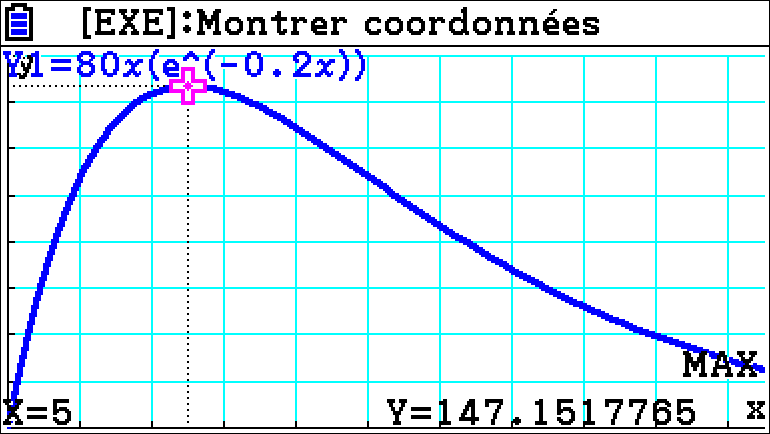
\includegraphics[height=3cm]{td08_corr_a}~~~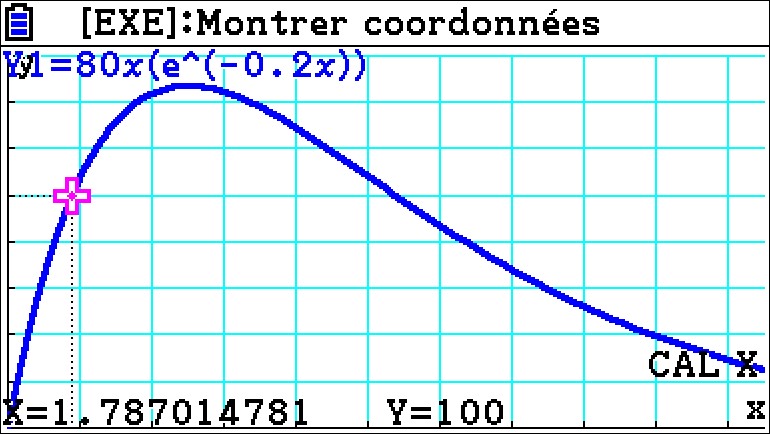
\includegraphics[height=3cm]{td08_corr_b}~~~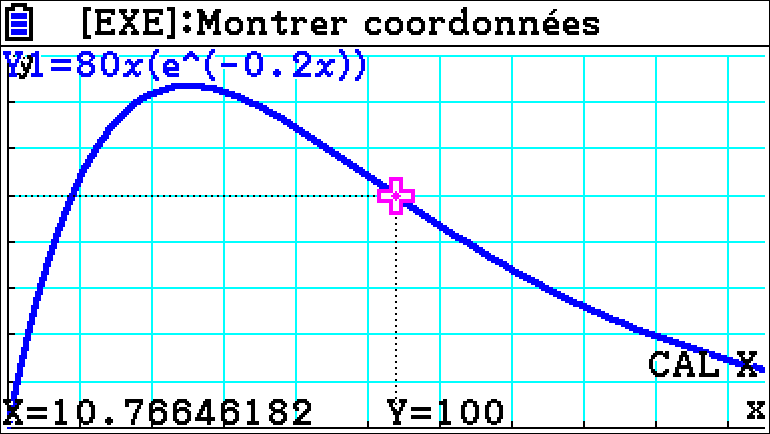
\includegraphics[height=3cm]{td08_corr_c}\hfill~
\end{pointcalc}

\textbf{\large Partie C}
%
\begin{enumerate}
	\item D'après la question \textbf{A.}\ptno{1} ou la question \textbf{B.}\ptno{1}\pta{c}, on peut affirmer que la bénéfice maximal réalisé par la start-up est de \num{14715}\,€ ($147,15$ centaines) pour 500 (5 centaines) d'ordinateurs fabriqués.
	\item D'après la question \textbf{A.}\ptno{2} ou la question \textbf{B.}\ptno{2}, pour que la start-up réalise un bénéfice supérieur ou égal à 10\,000\,€, elle doit fabriquer entre 179 et 1\,076 ($\alpha$ et $\beta$ centaines) ordinateurs.
\end{enumerate}

\end{document}

\clearpage

\makeatletter
\renewcommand\exonum[2][]{
	\def\hrulefill{\leavevmode\leaders\hrule height 1.1pt\hfill\kern\z@}%épaisseur
	\ifthenelse{\equal{#2}{1}}%
	{%
		\def\pts{point}
	}%
	{%
		\def\pts{points}
	}
	\addtocounter{numexos}{1}{\sffamily\textbf{\LARGE \textcolor{titrebleu}{Exercice \thenumexos#1~{\color{titrebleu}\hrulefill~(#2 \pts)}}}}%
	\def\hrulefill{\leavevmode\leaders\hrule height 0.4pt\hfill\kern\z@}
}
\newcommand\exoannexe[1]{
	\def\hrulefill{\leavevmode\leaders\hrule height 1.1pt\hfill\kern\z@}%épaisseur
	{\sffamily\textbf{\LARGE \textcolor{titrebleu}{Annexe Exercice#1~{\color{titrebleu}\hrulefill}}}}%
	\def\hrulefill{\leavevmode\leaders\hrule height 0.4pt\hfill\kern\z@}
}
\newcommand\exocours[1]{
	\def\hrulefill{\leavevmode\leaders\hrule height 1.1pt\hfill\kern\z@}%épaisseur
	{\sffamily\textbf{\LARGE \textcolor{titrebleu}{Questions de cours~{\color{titrebleu}\hrulefill~(#1 points)}}}}%
	\def\hrulefill{\leavevmode\leaders\hrule height 0.4pt\hfill\kern\z@}
}
\newcommand\exogenerique[2]{
	\def\hrulefill{\leavevmode\leaders\hrule height 1.1pt\hfill\kern\z@}%épaisseur
	{\sffamily\textbf{\LARGE \textcolor{titrebleu}{#1~{\color{titrebleu}\hrulefill~(#2)}}}}%
	\def\hrulefill{\leavevmode\leaders\hrule height 0.4pt\hfill\kern\z@}
}
\makeatother

\clearpage

% !TeX TXS-program:compile = txs:///arara
% arara: lualatex: {shell: no, synctex: yes, interaction: batchmode}
% arara: pythontex: {rerun: always}
% arara: lualatex: {shell: no, synctex: yes, interaction: batchmode}
% arara: lualatex: {shell: no, synctex: yes, interaction: batchmode} if found('log', 'undefined references')

\documentclass[a4paper,11pt]{article}
\usepackage[pythontex,sujet]{cp-base} %avec options possibles parmi breakable (tcbox), sujetl (exos),  (pour faire "comme avant"), etc...
\graphicspath{{./graphics/}}
%variables
\donnees[
	classe={1\up{ère} 2M2},matiere={[SPÉ.MATHS]},mois={Jeudi 30 Septembre},annee=2021,duree=1 heure,typedoc=DS,numdoc=1
	]
%formatage
\author{Pierquet}
\title{\nomfichier}
\hypersetup{pdfauthor={Pierquet},pdftitle={\nomfichier},allbordercolors=white,pdfborder=0 0 0,pdfstartview=FitH}
%divers
\lhead{\entete{\matiere}}
\chead{\entete{\lycee}}
\rhead{\entete{\classe{} - \mois{} \annee}}
\lfoot{\pied{\matiere}}
\cfoot{\logolycee{}}
\rfoot{\pied{\numeropagetot}}
\fancypagestyle{enteteds}{\fancyhead[L]{\entete{Durée : \duree}}}

\begin{document}

\pagestyle{fancy}

\thispagestyle{enteteds}

\setcounter{numexos}{0}

\part{DS01 - Second degré}

\smallskip

\begin{marker}$\leftrightsquigarrow$ Le sujet est à rendre avec la copie. $\leftrightsquigarrow$\end{marker}

\nomprenomtcbox

\medskip

\exonum{6}

\medskip

Soit $f(x)=ax^2+bx+c$ un polynôme du second degré (avec $a \neq 0$), dont la courbe représentative dans un repère orthogonal est une parabole $\mathcallig{P}$.
%
\begin{enumerate}
	\item 
	\begin{enumerate}
		\item Rappeler les formules permettant de calculer $\alpha$ et $\beta$.
		\item Écrire l'expression de $f(x)$ dans laquelle apparaissent $\alpha$ et $\beta$. Comment s'appelle cette forme ?
	\end{enumerate}
	\item 
	\begin{enumerate}
		\item Comment s'appelle le nombre $\Delta$ ? Rappeler sa formule de calcul.
		\item Rappeler les formules de calcul des deux racines $x_1$ et $x_2$ lorsqu'elles existent.
		\item Écrire l'expression de $f(x)$ dans laquelle apparaissent $x_1$ et $x_2$. Comment s'appelle cette forme ?
	\end{enumerate}
	\item Si la parabole $\mathcallig{P}$ représentant le trinôme est \og ouverte vers le haut \fg{} et ne coupe pas l'axe des abscisses, que peut-on en déduire ?
\end{enumerate}

\medskip

\exonum{4}

\medskip

Écrire chacun des polynômes ci-dessous dans la forme demandée :
%
\begin{enumerate}
	\item $P(x)=-2(x+1)(x-5)$ sous forme développée réduite.
	\item $Q(x)=3x^2+6x-7$ sous forme canonique.
	\item $R(x)=x^2-6x+5$ sous forme factorisée.
\end{enumerate}

\medskip

\exonum{5}
%
\begin{enumerate}
	%\item Déterminer, en justifiant, le tableau de variations de la fonction $f$ définie par $f(x)=-2x^2+4x+7$.
	\item Résoudre l'équation $0,5x^2-x-12=0$.
	\item Résoudre l'équation $(x-5)(x^2+x+1)=0$.
	\item Résoudre l'équation $\dfrac{7x}{x+2}={x-5}$ (pour $x \neq -2$).
\end{enumerate}

\medskip

\exonum{5}

\medskip

Soit $f$ et $g$ deux polynômes du second degré définis par $f(x)=3x^2 + 12x + 27$ et $g(x)=-2x^2-7x+15$.
%
\begin{enumerate}
	\item 
	\begin{enumerate}
		\item Déterminer la forme canonique de $f$.
		\item En déduire le tableau de variation de la fonction $f$.
	\end{enumerate}
	\item 
	\begin{enumerate}
		\item Déterminer les racines de la fonction $g$.
		\item Résoudre l'équation $f(x)=g(x)$.
	\end{enumerate}
\end{enumerate}

\medskip

\exonum[ (BONUS)]{1}

\medskip

On considère l'algorithme suivant, donné en langage \calgpython{} :
%
\begin{envpython}[8cm]
def mystere(a,b,c) :
	res = b**2-4*a*c
	return res
\end{envpython}
%
Que renverra la commande \cpy{mystere(1,1,1)} ?


%\medskip
%
%\exonum{5}
%
%\smallskip
%
%On donne ci-dessous la courbe représentative d'un polynôme du second degré $f(x)$.
%
%\begin{center}
%	\tunits{0.6}{0.6}
%	\tdefgrille{-1}{7}{1}{0.5}{-3}{7}{1}{0.5}
%	\begin{tikzpicture}[x=\xunit cm,y=\yunit cm]
%		\tgrillep[densely dashed,line width=0.6pt,gray!50]
%		\draw[->,line width=1.25pt] (\xmin,0) -- (\xmax,0);
%		\draw[->,line width=1.25pt] (0,\ymin) -- (0,\ymax);
%		\foreach \x in {-1,0,...,6} %à compléter avec itération ou complètement
%		\draw[line width=1.25pt] (\x,4pt) -- (\x,-4pt) node[below] {\footnotesize \num{\x}}; %éventuellement \xx et taille...
%		\foreach \y in {-3,-2,...,6}
%		\draw[line width=1.25pt] (4pt,\y) -- (-4pt,\y) node[left] {\footnotesize \num{\y}};
%		\draw[line width=1.25pt,red,domain=-1:7,samples=200] plot(\x,{0.5*(\x-3)*(\x-3)-2});
%	\end{tikzpicture}
%\end{center}
%
%\begin{enumerate}
%	\item \textit{Aucun calcul n'est attendu dans cette première question.}
%	\begin{enumerate}
%		\item Donner les valeurs de $\alpha$, $\beta$ et des racines si elles existent (inutile de justifier).
%		\item Sans faire de calcul, peut-on dire du coefficient $a$ ? Justifier.
%		\item Sans faire de calcul, que peut-on dire de $\Delta$ ? Justifier.
%	\end{enumerate}
%	\item Déterminer une expression (au choix) de la fonction $f(x)$.
%	\item \textbf{[Question bonus]} Dans un autre repère, représenter la courbe d'une fonction du second degré $g$ dans laquelle le coefficient $a$ (de plus haut degré) est négatif, et le $\Delta$ est nul.
%\end{enumerate}

\end{document}

\clearpage

% !TeX TXS-program:compile = txs:///lualatex

\documentclass[a4paper,11pt]{article}
\usepackage[sujet]{cp-base} %avec options possibles parmi breakable (tcbox), sujetl (exos),  (pour faire "comme avant"), etc...
\graphicspath{{./graphics/}}
%variables
\donnees[
	classe={1\up{ère} 2M2},matiere={[SPÉ.MATHS]},mois={Jeudi 21 Octobre},annee=2021,duree=1 heure,typedoc=DS,numdoc=2
]
%formatage
\author{Pierquet}
\title{\nomfichier}
\hypersetup{pdfauthor={Pierquet},pdftitle={\nomfichier},allbordercolors=white,pdfborder=0 0 0,pdfstartview=FitH}
%divers
\lhead{\entete{\matiere}}
\chead{\entete{\lycee}}
\rhead{\entete{\classe{} - \mois{} \annee}}
\lfoot{\pied{\matiere}}
\cfoot{\logolycee{}}
\rfoot{\pied{\numeropagetot}}
\fancypagestyle{enteteds}{\fancyhead[L]{\entete{Durée : \duree}}}

\begin{document}

\pagestyle{fancy}

\thispagestyle{enteteds}

\setcounter{numexos}{0}

\part{DS02 - Second degré, suites}

\smallskip

\nomprenomtcbox

\medskip

\exonum{5}

\begin{enumerate}
	\item Déterminer la forme canonique de la fonction $f(x)=-2x^2+8x-7$ puis en déduire son tableau de variations.
	\item Déterminer les éventuelles racines du trinômes $8x^2-10x+2$ puis son éventuelle factorisation.
	\item Résoudre les équations suivantes :
	\begin{enumerate}
		\item $-2x^2-2x-2=0$ ;
		\item $(x-3)(-x^2-3x+10)=0$ ;
		\item $x^2+6x+7=-2$.
	\end{enumerate}
\end{enumerate}

\bigskip

\exonum{6}

\begin{enumerate}
	\item On considère la suite $\suiten$ définie par $u_n = \dfrac{4}{n}+2$ pour tout entier naturel $n$ non nul.
	\begin{enumerate}
		\item Calculer les valeurs de $u_1$, $u_2$ et $u_3$.
		\item Déterminer une expression de la fonction $f$ telle que $u_n=f(n)$.
		\item Déterminer le 10\ieme{} terme de la suite $\suiten$.
	\end{enumerate}
	\item On considère la suite $\suiten[v]$ définie par $\begin{dcases} v_0 = 4 \\ v_{n+1}=\dfrac{v_n} {2+v_n} \end{dcases}$ pour tout entier naturel $n$.
	\begin{enumerate}
		\item Calculer les valeurs de $v_1$ et $v_2$.
		\item Déterminer une expression de la fonction $g$ telle que $v_{n+1}=g(v_n)$.
		\item En utilisant la calculatrice, déterminer la valeur de $v_{10}$.
	\end{enumerate}
	\item On considère la suite $\suiten[w]$ définie par $\begin{dcases} w_0 = 10 \\ w_{n+1}=n^2 + 2 + w_n \end{dcases}$ pour tout entier naturel $n$.
	\begin{enumerate}
		\item Calculer les valeurs de $w_1$ et $w_2$.
		\item En utilisant la calculatrice, déterminer la valeur de $w_{15}$.
	\end{enumerate}
\end{enumerate}

\bigskip

\exonum{3}

\begin{enumerate}
	\item 
	\begin{enumerate}
		\item À l'aide de la calculatrice, représenter (sur le graphique suivant) les 10 premiers termes de la suite $\suiten$ définie par $u_n=1+\dfrac{2}{n}$ pour tout entier $n$ non nul.
		\begin{center}
			\tunits{1}{1}
			\tdefgrille{0}{11}{1}{0.25}{0}{4}{1}{0.25}
			\begin{tikzpicture}[x=\xunit cm,y=\yunit cm]
				\tgrilles ;
				\tgrillep ;
				\draw[->,line width=1.25pt] (\xmin,0) -- (\xmax,0);
				\draw[->,line width=1.25pt] (0,\ymin) -- (0,\ymax);
				\foreach \x in {0,1,...,10}
				\draw[line width=1.25pt] (\x,4pt) -- (\x,-4pt) node[below] {\num{\x}};
				\foreach \y in {0,1,2,3}
				\draw[line width=1.25pt] (4pt,\y) -- (-4pt,\y) node[left] {\num{\y}};
			\end{tikzpicture}
		\end{center}
		\item Conjecturer le sens de variation de $\suiten$.
	\end{enumerate}
	\pagebreak
	\item 
	\begin{enumerate}
		\item En utilisant la calculatrice et la technique de la \og toile \fg{}, représenter (sur le graphique suivant) les premiers termes de la suite $\suiten[v]$ définie par $\begin{dcases} v_0=100 \\ v_{n+1}=0,5v_n+20 \end{dcases}$ pour tout entier naturel $n$.
		
		\textit{Les éléments nécessaires au tracé ont déjà été représentés.}
		\begin{center}
			\tunits{0.1}{0.05}
			\tdefgrille{0}{110}{10}{5}{0}{100}{20}{10}
			\begin{tikzpicture}[x=\xunit cm,y=\yunit cm]
				%axes et grille
				\tgrilles ;
				\tgrillep ;
				\draw[->,line width=1.25pt] (\xmin,0) -- (\xmax,0);
				\draw[->,line width=1.25pt] (0,\ymin) -- (0,\ymax);
				\foreach \x in {0,10,...,100}
				\draw[line width=1.25pt] (\x,4pt) -- (\x,-4pt) node[below] {\num{\x}};
				\foreach \y in {0,10,...,90}
				\draw[line width=1.25pt] (4pt,\y) -- (-4pt,\y) node[left] {\num{\y}};
				%fonctions
				\draw[line width=1.25pt,blue,domain=0:100,samples=200] plot(\x,{\x});
				\draw[line width=1.25pt,red,domain=0:110,samples=200] plot(\x,{0.5*\x+20});
				%légendes
				\draw[thick] plot[mark=*,mark size=2pt] coordinates {(40,40)};
				\draw (90,90) node[above left] {\large \blue $\Delta$ : $y=x$};
				\draw (100,90) node[below right] {\large \red $\mathscr{C}_f$};
			\end{tikzpicture}
		\end{center}
		\item Conjecturer le sens de variation de la suite $\suiten[v]$.
		\item Conjecturer la limite éventuelle de la suite $\suiten[v]$.
	\end{enumerate}
	\item Sur la feuille de \csheet{tableur} suivant, déterminer les \csheet{valeurs} ou \csheet{formules} à saisir dans les cases {\helvbx B3}, {\helvbx C2} et {\helvbx C3} afin de calculer les termes des suites $\suiten$ et $\suiten[v]$ définies aux questions \ptno{1} et \ptno{2}.
	
	\begin{center}
		\begin{tikzpicture}
			\tableur*[4]{A/4cm,B/4cm,C/4cm}
			%cellule grisée
			\celcolor{B}{2}
			%L1
			\celtxt[c]{A}{1}{n}
			\celtxt[c]{B}{1}{u\_n}
			\celtxt[c]{C}{1}{v\_n}
			%L2
			\celtxt[c]{A}{2}{0}
			%L3
			\celtxt[c]{A}{3}{1}
			%L4
			\celtxt[c]{A}{4}{2}
		\end{tikzpicture}
	\end{center}
\end{enumerate}

\bigskip

\exonum{3}

\medskip

On considère un placement bancaire sur un compte rémunéré au taux annuel de 3\,\% (autrement dit toutes les fins d'année, le montant disponible est multiplié par 1,03).

\smallskip

On place, le 1\up{er} janvier 2019, la somme de 1\,000\,€.

On note $\suiten[C]$ la somme (ou capital) disponible sur le compte le 1\up{er} janvier de l'année $(2019+n)$.\\ On a donc $C_0=1\,000$.

\begin{enumerate}
	\item Calculer $C_1$ et $C_2$. Interpréter ces résultats dans le contexte de l'exercice.
	\item En utilisant la calculatrice, et en détaillant la démarche :
	\begin{enumerate}
		\item déterminer le capital disponible le 1\up{er} janvier 2033 ;
		\item déterminer en quelle année le capital aura doublé.
	\end{enumerate}
\end{enumerate}

\bigskip

\exonum{3}

\begin{enumerate}
	\item On considère la suite $\suiten$ définie par $u_n=2n^2+3n-5$ pour tout entier $n$.
	\begin{enumerate}
		\item Vérifier que $u_{n+1}=2n^2+7n$.
		\item Calculer (et simplifier) $u_{n+1}-u_n$ et en déduire le sens de variation de la suite $\suiten$.
	\end{enumerate}
	\item On considère la suite $\suiten[v]$ définie par $\begin{dcases} v_0=10 \\ v_{n+1}=v_n-v_n^2 \end{dcases}$ pour tout entier naturel $n$.
	
	Simplifier $v_{n+1}-v_n$ et en déduire le sens de variation de $\suiten[v]$.
\end{enumerate}

\end{document}

\clearpage

% !TeX TXS-program:compile = txs:///pythonlualatex

\documentclass[a4paper,11pt]{article}
\usepackage[pythontex,sujet]{cp-base}
\graphicspath{{./graphics/}}
%variables
\donnees[
	classe={1\up{ère} 2M2},matiere={[SPÉ.MATHS]},mois={Mardi 23 Novembre},annee=2021,duree=1 heure,typedoc=DS,numdoc=3
]
%formatage
\author{Pierquet}
\title{\nomfichier}
\hypersetup{pdfauthor={Pierquet},pdftitle={\nomfichier},allbordercolors=white,pdfborder=0 0 0,pdfstartview=FitH}
%divers
\lhead{\entete{\matiere}}
\chead{\entete{\lycee}}
\rhead{\entete{\classe{} - \mois{} \annee}}
\lfoot{\pied{\matiere}}
\cfoot{\logolycee{}}
\rfoot{\pied{\numeropagetot}}
\fancypagestyle{enteteds}{\fancyhead[L]{\entete{Durée : \duree}}}

\begin{document}

\pagestyle{fancy}

\thispagestyle{enteteds}

\setcounter{numexos}{0}

\part{DS03 - Fonctions affines, suites numériques}

\smallskip

\nomprenomtcbox

\begin{marker}$\leftrightsquigarrow$ Le sujet est à rendre avec la copie. $\leftrightsquigarrow$\end{marker}

\exonum{7}%exo1

\begin{enumerate}
	\item On considère la droite $(d)$ d'équation $y=3x-12$.
	\begin{enumerate}
		\item Interpréter graphiquement les valeurs $3$ et $-12$ de l'équation $y=3x-12$.
		\item Vérifier que le point $A(5\,;\,3)$ appartient à la droite $(d)$.
		\item Déterminer, en justifiant, le sens de variation de la droite $(d)$.
		\item Déterminer le tableau de signes de l'expression $(3x-12)$.
	\end{enumerate}
	\item Dans le repère orthogonal suivant, on a tracé trois droites $(d_1)$, $(d_2)$ et $(d_3)$.
	\begin{center}
		\begin{tikzpicture}[x=1.2cm,y=1.2cm,xmin=-3,xmax=3,ymin=-3,ymax=3]
			\tgrilles[ultra thin,lightgray] \tgrillep[very thin,lightgray]
			\axestikz* \axextikz*{-3,-2,...,2} \axeytikz*{-3,-2,...,2}
			\clip (\xmin,\ymin) rectangle (\xmax,\ymax) ;
			\draw[red,line width=1.5pt,domain=\xmin:\xmax,samples=2] plot (\x,{2/3*\x-1}) ;
			\draw[blue,line width=1.5pt,domain=\xmin:\xmax,samples=2] plot (\x,{2}) ;
			\draw[ForestGreen,line width=1.5pt,domain=\xmin:\xmax,samples=2]  (-1.5,\ymin) -- (-1.5,\ymax) ;
			\draw (1,0) node[below=4pt] {$1$} (0,1) node[left=4pt] {$1$} (0,0) node[below left=4pt] {$0$} ;
			\draw[red] (2,0.75) node {\large $(d_1)$} ;
			\draw[blue] (2.5,2.25) node {\large $(d_2)$} ;
			\draw[ForestGreen] (-2,-1) node {\large $(d_3)$} ;
		\end{tikzpicture}
	\end{center}
	\begin{enumerate}
		\item Déterminer, en détaillant brièvement la démarche, une équation des droites $(d_1)$, $(d_2)$ et $(d_3)$.
		\item Tracer, dans le repère précédent, la droite $(d_4)$ d'équation $y=0,5x-2$.
	\end{enumerate}
	\item On considère les points K et L de coordonnées $K(10\,;\,8,95)$ et $L(-5,4\,;\,-2,6)$.
	\begin{enumerate}
		\item Déterminer, en détaillant la démarche, une équation de la droite $(KL)$. %y=0.75x+1.45
		\item Le point $P(15\,;\,12,5)$ appartient-il à la droite $(KL)$ ? Justifier la réponse.
	\end{enumerate}
\end{enumerate}

\medskip

\exonum{6}%exo2

\medskip

Déterminer le tableau de signes des expressions suivantes :
%
\begin{enumerate}
	\item $(3x-9)(10-2x)$ ;
	\item $\dfrac{1-x}{(2x+2)(4x-6)}$ ;
	\item $5+\dfrac{x-1}{x+1}$.
\end{enumerate}

\newpage

\exonum{4}%exo3

\medskip

On considère les suites $\suiten$ et $\suiten[v]$ définies par :
	
\begin{itemize}[leftmargin=4cm]
	\item $u_n = \sqrt{2n+5}$ pour tout entier naturel $n$ ;
	
	\medskip
	\item $\begin{dcases} v_1 = 1\,000 \\ v_{n+1} = 0,8v_n + 130 \text{ pour tout entier naturel } n \text{ non nul} \end{dcases}$.
\end{itemize}

\begin{enumerate}
	\item 
	\begin{enumerate}
		\item Calculer les valeurs de $u_0$, $u_1$, $u_2$ et $u_{10}$.
		\item Calculer, en détaillant un minimum, les valeurs de $v_2$, $v_3$ et $v_{5}$.
	\end{enumerate}
	\item Répondre aux questions suivantes, sans justifier, et en utilisant la calculatrice :
	\begin{enumerate}
		\item déterminer une valeur approchée de $v_{20}$ au centième ;
		\item conjecturer le sens de variations de la suite $\suiten[v]$ ;
		\item conjecturer la limite éventuelle de la suite $\suiten[v]$.
	\end{enumerate}
\end{enumerate}

\medskip

\exonum{3}%exo4

\medskip

On considère une ville pour laquelle la population augmente de 3\,\% par an.

\smallskip

En 2018, la population de la ville était de 10\,000 habitants.

\smallskip

On note $\suiten[P]$ la population de cette ville l'année $(2018+n)$. On a donc $P_0=10\,000$.

\begin{enumerate}
	\item Calculer $P_1$ et $P_2$. Interpréter ces résultats dans le contexte de l'exercice.
	\item On considère la feuille de tableur suivante :
	
	\begin{center}
		\begin{tikzpicture}
			\tableur*[4]{A/3cm,B/3cm}
			%L1
			\celtxt[c]{A}{1}{n}
			\celtxt[c]{B}{1}{P\_n}
			%L2
			\celtxt[c]{A}{2}{0}
			\celtxt[c]{B}{2}{10\,000}
			%L3
			\celtxt[c]{A}{3}{1}
			%L4
			\celtxt[c]{A}{4}{2}
		\end{tikzpicture}
	\end{center}
	Quelle formule est à rentrer dans la cellule \csheet{B3} afin de calculer, par recopie, les termes de $\suiten[P]$ ?
	\item En utilisant la calculatrice, et en détaillant un minimum :
	\begin{enumerate}
		\item déterminer la population (estimée) de la ville en 2032 ;
		\item déterminer en quelle année la population aura doublé.
	\end{enumerate}
\end{enumerate}

\medskip

\exonum[ Bonus]{1}

\medskip

On considère l'algorithme suivant en \calgpython{} :

\begin{tcpythoncode}[15cm]
	\begin{pyverbatim}[][fontsize=\footnotesize,numbers=left,numbersep=10pt]
		def signe(m,p) :
			if m > 0 :
				racine , signe = -p/m , '-0+'
				print(f"mx+p s'annule en {racine} et son signe est {signe}")
			if m < 0 :
				racine , signe = -p/m , '+0-'
				print(f"mx+p s'annule en {racine} et son signe est {signe}")
	\end{pyverbatim}
\end{tcpythoncode}

Que renverra l'appel \cpy{signe(-5,6)} ?


\end{document}

\clearpage

% !TeX TXS-program:compile = txs:///lualatex

\documentclass[a4paper,11pt]{article}
\usepackage[sujet]{cp-base}
\graphicspath{{./graphics/}}
%variables
\donnees[
	classe={1\up{ère} 2M2},matiere={[SPÉ.MATHS]},mois={Mardi 11 Janvier},annee=2022,duree=1 heure,typedoc=DS,numdoc=4
]
%formatage
\author{Pierquet}
\title{\nomfichier}
\hypersetup{pdfauthor={Pierquet},pdftitle={\nomfichier},allbordercolors=white,pdfborder=0 0 0,pdfstartview=FitH}
%divers
\lhead{\entete{\matiere}}
\chead{\entete{\lycee}}
\rhead{\entete{\classe{} - \mois{} \annee}}
\lfoot{\pied{\matiere}}
\cfoot{\logolycee{}}
\rfoot{\pied{\numeropagetot}}
\fancypagestyle{enteteds}{\fancyhead[L]{\entete{Durée : \duree}}}

\begin{document}

\pagestyle{fancy}

\thispagestyle{enteteds}

\setcounter{numexos}{0}

\part{DS04 - Second degré, probabilités}

\smallskip

\nomprenomtcbox

\begin{marker}$\leftrightsquigarrow$ Le sujet est à rendre avec la copie. $\leftrightsquigarrow$\end{marker}

\exonum{4}

\medskip

\textit{Les deux questions suivantes sont indépendantes.}
\begin{enumerate}
	\item On donne l'arbre de probabilité suivant :
	\begin{center}
		\begin{tikzpicture}
			\tikzstyle{fleche}=[->,>=latex,thick]
			\tikzstyle{noeud}=[]
			\tikzstyle{etiquette}=[sloped,pos=0.53,fill=white]
			\def\DistanceInterNiveaux{3} \def\DistanceInterFeuilles{1}
			\def\NiveauA{(0)*\DistanceInterNiveaux} \def\NiveauB{(1.25)*\DistanceInterNiveaux}
			\def\NiveauC{(2.5)*\DistanceInterNiveaux} \def\InterFeuilles{(-1.25)*\DistanceInterFeuilles}
			\coordinate (R) at ({\NiveauA},{(1.5)*\InterFeuilles}) ;
			%\node[noeud] (R) at ({\NiveauA},{(1.5)*\InterFeuilles}) {$ $};
			\node[noeud] (Ra) at ({\NiveauB},{(0.5)*\InterFeuilles}) {$S$};
			\node[noeud] (Raa) at ({\NiveauC},{(0)*\InterFeuilles}) {$T$};
			\node[noeud] (Rab) at ({\NiveauC},{(1)*\InterFeuilles}) {$\overline{T}$};
			\node[noeud] (Rb) at ({\NiveauB},{(2.5)*\InterFeuilles}) {$\overline{S}$};
			\node[noeud] (Rba) at ({\NiveauC},{(2)*\InterFeuilles}) {$T$};
			\node[noeud] (Rbb) at ({\NiveauC},{(3)*\InterFeuilles}) {$\overline{T}$};
			\draw[fleche] (R)--(Ra) node[etiquette] {$0,35$};
			\draw[fleche] (Ra)--(Raa) node[etiquette] {$0,6$};
			\draw[fleche] (Ra)--(Rab) node[etiquette] {$0,4$};
			\draw[fleche] (R)--(Rb) node[etiquette] {$0,65$};
			\draw[fleche] (Rb)--(Rba) node[etiquette] {$0,15$};
			\draw[fleche] (Rb)--(Rbb) node[etiquette] {$0,85$};
		\end{tikzpicture}
	\end{center}
	Pour chacune des affirmations suivantes, indiquer si elle est vraie ou fausse, en justifiant brièvement la réponse :
	\begin{enumerate}
		\item $p_S(T)=0,6$ ;
		\item $p(S \cap T)=0,95$ ;
		\item $p(T)=0,75$.
	\end{enumerate}
	\item Soient A et B deux évènements d'un univers $\Omega$ tels que $P(A)=0,6$ et $P(B)=0,45$ et $P(A \cap B)= 0,27$.
	\begin{enumerate}
		\item Calculer la probabilité de $A \cup B$.
		\item Les évènements A et B sont-ils indépendants ? Justifier la réponse.
	\end{enumerate}
\end{enumerate}

\bigskip

\exonum{5}

\begin{enumerate}
	\item Déterminer le tableau de signes des expressions suivantes :
	\begin{enumerate}
		\item $x^2-5x+6$ ;
		%\item $(x+2)(x^2+x+1)$ ;
		\item $\dfrac{3x-12}{0,5x^2+0,5x-1}$.
	\end{enumerate}
	\item Résoudre les inéquations suivantes :
	\begin{enumerate}
		\item $-2x^2-2x+24 > 0$ ;
		\item $(2x-3)(x^2-4x+4) \pp 0$.
	\end{enumerate}
	\item[Bonus] Résoudre l'inéquation $\dfrac{2x^2-10}{x+2} \pg -8$.
\end{enumerate}

\newpage

\exonum{4}

\medskip

Une chaîne de salons de coiffure propose à ses 5\,000 clients qui viennent pour une coupe deux prestations supplémentaires cumulables : 
\begin{itemize}
	\item une coloration naturelle à base de plantes appelée « couleur-soin »,
	\item des mèches blondes pour donner du relief à la chevelure, appelées « effet coup de soleil ». 
\end{itemize}
Il apparait que 3\,000 clients demandent une « couleur-soin ». Parmi ceux qui ne veulent pas de « couleur soin », 900 demandent un « effet coup de soleil ». Par ailleurs, 750 clients demandent une « couleur soin » et un « effet coup de soleil ». 

On notera $C$ l’évènement « le client souhaite une « couleur-soin ». 
On notera $E$ l’évènement « le client souhaite un effet coup de soleil ». 

\begin{enumerate}
	\item Compléter le tableau suivant : 
	\begin{center}
		\renewcommand{\arraystretch}{1.25}
		\setlength{\arrayrulewidth}{0.8pt}
		\begin{tabularx}{12cm}{|Y|Y|Y|Y|}
			\cline{2-4}
			\multicolumn{1}{c|}{} & C & $\overline{C}$ & Total \\ \hline
			E & & 900 & \\ \hline
			$\overline{E}$ & & & \\ \hline
			Total & & & 5\,000 \\ \hline
		\end{tabularx}
	\end{center}
	\item On interroge un client au hasard parmi les 5\,000 clients.
	\begin{enumerate}
		\item Quelle est la probabilité qu’il ait choisi les deux prestations « couleur soin » et « effet coup de soleil » ? 
		\item Quelle est la probabilité qu’il ait choisi « couleur soin » ou « effet coup de soleil » ? 
		\item Calculer $p_E \big(\overline{C}\big)$. Interpréter le résultat dans le contexte de l'exercice.
	\end{enumerate} 
\end{enumerate}

\bigskip

\exonum{7}

\medskip

Dans un magasin d’informatique, un acheteur potentiel s’intéresse à un téléphone portable et à un casque :
\begin{itemize}
	\item la probabilité pour qu’il achète le téléphone portable est $0,7$ ;
	\item la probabilité pour qu’il achète le casque quand il a acheté le téléphone portable est $0,8$ ;
	\item la probabilité pour qu’il achète le casque quand il n’a pas acheté le téléphone portable est $0,1$ 
\end{itemize}
On désigne par T l’évènement : « le client achète le téléphone portable » et par C l’évènement : « le client achète le casque ». Pour tout évènement E, on note $\overline{E}$ l’évènement contraire de E. 
\begin{enumerate}
	\item Déterminer la probabilité des évènements suivants : 
	\begin{enumerate}
		\item « Le client n'achète pas le téléphone portable » ;
		\item « Le client n'achète pas le casque sachant qu'il n’a pas acheté le téléphone portable ».
	\end{enumerate}
	\item Représenter la situation par un arbre de probabilités.
	%	
	%	Compléter l’arbre pondéré suivant : 
	%	\begin{center}
	%		\begin{tikzpicture}
	%			\tikzstyle{fleche}=[->,>=latex,thick]
	%			\tikzstyle{noeud}=[]
	%			\tikzstyle{etiquette}=[pos=0.53,sloped,fill=white]
	%			\def\DistanceInterNiveaux{3} \def\DistanceInterFeuilles{1}
	%			\def\NiveauA{(0)*\DistanceInterNiveaux} \def\NiveauB{(1.25)*\DistanceInterNiveaux}
	%			\def\NiveauC{(2.5)*\DistanceInterNiveaux} \def\InterFeuilles{(-1)*\DistanceInterFeuilles}
	%			\node[noeud] (R) at ({\NiveauA},{(1.5)*\InterFeuilles}) {$ $};
	%			\node[noeud] (Ra) at ({\NiveauB},{(0.5)*\InterFeuilles}) {$P$};
	%			\node[noeud] (Raa) at ({\NiveauC},{(0)*\InterFeuilles}) {$C$};
	%			\node[noeud] (Rab) at ({\NiveauC},{(1)*\InterFeuilles}) {$\overline{C}$};
	%			\node[noeud] (Rb) at ({\NiveauB},{(2.5)*\InterFeuilles}) {$\overline{P}$};
	%			\node[noeud] (Rba) at ({\NiveauC},{(2)*\InterFeuilles}) {$C$};
	%			\node[noeud] (Rbb) at ({\NiveauC},{(3)*\InterFeuilles}) {$\overline{C}$};
	%			\draw[fleche] (R)--(Ra) node[etiquette] {$\dots$};
	%			\draw[fleche] (Ra)--(Raa) node[etiquette] {$\dots$};
	%			\draw[fleche] (Ra)--(Rab) node[etiquette] {$\dots$};
	%			\draw[fleche] (R)--(Rb) node[etiquette] {$\dots$};
	%			\draw[fleche] (Rb)--(Rba) node[etiquette] {$\dots$};
	%			\draw[fleche] (Rb)--(Rbb) node[etiquette] {$\dots$};
	%		\end{tikzpicture}
	%	\end{center}
	\item
	\begin{enumerate}
		\item Calculer la probabilité $p(T \cap C)$. Interpréter le résultat.
		\item Déterminer la probabilité pour le client n'achète ni le téléphone portable ni le casque.
		\item Démontrer que la probabilité que l'acheteur achète un casque est de $0,59$.
		\item Sachant que le client a acheté un casque, déterminer la probabilité (arrondie au millième) qu'il ait acheté un téléphone portable.
	\end{enumerate}
	\item Les évènements T et C sont-ils indépendants ? Justifier la réponse.
\end{enumerate}

\end{document}

\clearpage

% !TeX TXS-program:compile = txs:///pythonlualatex

\documentclass[a4paper,11pt]{article}
\usepackage[sujet,pythontex]{cp-base}
\graphicspath{{./graphics/}}
%variables
\donnees[
	classe={1\up{ère} 2M2},matiere={[SPÉ.MATHS]},mois={Jeudi 3 Février},annee=2022,duree=1h30,typedoc=DS,numdoc=5
]
%formatage
\author{Pierquet}
\title{\nomfichier}
\hypersetup{pdfauthor={Pierquet},pdftitle={\nomfichier},allbordercolors=white,pdfborder=0 0 0,pdfstartview=FitH}
%divers
\lhead{\entete{\matiere}}
\chead{\entete{\lycee}}
\rhead{\entete{\classe{} - \mois{} \annee}}
\lfoot{\pied{\matiere}}
\cfoot{\logolycee{}}
\rfoot{\pied{\numeropagetot}}
\fancypagestyle{enteteds}{\fancyhead[L]{\entete{Durée : \duree}}}

\begin{document}

\pagestyle{fancy}

\thispagestyle{enteteds}

\setcounter{numexos}{0}

\part{DS05 - Second degré, probabilités, trigonométrie, \ldots}

\smallskip

\nomprenomtcbox

\begin{marker}$\leftrightsquigarrow$ Le sujet est à rendre avec la copie. $\leftrightsquigarrow$\end{marker}

\exonum{6}

\begin{enumerate}
	\item Déterminer le tableau de signes des expressions suivantes :
	\begin{enumerate}
		\item $2x^2+4x-30$ ;
		\item $\dfrac{2x+6}{x^2-3x+2}$.
	\end{enumerate}
	\item Résoudre les inéquations suivantes :
	\begin{enumerate}
		\item $(10-x)(x^2-6x+9)<0$ ;
		\item $\dfrac{2x+6}{x^2-3x+2} \pg 0$.
	\end{enumerate}
\end{enumerate}

\medskip

\exonum{5}

\medskip

En vue de sa prochaine brochure d'information sur les dangers des Réseaux Sociaux, un lycée a fait remplir un questionnaire à chacun des \num{2000}~élèves, répartis dans les sections de seconde, première et terminale. On obtient la répartition : 

\begin{itemize}
	\item un quart des élèves est en terminale ; 
	\item 35\,\% des élèves sont en première ; 
	\item tous les autres sont en seconde ; 
	\item parmi les élèves de terminale, 70\,\% utilisent régulièrement les Réseaux Sociaux ; 
	\item 630 élèves sont des élèves de première qui utilisent régulièrement les Réseaux Sociaux. 
	\item \num{1740}~élèves utilisent régulièrement les Réseaux Sociaux.
\end{itemize}

Cette enquête permet de modéliser le choix d'un élève du lycée. On choisit au hasard un questionnaire d'élève en supposant que ce choix se fait en situation d'équiprobabilité. On note :

\begin{itemize}
	\item $S$ l'évènement \og le questionnaire est celui d'un élève en classe de seconde \fg ;
	\item $E$ l'évènement \og le questionnaire est celui d'un élève en classe de première \fg ;
	\item $T$ l'évènement \og le questionnaire est celui d'un élève en classe de terminale \fg ;
	\item $R$ l'évènement \og le questionnaire est celui d'un élève qui utilise régulièrement les Réseaux Sociaux (RS) \fg.
\end{itemize}

\begin{enumerate}
	\item Compléter le tableau d'effectifs ci-dessous.
	
	\smallskip
	
	\begin{tblr}{%
			width=\linewidth,colspec={l*{4}{X[c]}},
			vline{1}={2-Z}{solid},vline{2-Z}={solid},hline{1}={2-Z}{solid},hline{2-Z}={solid},
			rows={font=\sffamily}
			}
											& Seconde & Première & Terminale & Total\\
		Utilise régulièrement les RS 		&	&630&	&		\\
		N'utilise pas régulièrement les RS 	&	&	&	&		\\
		Total 								&	&	&	&2\,000	\\
	\end{tblr}
	\item Déterminer la probabilité d'obtenir le questionnaire d'un élève de seconde qui utilise régulièrement les RS. 
	\item Calculer la probabilité de $R$ sachant $T$, notée $p_{T}(R)$, et interpréter ce résultat à l'aide d'une phrase. 
	\item Calculer la probabilité que le questionnaire choisi soit celui d'un élève qui n'utilise pas les RS. 
	\item Le questionnaire est celui d'un élève qui utilise régulièrement les RS.
	
	Montrer que la probabilité que ce soit le questionnaire d'un élève de première est égale à $\frac{21}{58}$.
\end{enumerate}

\newpage

\exonum{7}

\medskip

Un restaurant propose à sa carte deux types de dessert :

\begin{itemize}
	\item un assortiment de macarons, choisi par 50\,\% des clients; 
	\item une part de tarte tatin, choisie par 30\,\% des clients.
\end{itemize}

20\,\% des clients ne prennent pas de dessert et aucun client ne prend plusieurs desserts. Le restaurateur constate :

\begin{itemize}
	\item que parmi les clients ayant pris un assortiment de macarons, 80\,\% prennent un café ; 
	\item que parmi les clients ayant pris une part de tarte tatin, 60\,\% prennent un café; 
	\item que parmi les clients n'ayant pas pris de dessert, 90\,\% prennent un café.
\end{itemize}

On interroge au hasard un client de ce restaurant. On note $p$ la probabilité associée à cette expérience aléatoire. On note :

\begin{itemize}
	\item $M$ l'évènement : \og Le client prend un assortiment de macarons \fg{} ; 
	\item $T$ l'évènement : \og Le client prend une part de tarte tatin \fg{} ; 
	\item $P$ l'évènement : \og Le client ne prend pas de dessert \fg{} ; 
	\item $C$ l'évènement: \og Le client prend un café \fg{} et $\overline{C}$ l'évènement contraire de $C$.
\end{itemize}

\begin{enumerate}
	\item En utilisant les données de l'énoncé, préciser la valeur de $p(T)$ et celle de $p_{T}(C)$, probabilité de l'évènement $C$ sachant que $T$ est réalisé. 
	\item Recopier et compléter l'arbre ci-dessous: 
	
	\begin{center}
		\begin{tikzpicture}[scale=0.66]
			\tikzstyle{fleche}=[->,>=latex,thick]
			\tikzstyle{noeud}=[]
			\tikzstyle{feuille}=[]
			\tikzstyle{etiquette}=[pos=0.55,sloped,fill=white]
			
			\def\DistanceInterNiveaux{3}
			\def\DistanceInterFeuilles{1}
			
			\def\NiveauA{(0)*\DistanceInterNiveaux}
			\def\NiveauB{(1.5)*\DistanceInterNiveaux}
			\def\NiveauC{(3)*\DistanceInterNiveaux}
			\def\InterFeuilles{(-0.8)*\DistanceInterFeuilles}
			
			\node[noeud] (R) at ({\NiveauA},{(4)*\InterFeuilles}) {$ $};
			\node[noeud] (Ra) at ({\NiveauB},{(1)*\InterFeuilles}) {$M$};
			\node[feuille] (Raa) at ({\NiveauC},{(0)*\InterFeuilles}) {$C$};
			%\node[feuille] (Rab) at ({\NiveauC},{(1)*\InterFeuilles}) {$C_{n+1}$};
			\node[feuille] (Rac) at ({\NiveauC},{(2)*\InterFeuilles}) {$\overline{C}$};
			\node[noeud] (Rb) at ({\NiveauB},{(4)*\InterFeuilles}) {$T$};
			\node[feuille] (Rba) at ({\NiveauC},{(3)*\InterFeuilles}) {$C$};
			%\node[feuille] (Rbb) at ({\NiveauC},{(4)*\InterFeuilles}) {$B_{n+1}$};
			\node[feuille] (Rbc) at ({\NiveauC},{(5)*\InterFeuilles}) {$\overline{C}$};
			\node[noeud] (Rc) at ({\NiveauB},{(7)*\InterFeuilles}) {$P$};
			\node[feuille] (Rca) at ({\NiveauC},{(6)*\InterFeuilles}) {$C$};
			%\node[feuille] (Rcb) at ({\NiveauC},{(7)*\InterFeuilles}) {$A_{n+1}$};
			\node[feuille] (Rcc) at ({\NiveauC},{(8)*\InterFeuilles}) {$\overline{C}$};
			
			\draw[fleche] (R)--(Ra) node[etiquette] {$\num{0,5}$};
			\draw[fleche] (Ra)--(Raa) node[etiquette] {$\num{0,8}$};
			\draw[fleche] (Ra)--(Rac) node[etiquette] {$\ldots$};
			\draw[fleche] (R)--(Rb) node[etiquette] {$\ldots$};
			\draw[fleche] (Rb)--(Rba) node[etiquette] {$\ldots$};
			\draw[fleche] (Rb)--(Rbc) node[etiquette] {$\ldots$};
			\draw[fleche] (R)--(Rc) node[etiquette] {$\ldots$};
			\draw[fleche] (Rc)--(Rca) node[etiquette] {$\ldots$};
			\draw[fleche] (Rc)--(Rcc) node[etiquette] {$\ldots$};
		\end{tikzpicture}
	\end{center}
	\item  
	\begin{enumerate}
		\item Exprimer par une phrase ce que représente l'évènement $M \cap C$ puis calculer $p(M \cap C)$. 
		\item Montrer que $p(C) = \num{0,76}$.
	\end{enumerate} 
	\item Quelle est la probabilité que le client prenne un assortiment de macarons sachant qu'il prend un café ?
	\item Les évènements M et C sont-ils indépendants ? Justifier la réponse.
	\item On interroge au hasard, et de manière indépendante, trois clients du restaurant.
	
	Déterminer la probabilité que les trois clients aient pris du café.
\end{enumerate}

\medskip

\exonum{1}

\medskip

Compléter l'agorithme suivant, en \calgpython, afin qu'il \textit{calcule} et \textit{affiche} la probabilité de l'évènement $A \cup B$ :

\begin{envpython}[14cm]
pA = float(input("Saisir la probabilité de A : "))
pB = float(input("Saisir la probabilité de B : "))
pAetB = float(input("Saisir la probabilité de A inter B : "))

pAouB = ........................

print(f"La probabilité de A ou B vaut donc {......}")
\end{envpython}

\newpage

\exonum{6}

\begin{enumerate}
	\item Déterminer la mesure principale, ainsi que le cosinus et le sinus des angles (en radians) suivants :
	\begin{enumerate}
		\item $\dfrac{19\pi}{4}$ ;
		\item $\dfrac{-56\pi}{3}$ ;
		\item $-37\pi$ ;
		\item $\dfrac{99\pi}{6}$.
	\end{enumerate}
	\item Résoudre les équations suivantes :
	\begin{enumerate}
		\item $\cos(x)=-\dfrac{1}{2}$ ;
		\item $\sin(x)=\dfrac{\sqrt{2}}{2}$ ;
		\item $(x+3)(2\cos(x)+2)=0$.
	\end{enumerate}
\end{enumerate}

\medskip

\exonum{5}

\medskip

On considère la fonction $f$ définie sur $\intervFF{0}{3,5}$ par $f(x)=3x^3-16x^2+23x-8$.

\begin{enumerate}
	\item À l'aide de la calculatrice, et du réglage \og automatique \fg{}, tracer \uline{soigneusement} la courbe $\mathscr{C}_f$ représentative de $f$ dans le repère orthogonal suivant, pour lequel l'unité verticale est à préciser.
	%
	\begin{center}
		\begin{tikzpicture}[x=4cm,y=0.8cm,xmin=0,xmax=3.5,xgrille=0.25,xgrilles=0.25,ymin=-8,ymax=6,ygrille=1,ygrilles=0.25]
		\tgrilles \tgrillep \axestikz*
		\axextikz[font=\sffamily]{0.25,0.5,...,3.25} \axeytikz*{-8,-7,...,5}
		%\draw[very thick,red,domain=0:3.5,samples=250] plot (\x,{3*\x*\x*\x-16*\x*\x+23*\x-8}) ;
	\end{tikzpicture}
	\end{center}
	\item Graphiquement :
	\begin{enumerate}
		\item résoudre l'équation $f(x)=0$ ;
		\item déterminer le tableau de signes de $f(x)$ ;
		\item déterminer le tableau de variations de $f$.
	\end{enumerate}
	\item[Bonus] En utilisant les \og outils graphiques \fg{} de la calculatrice, déterminer une équation de la tangente à $\mathscr{C}_f$ au point d'abscisse $2$.
\end{enumerate}

\end{document}

\clearpage

% !TeX TXS-program:compile = txs:///lualatex

\documentclass[a4paper,11pt]{article}
\usepackage[sujet]{cp-base}
\graphicspath{{./graphics/}}
%variables
\donnees[
	classe={1\up{ère} 2M2},matiere={[SPÉ.MATHS]},mois={Mardi 15 Mars},annee=2022,duree=1h,typedoc=DS,numdoc=6
]
%formatage
\author{Pierquet}
\title{\nomfichier}
\hypersetup{pdfauthor={Pierquet},pdftitle={\nomfichier},allbordercolors=white,pdfborder=0 0 0,pdfstartview=FitH}
%divers
\lhead{\entete{\matiere}}
\chead{\entete{\lycee}}
\rhead{\entete{\classe{} - \mois{} \annee}}
\lfoot{\pied{\matiere}}
\cfoot{\logolycee{}}
\rfoot{\pied{\numeropagetot}}
\fancypagestyle{enteteds}{\fancyhead[L]{\entete{Durée : \duree}}}

\begin{document}

\pagestyle{fancy}

\thispagestyle{enteteds}

\setcounter{numexos}{0}

\part{DS06 - Dérivation}

\smallskip

\nomprenomtcbox

\begin{marker}$\leftrightsquigarrow$ Le sujet est à rendre avec la copie. $\leftrightsquigarrow$\end{marker}

%variables
\def\CA{Connaissance du cours et des formules}
\def\CB{Calculs de dérivées \og simples \fg}
\def\CC{Maîtrise des opérations sur les dérivées}
\def\CD{Maîtrise des lectures graphiques}
%etc

\begin{center}
	\begin{tblr}{%
			hlines,vlines,width=13cm,%
			colspec={Q[l,wd=8.5cm]X[c]X[c]X[c]Q[c,wd=1.5cm]},%
			row{1}={font=\footnotesize\bfseries\sffalt,bg=lightgray!50},
			row{2-Y}={font=\poltuto},
			row{Z}={font=\blue\footnotesize\bfseries\sffalt}}
		DS06 - Dérivation & NA & PA & A & Note \\
		{\CA} & & & & \SetCell[r=5]{c} \\
		{\CB} & & & & \\
		{\CC} & & & & \\
		{\CD} & & & & \\
		\SetCell[c=4]{l} \textbf{NA} : Non acquis  / \textbf{PA} : Partiellement acquis / \textbf{A} : Acquis & & & & \\
	\end{tblr}
\end{center}

%\renewcommand\arraystretch{1.1}
%
%\foreach \nom in \listeprem
%{\large \sf
%	\begin{tabularx}{\linewidth}{|m{12cm}|Y|Y|Y|M{1.25cm}|}
%		\hline
%		\multicolumn{5}{c}{} \\ \hline
%		\cellcolor{lightgray!50}\textbf{\red \epreuve{} - \nom{} (\classe)} & \cellcolor{lightgray!50}\textbf{NA} & \cellcolor{lightgray!50}\textbf{PA} & \cellcolor{lightgray!50}\textbf{A}  & \cellcolor{lightgray!50}\textbf{Note} \\ \hline
%		{\CA} & & & & \\ \cline{1-4}
%		{\CB} & & & & \\ \cline{1-4}
%		{\CC} & & & &  \\ \cline{1-4}
%		{\CD} & & & & \\ \cline{1-4}
%		%	{\CE} & & & & \\ \cline{1-4}
%		%etc
%		\multicolumn{4}{|l|}{\blue \textbf{NA} : Non acquis  / \textbf{PA} : Partiellement acquis / \textbf{A} : Acquis} & \\ \hline
%		\multicolumn{5}{c}{} \\ \hline
%	\end{tabularx}
%} 

\exocours{4}

\begin{enumerate}
	\item On considère une fonction $f$ définie sur un intervalle $I$ contenant un réel $a$. On note $\mathscr{C}_f$ sa courbe dans un repère orthonormé. On suppose que $f$ est dérivable en $a$.
	\begin{enumerate}
		\item Graphiquement, comment s'interprète le nombre dérivé $f'(a)$ ?
		\item Rappeler l'équation de $\mathscr{T}_a$, tangente à $\mathscr{C}_f$ au point d'abscisse $a$.
	\end{enumerate}
	\item Indiquer deux conséquences graphiques que peut impliquer la non dérivabilité d'une fonction $f$ en $a$ ?
	\item Donner, sans justification, la dérivée des fonctions (de référence) suivantes :
	
	\vspace{-1.25\parskip}
	
	\parbox{\linewidth}{%
		\begin{multicols}{4}
			\begin{enumerate}
				\item $x \mapsto 5x+6$ ;
				\item $x \mapsto x^3$ ;
				\item $x \mapsto \tfrac{1}{x}$ ;
				\item $x \mapsto \sqrt{x}$.
			\end{enumerate}
		\end{multicols}}
	\vspace*{-1.1\parskip}
\end{enumerate}

\smallskip

\exonum{6}

\begin{enumerate}
	\item Déterminer la dérivée des fonctions suivantes (sans se soucier de l'ensemble de dérivabilité) :
	\begin{enumerate}
		\item $f(x)=4x^2+10x-7$ ;
		\item $g(x)=\dfrac{3}{x}-8\sqrt{x}$ ;
		\item $h(x)=\dfrac{1}{2}+\dfrac{5}{x^3}$.
	\end{enumerate}
	\item Déterminer la dérivée des fonctions suivantes (sans se soucier de l'ensemble de dérivabilité) :
	\begin{enumerate}
		\item $f(x)=\dfrac{6x+5}{x+4}$ ; \tabto{6.5cm}\textit{\footnotesize \faHandPointRight[regular] \small on essayera de simplifier le numérateur\ldots}
		\item $g(x)=(x^2+x+1)(2x^3-4x+5)$ ; \tabto{6.5cm}\textit{\footnotesize \faHandPointRight[regular] \small il n'est pas nécessaire de développer/simplifier\ldots}
		\item $h(x)=4\sqrt{7x+3}$.
	\end{enumerate}
\end{enumerate}

\medskip

\exonum{3}

\medskip

On considère la fonction $f$ définie sur $\R\backslash\{\strut-2\}$ par $f(x)=\dfrac{2x+13}{x+2}$. On note $\mathscr{C}_f$ sa courbe représentative dans un repère orthonormé.

\begin{enumerate}
	\item Calculer $f(1)$ puis déterminer, en utilisant la calculatrice, la valeur de $f'(1)$.
	\item Déterminer une équation de $\mathscr{T}_1$, tangente à $\mathscr{C}_f$ au point d'abscisse $1$. %y=(-x+6)
	\item Le point $L(-3,25\,;\,9)$ appartient-il à $\mathscr{T}_1$ ? Justifier la réponse.
\end{enumerate}

\pagebreak

\exonum{3}

\medskip

On considère une fonction $h$, définie sur $\intervff{-4}{7}$, dont la courbe représentative $\mathscr{C}_h$ est donnée ci-dessous. Certaines tangentes à $\mathscr{C}_h$ ont été tracées.

\begin{center}
	\tunits{1.25}{1.25}
	\tdefgrille{-4}{7}{1}{1}{-3}{5}{1}{1}
	\begin{tikzpicture}[x=\xunit cm,y=\yunit cm]
		%grilles & axes
		\tgrilles[line width=0.3pt,lightgray] ;
		\tgrillep[line width=0.6pt,lightgray] ;
		\axestikz* ;
		\axextikz[]{-4,-3,...,6} ;
		\axeytikz[]{-3,-2,...,4} ;
		\clip (\xmin,\ymin) rectangle (\xmax,\ymax) ; %on restreint les fonctions à la fenêtre
		%les splines en pgf
		\draw[line width=1.25pt,red,samples=200,domain=-4:-2] plot(\x,{0.5*\x*\x*\x+3.0*\x*\x+8.0*\x+11.0}) ;
		\draw[line width=1.25pt,red,samples=200,domain=-2:1] plot(\x,{0.3333*\x*\x*\x+0.0*\x*\x+-2.0*\x+1.6667}) ;
		\draw[line width=1.25pt,red,samples=200,domain=1:3] plot(\x,{-0.0*\x*\x*\x+0.25*\x*\x+-1.5*\x+1.25}) ;
		\draw[line width=1.25pt,red,samples=200,domain=3:7] plot(\x,{0.0063*\x*\x*\x+0.1687*\x*\x+-1.1812*\x+0.8562}) ;
		%tangentes
		\draw[densely dashed,line width=1.25pt,blue,samples=200,domain=\xmin:\xmax] plot(\x,{2*(\x+2)+3}) ; %T(-2)
		\draw[densely dashed,line width=1.25pt,orange,samples=200,domain=\xmin:\xmax] plot(\x,{-1*(\x-1)+0}) ; %T(1)
		\draw[densely dashed,line width=1.25pt,ForestGreen,samples=200,domain=\xmin:\xmax] plot(\x,{0*(\x-3)-1}) ; %T(3)
		%points de tangentes
		\foreach \Point in {(-2,3),(1,0),(3,-1)} \filldraw \Point circle[radius=3pt] ;
		\draw (5.85,2) node[red] {\Large $\mathscr{C}_h$} ;
		\draw (-2,3) node[left=3pt] {\Large \blue \sf A} ;
		\draw (1,0) node[above right=3pt] {\Large \sf \textcolor{orange}{B}} ;
		\draw (3,-1) node[below right=3pt] {\Large \sf \textcolor{ForestGreen}{C}} ;
	\end{tikzpicture}
\end{center}

\begin{enumerate}
	\item Expliquer pourquoi, graphiquement, la fonction $h$ semble être dérivable en toute valeur de $\intervFF{-4}{7}$.
	\item Donner, par lecture graphique :
	\begin{enumerate}
		\item les valeurs de $h(-2)$, de $h(1)$ et de $h(3)$ ;
		\item les valeurs de $h'(-2)$, de $h'(1)$ et de $h'(3)$ ;
		\item le signe de $h'(6)$.
	\end{enumerate}
	\item[Bonus] Déterminer le tableau de signes de $h'(x)$.
	%\item Déterminer une équation de $T_{-2}$ puis une équation de $T_1$.
\end{enumerate}

\medskip

\exonum{4}

\medskip

Soit la fonction $f$ définie sur $\R$ par $f(x) = x^3 +3x^2 +2x +1$.

\begin{enumerate}
	\item Calculer $f'(x)$, pour tout réel $x$.
	\item 
	\begin{enumerate}
		\item Résoudre dans $\R$ l'équation: $f'(x) = 0$.
		\item Dresser le tableau de signes de $f'(x)$ sur $\R$.
	\end{enumerate}
	\item Expliquer comment on pourrait, grâce à $f'(x)$, déterminer les variations de $f$ sur $\R$.
	\item Déterminer, en justifiant, si le point $S(-4\,;\,-3)$ appartient à la tangente à la courbe représentative de $f$ au point d'abscisse $x = -2$.
\end{enumerate}

\end{document}

\clearpage

% !TeX TXS-program:compile = txs:///arara
% arara: lualatex: {shell: no, synctex: yes, interaction: batchmode}
% arara: pythontex: {rerun: modified} if found('pytxcode', 'PYTHONTEX#py')
% arara: lualatex: {shell: no, synctex: yes, interaction: batchmode} if found('pytxcode', 'PYTHONTEX#py')
% arara: lualatex: {shell: no, synctex: yes, interaction: batchmode} if found('log', '(undefined references|Please rerun|Rerun to get)')

\documentclass[a4paper,11pt]{article}
\usepackage[sujet]{cp-base}
\graphicspath{{./graphics/}}
%variables
\donnees[classe={1\up{ère} 2M2},matiere={[SPÉ.MATHS]},mois={Jeudi 31 Mars},annee=2022,duree=1h30,typedoc=DS,numdoc=7]
%formatage
\author{Pierquet}
\title{\nomfichier}
\hypersetup{pdfauthor={Pierquet},pdftitle={\nomfichier},allbordercolors=white,pdfborder=0 0 0,pdfstartview=FitH}
%divers
\lhead{\entete{\matiere}}
\chead{\entete{\lycee}}
\rhead{\entete{\classe{} - \mois{} \annee}}
\lfoot{\pied{\matiere}}
\cfoot{\logolycee{}}
\rfoot{\pied{\numeropagetot}}
\fancypagestyle{enteteds}{\fancyhead[L]{\entete{Durée : \duree}}}

\begin{document}

\pagestyle{fancy}

\thispagestyle{enteteds}

\setcounter{numexos}{0}

\part{DS07 - Dérivation, suites, probabilités}

\smallskip

\nomprenomtcbox

\begin{marker}$\leftrightsquigarrow$ Le sujet est à rendre avec la copie. $\leftrightsquigarrow$\end{marker}

%variables
\def\CA{Je connais mon cours (défs, formules, \ldots) de dérivation}
\def\CB{Je sais travailler avec les suites arithm. et géom.}
\def\CC{Je sais dériver des fonctions classiques}
\def\CD{Je sais utiliser un arbre de probas}
\def\CE{Je sais étudier une fonction simple}
%etc

\begin{center}
	\begin{tblr}{%
			hlines,vlines,width=13cm,%
			colspec={Q[l,wd=8.5cm]X[c]X[c]X[c]Q[c,wd=1.5cm]},%
			row{1}={font=\footnotesize\bfseries\sffalt,bg=lightgray!50},
			row{2-Y}={font=\poltuto},
			row{Z}={font=\blue\footnotesize\bfseries\sffalt}}
		DS07 - Dérivation, suites, probas & NA & PA & A & Note \\
		{\CA} & & & & \SetCell[r=6]{c} \\
		{\CB} & & & & \\
		{\CC} & & & & \\
		{\CD} & & & & \\
		{\CE} & & & & \\
		\SetCell[c=4]{l} \textbf{NA} : Non acquis  / \textbf{PA} : Partiellement acquis / \textbf{A} : Acquis & & & & \\
	\end{tblr}
\end{center}

\smallskip

\exocours{4}

\begin{enumerate}
	\item On considère une fonction $f$ définie et dérivable sur un intervalle $I$ contenant un réel $a$. On note $\mathscr{C}_f$ sa courbe dans un repère orthonormé.
	\begin{enumerate}
		\item Graphiquement, comment s'interprète le nombre dérivé $f'(a)$ ?
		\item Rappeler l'équation de $\mathscr{T}_a$, tangente à $\mathscr{C}_f$ au point d'abscisse $a$.
	\end{enumerate}
	\item On considère deux fonctions $u$ et $v$ dérivables sur un intervalle $I$.
	\begin{enumerate}
		\item Rappeler la formule de dérivation du produit $u \times v$.
		\item Si $v$ ne s'annule pas sur $I$, rappeler la formule de dérivation du quotient $\dfrac{u}{v}$.
	\end{enumerate}
\end{enumerate}

\smallskip

\exonum{6}

\begin{enumerate}
	\item Déterminer, en détaillant un minimum, la dérivée des fonctions suivantes (on ne demande pas de déterminer l'ensemble de définition et l'ensemble de dérivabilité) :
	\begin{enumerate}
		\item $f(x)=2x^3+4x^2-10x+5$ ;
		\item $g(x)=\dfrac{1}{x}+\dfrac{1}{x^4}$ ;
		\item $h(x)=\dfrac{3x-1}{4x-5}$ ; \hfill(\textit{on simplifiera le numérateur})
		\item $i(x)=\sqrt{4x-5}$ ;
		\item $j(x)=4x+(x+1)\sqrt{x}$.
	\end{enumerate}
	\item Déterminer une équation de $\mathscr{T}_{4}$, tangente à la courbe de la fonction $j$ (définie dans le \ptno{1}) en $4$.
\end{enumerate}

\smallskip

\exonum{10}

\begin{enumerate}
	\item Soit $\suiten$ la suite définie par $\begin{dcases} u_1 = 25 \\ u_{n+1}=u_n+6 \text{ pour tout entier }n \pg 1 \end{dcases}$.
	\begin{enumerate}
		\item Déterminer, en justifiant, la nature de la suite $\suiten$.
		\item Déterminer la formule explicite donnant $u_n$ en fonction de $n$ puis en déduire la valeur de $u_{15}$.
		\item Déterminer, en justifiant, le sens de variations de la suite $\suiten$.
		\item Déterminer, par calculs, le plus petit entier naturel $n$ pour lequel $u_n \pg \num{1000}$.
		\item Calculer la somme $u_{1}+u_{2}+\ldots+u_{15}$.
	\end{enumerate}
	\item La population d’une ville A augmente chaque année de 2\,\%. La ville A avait \num{4600} habitants en 2015.
	
	Pour tout entier $n$ on note $v_n$ le nombre d’habitants de la ville A à la fin de l’année $2015+n$.
	\begin{enumerate}
		\item Calculer le nombre d’habitants de la ville A à la fin de l’année
		2016.
		\item Quelle est la nature de la suite $\suiten[v]$ ? Préciser ses éléments caractéristiques.
		\item Donner l’expression de $v_n$ en fonction de $n$, pour tout entier naturel $n$ et calculer le nombre d’habitants estimés de la ville A en 2025.
		\item Déterminer, en justifiant, le sens de variations de la suite $\suiten[v]$.
		\item Déterminer au bout de combien d’années la population de la ville A sera supérieure à \np{6000} habitants.
	\end{enumerate} 
\end{enumerate}

\smallskip

\exonum{6}

\medskip

Un cafetier propose à ses clients des cookies au chocolat ou aux noisettes en s'approvisionnant dans trois boulangeries. Un client prend un cookie au hasard.

On note:

\tabula{}$\bullet~~C$ l'évènement \og le cookie est au chocolat \fg,

\tabula{}$\bullet~~N$ l'évènement \og le cookie est aux noisettes \fg,

\tabula{}$\bullet~~B_1$ l'évènement \og le cookie provient de la boulangerie 1 \fg, 

\tabula{}$\bullet~~B_2$ l'évènement \og le cookie provient de la boulangerie 2 \fg,

\tabula{}$\bullet~~B_3$ l'évènement \og le cookie provient de la boulangerie 3 \fg.

On suppose que :

\begin{itemize}
	\item la probabilité que le cookie provienne de la boulangerie 1 est de \num{0,49} ;
	\item la probabilité que le cookie provienne de la boulangerie 2 est de \num{0,36} ;
	\item $P_{B_2}(C) = \num{0,4}$ où $P_{B_2}(C)$ est la probabilité conditionnelle de $C$ sachant $B_2$ ;
	\item la probabilité que le cookie soit aux noisettes sachant qu'il provient de la troisième boulangerie est de $\num{0,3}$.
\end{itemize}

L'arbre pondéré ci-dessous correspond à la situation et donne une information
supplémentaire : le nombre $\num{0,6}$ sur la branche de $B_1$ à $C$.
\begin{center}
	\begin{tikzpicture}
		\tikzstyle{fleche}=[->,>=latex,thick]
		\tikzstyle{noeud}=[]
		\tikzstyle{feuille}=[]
		\tikzstyle{etiquette}=[pos=0.52,sloped,fill=white]
		\def\DistanceInterNiveaux{3}
		\def\DistanceInterFeuilles{1}
		\def\NiveauA{(0)*\DistanceInterNiveaux}
		\def\NiveauB{(1.05)*\DistanceInterNiveaux}
		\def\NiveauC{(2.1)*\DistanceInterNiveaux}
		\def\InterFeuilles{(-0.85)*\DistanceInterFeuilles}
		\node[noeud] (R) at ({\NiveauA},{(2.5)*\InterFeuilles}) {$\Omega$};
		\node[noeud] (Ra) at ({\NiveauB},{(0.5)*\InterFeuilles}) {$B_1$};
		\node[feuille] (Raa) at ({\NiveauC},{(0)*\InterFeuilles}) {$C$};
		\node[feuille] (Rab) at ({\NiveauC},{(1)*\InterFeuilles}) {$N$};
		\node[noeud] (Rb) at ({\NiveauB},{(2.5)*\InterFeuilles}) {$B_2$};
		\node[feuille] (Rba) at ({\NiveauC},{(2)*\InterFeuilles}) {$C$};
		\node[feuille] (Rbb) at ({\NiveauC},{(3)*\InterFeuilles}) {$N$};
		\node[noeud] (Rc) at ({\NiveauB},{(4.5)*\InterFeuilles}) {$B_3$};
		\node[feuille] (Rca) at ({\NiveauC},{(4)*\InterFeuilles}) {$C$};
		\node[feuille] (Rcb) at ({\NiveauC},{(5)*\InterFeuilles}) {$N$};
		\draw[fleche] (R)--(Ra) node[etiquette] {$\ldots$};
		\draw[fleche] (Ra)--(Raa) node[etiquette] {$\num{0,6}$};
		\draw[fleche] (Ra)--(Rab) node[etiquette] {$\ldots$};
		\draw[fleche] (R)--(Rb) node[etiquette] {$\ldots$};
		\draw[fleche] (Rb)--(Rba) node[etiquette] {$\ldots$};
		\draw[fleche] (Rb)--(Rbb) node[etiquette] {$\ldots$};
		\draw[fleche] (R)--(Rc) node[etiquette] {$\ldots$};
		\draw[fleche] (Rc)--(Rca) node[etiquette] {$\ldots$};
		\draw[fleche] (Rc)--(Rcb) node[etiquette] {$\ldots$};
	\end{tikzpicture}
\end{center}

\begin{enumerate}
	\item Exprimer par une phrase l'information donnée par le nombre \num{0,6} sur la branche de $B_1$ à $C$.
	\item Compléter l'arbre pondéré ci-dessus.
	\item Définir par une phrase l'évènement $B_1 \cap C$ et calculer sa probabilité.
	\item Montrer que la probabilité $P(C)$ d'avoir un cookie au chocolat est égale à $\num{0,543}$.
	\item Calculer la probabilité d'avoir un cookie provenant de la boulangerie 2 sachant qu'il est au chocolat. On donnera le résultat arrondi au millième.
	\item Les évènements $B_2$ et $C$ sont-ils indépendants ? Justifier la réponse.
\end{enumerate}

\pagebreak

\exonum{4}

\medskip

On considère la fonction $f$ définie sur $\intervFF{-2}{4}$ par $f(x)=4x^3-9x^2-12x+6$.

On appelle $\mathscr{C}_f$ sa courbe représentative dans un repère orthogonal.

\begin{enumerate}
	\item Déterminer $f'(x)$.
	\item Étudier le signe de $f'(x)$ sur $\intervFF{-2}{4}$.
	\item Dresser le tableau de variations de la fonction $f$ sur $\intervFF{-2}{4}$.
	\item Tracer, dans le repère suivant, la courbe $\mathscr{C}_f$.
	\begin{center}
		\tunits{2.2}{0.11}
		\tdefgrille{-2}{4}{0.5}{0.25}{-40}{70}{10}{5}
		\begin{tikzpicture}[x=\xunit cm,y=\yunit cm]
			\tgrilles ; \tgrillep ;
			\axestikz* ; 
			\axextikz{-2,-1.5,-1,-0.5,0.5,1,1.5,2,2.5,3,3.5} ; 
			\axeytikz{-40,-30,-20,-10,10,20,30,40,50,60} ;
			\draw (0,0) node[below left=2pt] {$0$} ;
			\clip (\xmin,\ymin) rectangle (\xmax,\ymax) ;
			%\draw[very thick,red,samples=250,domain=\xmin:\xmax] plot (\x,{4*\x*\x*\x-9*\x*\x-12*\x+6}) ;
		\end{tikzpicture}
	\end{center}
\end{enumerate}

\medskip

\exogenerique{Question \faPython}{Bonus}

\medskip

On donne l'algorithme suivant, en langage \calgpython.

\begin{envpython}[12cm]
def mystere():
	u = 1500
	n = 0
	while u < 3000 :
		u = u * 1.04
		n = n + 1
	return n
\end{envpython}

\begin{enumerate}
	\item Expliquer brièvement ce que cet algorithme permet de faire.
	\item Que renverra la commande \cpy{mystere()} ? Justifier la réponse.
\end{enumerate}

\end{document}

\clearpage

% !TeX TXS-program:compile = txs:///arara
% arara: lualatex: {shell: no, synctex: yes, interaction: batchmode}
% arara: pythontex: {rerun: modified} if found('pytxcode', 'PYTHONTEX#py')
% arara: lualatex: {shell: no, synctex: yes, interaction: batchmode} if found('pytxcode', 'PYTHONTEX#py')
% arara: lualatex: {shell: no, synctex: yes, interaction: batchmode} if found('log', '(undefined references|Please rerun|Rerun to get)')

\documentclass[a4paper,11pt]{article}
\usepackage[sujet]{cp-base}
\graphicspath{{./graphics/}}
%variables
\donnees[classe={1\up{ère} 2M2},matiere={[SPÉ.MATHS]},mois={Mardi 24 Mai},annee=2022,duree=2h,typedoc=DS,numdoc=8]
%formatage
\author{Pierquet}
\title{\nomfichier}
\hypersetup{pdfauthor={Pierquet},pdftitle={\nomfichier},allbordercolors=white,pdfborder=0 0 0,pdfstartview=FitH}
%divers
\lhead{\entete{\matiere}}
\chead{\entete{\lycee}}
\rhead{\entete{\classe{} - \mois{} \annee}}
\lfoot{\pied{\matiere}}
\cfoot{\logolycee{}}
\rfoot{\pied{\numeropagetot}}
\fancypagestyle{entetedsa}{\fancyhead[L]{\entete{[SujetA] Durée : \duree}}}
\fancypagestyle{entetedsb}{\fancyhead[L]{\entete{[SujetB] Durée : \duree}}}
\usepackage{luacode}

\begin{document}

\pagestyle{fancy}

\thispagestyle{entetedsa}

\newcommand{\luac}[1]{\directlua{tex.sprint(#1)}}

\begin{luacode*}
function qcmalea(t)
	local tbl = {}
	for i = 1, #t do
		tbl[i] = t[i]
	end
	for i = #tbl, 2, -1 do
		local j = math.random(i)
		tbl[i], tbl[j] = tbl[j], tbl[i]
	end
	return tbl
end

--Question1
Q1A = [[$\mathscr{S}=\intervFF{-2}{2} \cup \intervFO{3}{+\infty}$.]]
Q1B = [[$\mathscr{S}=\intervOF{-2}{2} \cup \intervFO{3}{+\infty}$.]]
Q1C = [[$\mathscr{S}=\intervOF{-\infty}{-2} \cup \intervFF{2}{3}$.]]
Q1D = [[$\mathscr{S}=\intervOF{-\infty}{-2} \cup \intervOO{2}{3}$.]]
reponsesQ1 = qcmalea({Q1A,Q1B,Q1C,Q1D})

--Question2
Q2A = [[$\mathscr{S}=\begin{dcases} x = \dfrac{5\pi}{6}+2k\pi \\ x = -\dfrac{5\pi}{6}+2k\pi \end{dcases}$ avec $k$ entier.]]
Q2B = [[$\mathscr{S}=\begin{dcases} x = \dfrac{\pi}{6}+2k\pi \\ x = -\dfrac{\pi}{6}+2k\pi \end{dcases}$ avec $k$ entier.]]
Q2C = [[$\mathscr{S}=\begin{dcases} x = \dfrac{\pi}{3}+2k\pi \\ x = \dfrac{2\pi}{6}+2k\pi \end{dcases}$ avec $k$ entier.]]
Q2D = [[$\mathscr{S}=\begin{dcases} x = \dfrac{7\pi}{12}+2k\pi \\ x = -\dfrac{7\pi}{12}+2k\pi \end{dcases}$ avec $k$ entier.]]
reponsesQ2 = qcmalea({Q2A,Q2B,Q2C,Q2D})

--Question3
Q3A = [[$x=-1,2$.]]
Q3B = [[$x=1,2$.]]
Q3C = [[$x=7,5$.]]
Q3D = [[$x=-7,5$.]]
reponsesQ3 = qcmalea({Q3A,Q3B,Q3C,Q3D})

--Question4
Q4A = [[$80°$.]]
Q4B = [[$81,1°$.]]
Q4C = [[$73,8°$.]]
Q4D = [[$79,7°$.]]
reponsesQ4 = qcmalea({Q4A,Q4B,Q4C,Q4D})

--Question5
Q5A = [[$n=19$.]]
Q5B = [[$n=20$.]]
Q5C = [[$n=7$.]]
Q5D = [[$n=38$.]]
reponsesQ5 = qcmalea({Q5A,Q5B,Q5C,Q5D})
\end{luacode*}
%\luac{reponsesQx[y]} pour récupérer les réponses aléatoires

\setcounter{numexos}{0}

\part{DS08 - Dérivation, suites, probabilités, etc}

\smallskip

\nomprenomtcbox

\begin{marker}$\leftrightsquigarrow$ Le sujet est à rendre avec la copie. $\leftrightsquigarrow$\end{marker}

\smallskip

\exonum{5}

\medskip

Ce QCM comprend 5 questions. Pour chacune des questions, une seule des quatre réponses proposées est correcte.

Les cinq questions sont indépendantes.

Pour chaque question, \textit{entourer} la lettre correspondant à la réponse choisie. Aucune justification n'est demandée.

Chaque réponse correcte rapporte $1$ point. Une réponse incorrecte ou une absence de réponse n'apporte ni ne retire de point.

\medskip

\textbf{\red Question 1 :} Les solutions de l'inéquation $\dfrac{x^2-5x+6}{2x+4} \pg 0$ sont :

\medskip

\begin{tblr}{hlines,vlines,width=\linewidth,colspec={X[l]X[l]}}
	\textbf{A.}~~\luac{reponsesQ1[1]} & \textbf{B.}~~\luac{reponsesQ1[2]} \\
	\textbf{C.}~~\luac{reponsesQ1[3]} & \textbf{D.}~~\luac{reponsesQ1[4]} \\
\end{tblr}

\bigskip

\textbf{\red Question 2 :} Les solutions de l'équation $2\cos(x)+\sqrt{3}=0$ sont :

\medskip

\begin{tblr}{hlines,vlines,width=\linewidth,colspec={X[l]X[l]}}
	\textbf{A.}~~\luac{reponsesQ2[1]} & \textbf{B.}~~\luac{reponsesQ2[2]} \\
	\textbf{C.}~~\luac{reponsesQ2[3]} & \textbf{D.}~~\luac{reponsesQ2[4]} \\
\end{tblr}

\bigskip

\textbf{\red Question 3 :} Dans un repère orthonormé, on considère les vecteurs $\vect{u} \begin{pmatrix} 5\\2 \end{pmatrix}$ et $\vect{v} \begin{pmatrix} -3\\x \end{pmatrix}$.

Les vecteurs $\vect{u}$ et $\vect{v}$ sont orthogonaux si :

\medskip

\begin{tblr}{hlines,vlines,width=\linewidth,colspec={X[l]X[l]}}
	\textbf{A.}~~\luac{reponsesQ3[1]} & \textbf{B.}~~\luac{reponsesQ3[2]} \\
	\textbf{C.}~~\luac{reponsesQ3[3]} & \textbf{D.}~~\luac{reponsesQ3[4]} \\
\end{tblr}

\bigskip

\textbf{\red Question 4 :} Dans un repère orthonormé, on considère les points $A(1\,;\,2)$, $B(4\,;\,-2)$ et $C(3\,;\,3)$.

Une valeur approchée au dixième de l'angle $\widehat{BAC}$ est :

\medskip

\begin{tblr}{hlines,vlines,width=\linewidth,colspec={X[l]X[l]}}
	\textbf{A.}~~\luac{reponsesQ4[1]} & \textbf{B.}~~\luac{reponsesQ4[2]} \\
	\textbf{C.}~~\luac{reponsesQ4[3]} & \textbf{D.}~~\luac{reponsesQ4[4]} \\
\end{tblr}

\bigskip

\textbf{\red Question 5 :} On considère un jeu pour lequel le gain algébrique, en euros, est donné par une variable aléatoire $X$ dont la loi de probabilités est donnée ci-dessous.

\begin{center}
	\begin{tblr}{hlines,vlines,width=10cm,colspec={l*{5}{X[c]}}}
		Valeurs $x_i$ & $-4$ & $-1$ & 3 & 5 & $n$ \\
		Probas $p_i$ & $0,4$ & $0,3$ & $0,15$ & $0,1$ & $0,05$ \\
	\end{tblr}
\end{center}

La valeur de $n$ pour laquelle le jeu est équitable est :

\medskip

\begin{tblr}{hlines,vlines,width=\linewidth,colspec={X[l]X[l]}}
	\textbf{A.}~~\luac{reponsesQ5[1]} & \textbf{B.}~~\luac{reponsesQ5[2]} \\
	\textbf{C.}~~\luac{reponsesQ5[3]} & \textbf{D.}~~\luac{reponsesQ5[4]} \\
\end{tblr}

\pagebreak

\exonum{5}

\medskip

Une angine peut être provoquée soit par une bactérie (angine bactérienne) soit par un virus (angine virale). On admet qu'un malade ne peut pas être à la fois porteur du virus et de la bactérie. L'angine est bactérienne dans 20\,\% des cas.

Pour déterminer si une angine est bactérienne, on dispose d'un test. Le résultat du test peut être positif ou négatif. Le test est conçu pour être positif lorsque l'angine est bactérienne mais il présente des risques d'erreur :

\begin{itemize}
	\item si l'angine est bactérienne, le test est négatif dans 30\,\% des cas ;
	\item si l'angine est virale, le test est positif dans 10\,\% des cas.
\end{itemize}

On choisit au hasard un malade atteint d'angine. On note:

\begin{itemize}
	\item $B$ l'évènement: \og l'angine est bactérienne \fg{} ;
	\item $T$ l'évènement: \og le test effectué sur le malade est positif \fg. 
\end{itemize}

\textit{Si besoin, les résultats seront arrondis à $10^{-3}$ près.}

\begin{enumerate}
	\item Compléter l'arbre de probabilité suivant :
	
	\begin{center}
		\begin{tikzpicture}[xscale=1,yscale=1]
			\tikzstyle{fleche}=[->,>=latex,thick]
			\tikzstyle{sommet}=[]
			\tikzstyle{poids}=[pos=0.5,sloped,fill=white]
			\def\DistanceInterNiveaux{3}\def\DistanceInterFeuilles{1.25}
			\def\NiveauA{(0)*\DistanceInterNiveaux}\def\NiveauB{(1.25)*\DistanceInterNiveaux}
			\def\NiveauC{(2.5)*\DistanceInterNiveaux}\def\InterFeuilles{(-1)*\DistanceInterFeuilles}
			%
			\node[sommet] (R) at ({\NiveauA},{(1.5)*\InterFeuilles}) {$\Omega$};
			\node[sommet] (Ra) at ({\NiveauB},{(0.5)*\InterFeuilles}) {$B$};
			\node[sommet] (Raa) at ({\NiveauC},{(0)*\InterFeuilles}) {$\vphantom{A}\ldots$};
			\node[sommet] (Rab) at ({\NiveauC},{(1)*\InterFeuilles}) {$\vphantom{A}\ldots$};
			\node[sommet] (Rb) at ({\NiveauB},{(2.5)*\InterFeuilles}) {$\vphantom{A}\ldots$};
			\node[sommet] (Rba) at ({\NiveauC},{(2)*\InterFeuilles}) {$\vphantom{A}\ldots$};
			\node[sommet] (Rbb) at ({\NiveauC},{(3)*\InterFeuilles}) {$\vphantom{A}\ldots$};
			%
			\draw[fleche] (R)--(Ra) node[poids] {$\ldots$};
			\draw[fleche] (Ra)--(Raa) node[poids] {$\ldots$};
			\draw[fleche] (Ra)--(Rab) node[poids] {$\ldots$};
			\draw[fleche] (R)--(Rb) node[poids] {$\ldots$};
			\draw[fleche] (Rb)--(Rba) node[poids] {$\ldots$};
			\draw[fleche] (Rb)--(Rbb) node[poids] {$\ldots$};
		\end{tikzpicture}
	\end{center}
	\item Quelle est la probabilité que l'angine soit bactérienne et que le test soit positif ?
	\item Montrer que la probabilité que le test soit positif est $0,22$.
	\item Un malade est choisi au hasard parmi ceux dont le test est positif. Quelle est la
	probabilité pour que son angine soit bactérienne ?
	\item Les évènements B et T sont-ils indépendants ? Justifier la réponse.
	\item On choisit trois personnes malades au hasard et de manière indépendante.
	
	Déterminer la probabilité que les trois personnes aient un test positif.
\end{enumerate}

\smallskip

\exonum{5}

\medskip

Un service de vidéos à la demande réfléchit au lancement d'une nouvelle série mise en ligne chaque semaine et qui aurait comme sujet le quotidien de jeunes gens favorisés.

Le nombre de visionnages estimé la première semaine est de \num{120000}. Ce nombre augmenterait ensuite de 2\,\% chaque semaine.

Les dirigeants souhaiteraient obtenir au moins \num{400000} visionnages par semaine.

On modélise cette situation par une suite $\left(u_n\right)$ où $u_n$ représente le nombre de visionnages $n$ semaines après le début de la diffusion. On a donc $u_0 = \num{120000}$.

\begin{enumerate}
	\item Calculer le nombre $u_1$ de visionnages une semaine après le début de la diffusion. 
	\item 
	\begin{enumerate}
		\item Déterminer, en justifiant, la nature de la suite $\suiten$.
		\item Justifier que pour tout entier naturel $n$ : $u_n = \num{120000} \times  1,02^n$.
	\end{enumerate}
	\item Déterminer, en justifiant, le sens de variations de la suite $\suiten$.
	\item En détaillant la démarche, déterminer à partir de combien de semaines le nombre de visionnages hebdomadaire sera-t-il supérieur à \num{150000}.
	\item Voici un algorithme écrit en langage \calgpython{} :
	
	\begin{envpythonnoline}[0.4\linewidth]
		def seuil() :
			u = 120000
			n = 0
			while u < 400000 :
				n = n+1
				u = 1.02*u
			return n
	\end{envpythonnoline}
	
	Déterminer la valeur affichée par cet algorithme et interpréter ce résultat dans le contexte de l'exercice.
	
	\item On rappelle les formules suivantes :
	
	\hspace{0.5cm}%
	\begin{tblr}{|[1.5pt,ForestGreen]l}
		Somme de termes consécutifs d'une suite arithmétique : $\text{nombre de termes} \times \frac{\text{1\up{er} terme + dernier}}{2}$ \\
		Somme de termes consécutifs d'une suite géométrique : $\text{1\up{er} terme} \times \frac{1 - \text{raison}^{\text{nombre de termes}}}{1 - \text{raison}}$
	\end{tblr}
	
	\medskip
	
	Déterminer le nombre total de visionnages au bout de $52$ semaines (arrondir à l'unité).
\end{enumerate}

\smallskip

\exonum{5}

\medskip

Un industriel souhaite fabriquer une boîte sans couvercle à partir d'une plaque de métal de $18$~cm de largeur et de $24$~cm de longueur. Pour cela, il enlève des carrés dont la longueur du côté mesure $x$ cm aux quatre coins de la pièce de métal et relève ensuite verticalement pour fermer les côtés.

\begin{center}
	\begin{tikzpicture}[thick,x=0.8cm,y=0.8cm,line join=bevel]
		%PATRON
		\draw[fill=lightgray,dashed] (1,2)--(1,4)--(2,4)--(2,5)--(6,5)--(6,4)--(7,4)--(7,2)--(6,2)--(6,1)--(2,1)--(2,2)--cycle;
		\draw (1,1) rectangle (7,5) ;
		\draw[<->,>=stealth'] (6,0.5) -- (7,0.5) node[midway,below] {$x$} ;
		\draw[<->,>=stealth'] (7.4,1) -- (7.4,2) node[midway,right] {$x$} ;
		\draw[<->,>=stealth'] (0.3,1) -- (0.3,5) node[midway,left] {$18$} ;
		\draw[<->,>=stealth'] (1,5.6) -- (7,5.6) node[midway,above] {$24$} ;
		%FLECHE ARRONDIE...
		\draw[line width=0.15cm,<-,>=latex'] (8.5,0) ++ (70:3) arc(70:110:3) ;
		%BOITE PLIEE
		\draw[fill=lightgray] (10,1) rectangle (14,2) ;
		\draw[fill=lightgray] (14,1) -- (16,2.8) -- (16,3.8) -- (14,2) --cycle ;
		\draw (10,2) -- (12,3.8) -- (16,3.8) ;
		\draw (12,3.8) -- (12,2.8) -- (14.85,2.8) ;
		\draw (11,2) -- (12,2.8) ;
	\end{tikzpicture}
\end{center}

Le volume de la boîte ainsi obtenue est une fonction définie sur l'intervalle $\intervFF{0}{9}$ notée $\mathscr{V}(x)$.

\begin{enumerate}
	\item Justifier que pour tout réel $x$ appartenant à $\intervFF{0}{9}$ : $\mathscr{V}(x) = 4x^3 - 84x^2 + 432x$. 
	\item On note $\mathscr{V}'$ la fonction dérivée de $\mathscr{V}$ sur $\intervFF{0}{9}$.
	
	Donner l'expression de $\mathscr{V}'(x)$ en fonction de $x$.
	\item 
	\begin{enumerate}
		\item Étudier le signe de $\mathscr{V}'(x)$ sur $\intervFF{0}{9}$.
		\item Dresser alors le tableau de variations de $\mathscr{V}$.
		
		\textit{Les valeurs pourront être arrondies au centième.}
	\end{enumerate}
	\item Tracer soigneusement, dans le repère suivant (l'unité verticale est à préciser), la courbe représentative de la fonction $\mathscr{V}$ sur $\intervFF{0}{9}$ :
	
	\begin{center}
		\begin{tikzpicture}[x=1.5cm,y=0.015cm,xmin=0,xmax=10,xgrille=1,xgrilles=0.2,ymin=0,ymax=700,ygrille=100,ygrilles=20]
			\tgrilles \tgrillep \axestikz*
			\axextikz{0,1,...,9} \axeytikz*{0,100,...,600}
			%\clip (\xmin,\ymin) rectangle (\xmax,\ymax) ;
			%\draw[very thick,red,domain=0:9,samples=500] plot (\x,{4*\x*\x*\x - 84*\x*\x + 432*\x}) ;
		\end{tikzpicture}
	\end{center}
	\item Pour quelle(s) valeur(s) de $x$ la contenance de la boîte est-elle maximale ?
	\item L'industriel peut-il construire ainsi une boîte dont la contenance est supérieure ou égale à $650$ cm$^3$ ? Justifier.
\end{enumerate}

\vspace{1cm}

%variables
\def\CA{Je sais travailler sur un QCM}
\def\CB{Je sais utiliser un arbre de probas}
\def\CC{Je sais travailler avec les suites arithm. et géom.}
\def\CD{Je sais étudier une fonction simple}
%etc

\begin{center}
	\begin{tblr}{%
			hlines,vlines,width=13cm,%
			colspec={Q[l,wd=8.5cm]X[c]X[c]X[c]Q[c,wd=1.5cm]},%
			row{1}={font=\footnotesize\bfseries\sffalt,bg=lightgray!50},
			row{2-Y}={font=\poltuto},
			row{Z}={font=\blue\footnotesize\bfseries\sffalt}}
		DS08 - Dérivation, suites, probabilités, etc & NA & PA & A & Note \\
		{\CA} & & & & \SetCell[r=5]{c} \\
		{\CB} & & & & \\
		{\CC} & & & & \\
		{\CD} & & & & \\
		\SetCell[c=4]{l} \textbf{NA} : Non acquis  / \textbf{PA} : Partiellement acquis / \textbf{A} : Acquis & & & & \\
	\end{tblr}
\end{center}

\end{document}

\clearpage

\makeatletter
\renewcommand\exonum[2][]{%
	\ifthenelse{\equal{#2}{}}%
	{%
		\def\hrulefill{\leavevmode\leaders\hrule height 1.1pt\hfill\kern\z@}%épaisseur
		\addtocounter{numexos}{1}{\sffamily\textbf{\LARGE \textcolor{titrebleu}{Exercice \thenumexos{#1}~{\color{titrebleu}\hrulefill}}}}%
		\def\hrulefill{\leavevmode\leaders\hrule height 0.4pt\hfill\kern\z@}
	}%
	{%
		\def\hrulefill{\leavevmode\leaders\hrule height 1.1pt\hfill\kern\z@}%épaisseur
		\addtocounter{numexos}{1}{\sffamily\textbf{\LARGE \textcolor{titrebleu}{Exercice \thenumexos{#1}~{\color{titrebleu}\hrulefill}\niveaudif{#2}}}}%
		\def\hrulefill{\leavevmode\leaders\hrule height 0.4pt\hfill\kern\z@}
	}
}
\makeatother

% !TeX TXS-program:compile = txs:///arara
% arara: lualatex: {shell: no, synctex: yes, interaction: batchmode}
% arara: lualatex: {shell: no, synctex: yes, interaction: batchmode} if found('log', 'undefined references')

\documentclass[a4paper,11pt]{article}
\usepackage[]{cp-base}
\graphicspath{{./graphics/}}
%variables
\donnees[%
	classe=1\up{ère} 2M2,
	matiere={[SPÉ.MATHS]},
	typedoc=TEST~,
	numdoc=1,
	mois=Mardi 21 Septembre,
	titre={}
]

%formatage
\author{Pierquet}
\title{\nomfichier}
\hypersetup{pdfauthor={Pierquet},pdftitle={\nomfichier},allbordercolors=white,pdfborder=0 0 0,pdfstartview=FitH}
%fancy
\fancypagestyle{entetesujetA}{\fancyhead[R]{\entete{\classe{}A - \mois{} \annee}}}
\fancypagestyle{entetesujetB}{\fancyhead[R]{\entete{\classe{}B - \mois{} \annee}}}
\lhead{\entete{\matiere}}
\chead{\entete{\lycee}}
\rhead{\entete{\classe{} - \mois{} \annee}}
\lfoot{\pied{\matiere}}
\cfoot{\logolycee{}}
%\rfoot{\pied{\numeropagetot}}

\begin{document}

\pagestyle{fancy}

\part{TEST01 - Second degré}

\medskip

\nomprenomtcbox

\medskip

\begin{blocexo}Questions de cours\end{blocexo} %exo1

\medskip

Soit $ax^2+bx+c$ un trinôme, avec $a \neq 0$.

\begin{enumerate}
	\item Rappeler l'écriture de la forme canonique du trinôme.
\end{enumerate}

\papierseyes{20}{3}

\begin{enumerate}[resume]
	\item Donner la formule permettant de calculer le discriminant $\Delta$, ainsi que les formules des éventuelles racines.
\end{enumerate}

\papierseyes{20}{5}

\medskip

\begin{blocexo}Exercice\end{blocexo} %exo2

\begin{enumerate}
	\item Mettre le trinôme $f(x)=2x^2-12x-14$ sous forme canonique (on détaillera un minimum les calculs), puis dresser son tableau de variations.
\end{enumerate}

\papierseyes{20}{6}

\begin{enumerate}[resume]
	\item Déterminer les éventuelles racines et l'éventuelle forme factorisée du trinôme $-2x^2+10x+12$.
\end{enumerate}

\papierseyes{20}{6}

\end{document}

\clearpage

% !TeX TXS-program:compile = txs:///lualatex

\documentclass[a4paper,11pt]{article}
\usepackage[revgoku]{cp-base}
\graphicspath{{./graphics/}}
%variables.
\donnees[classe={1\up{ère} 2M2},matiere={[SPÉ.MATHS]},mois={Mardi 12 Octobre},annee=2021,typedoc=TEST~,numdoc=2,duree={15 minutes}]
%formatage
\author{Pierquet}
\title{\nomfichier}
\hypersetup{pdfauthor={Pierquet},pdftitle={\nomfichier},allbordercolors=white,pdfstartview=FitH}
%divers
\lhead{\entete{Durée : \duree}}
\chead{\entete{\lycee}}
\rhead{\entete{\classe{} - \mois{} \annee}}
\lfoot{\pied{\matiere}}
\cfoot{\logolycee{}}
%\rfoot{\pied{\numeropagetot}}
\fancypagestyle{sujetA}{\fancyhead[R]{\entete{\classe{}A - \mois{} \annee}}}
\fancypagestyle{sujetB}{\fancyhead[R]{\entete{\classe{}B - \mois{} \annee}}}

\begin{document}

\pagestyle{fancy}

\part{TEST02 - Suites, v1}

\medskip

\nomprenomtcbox

\begin{enumerate}
	\item On considère la suite $\suiten$ définie par $u_n = \dfrac{2}{n}+1$ pour tout entier naturel $n$ non nul.
	\begin{enumerate}
		\item La suite $\suiten$ est-elle définie de manière explicite ou par récurrence ? Justifier.
		
		\papierseyes{20}{2}
		
		\item Calculer les valeurs de $u_1$, $u_2$ et $u_3$.
		
		\papierseyes{20}{3}
		
		\item Déterminer une expression de la fonction $f$ telle que $u_n=f(n)$.
		
		\papierseyes{20}{2}
		
		\item Déterminer le 10\ieme{} terme de la suite $\suiten$.
		
		\papierseyes{20}{2}
	\end{enumerate}
	\item On considère la suite $\suiten[v]$ définie par $\begin{dcases} v_0 = 4 \\ v_{n+1}=3v_n-5 \end{dcases}$ pour tout entier naturel $n$.
	\begin{enumerate}
		\item La suite $\suiten[v]$ est-elle définie de manière explicite ou par récurrence ? Justifier.
		
		\papierseyes{20}{2}
		
		\item Calculer les valeurs de $v_1$, $v_2$ et $v_3$.
		
		\papierseyes{20}{4}
		
		\item En utilisant la calculatrice, déterminer la valeur de $v_{7}$.
		
		\papierseyes{20}{2}
		
	\end{enumerate}
\end{enumerate}

\end{document}

\clearpage

% !TeX TXS-program:compile = txs:///lualatex

\documentclass[a4paper,11pt]{article}
\usepackage[revgoku]{cp-base}
\graphicspath{{./graphics/}}
%variables.
\donnees[classe={1\up{ère} 2M2},matiere={[SPÉ.MATHS]},mois={Jeudi 2 Décembre},annee=2021,typedoc=TEST~,numdoc=3,duree={20 minutes}]
%formatage
\author{Pierquet}
\title{\nomfichier}
\hypersetup{pdfauthor={Pierquet},pdftitle={\nomfichier},allbordercolors=white,pdfstartview=FitH}
%divers
\lhead{\entete{Durée : \duree}}
\chead{\entete{\lycee}}
\rhead{\entete{\classe{} - \mois{} \annee}}
\lfoot{\pied{\matiere}}
\cfoot{\logolycee{}}
%\rfoot{\pied{\numeropagetot}}
\fancypagestyle{sujetA}{\fancyhead[R]{\entete{\classe{}A - \mois{} \annee}}}
\fancypagestyle{sujetB}{\fancyhead[R]{\entete{\classe{}B - \mois{} \annee}}}

\begin{document}

\pagestyle{fancy}

\part{TEST03 - Second degré, signes}

\setcounter{numexos}{0}

\medskip

\nomprenomtcbox

\medskip

\exonum{}

\medskip

Déterminer le signe des expressions suivantes :
%
\begin{enumerate}
	\item $-2x^2+6x+8$ :
	
	\medskip
	
	\begin{tikzpicture}
		\tkzTabInit[espcl=6]{$x$/0.8,expr/1.6}{$-\infty$,$+\infty$}
	\end{tikzpicture}~~~~
	\papierseyes*{10}{3}
	\item $3x^2-12x+12$ :
	
	\medskip
	
	\begin{tikzpicture}
		\tkzTabInit[espcl=6]{$x$/0.8,expr/1.6}{$-\infty$,$+\infty$}
	\end{tikzpicture}~~~~
	\papierseyes*{10}{3}
	\item $(2x-6)(x^2+x+1)$ :
	
	\medskip
	
	\begin{tikzpicture}
		\tkzTabInit[espcl=6]{$x$/0.8,$ $/0.8,$ $/0.8,expr/1.6}{$-\infty$,$+\infty$}
	\end{tikzpicture}~~~~
	\papierseyes*{10}{5}
\end{enumerate}

\smallskip

\exonum{}

\medskip

Résoudre l'inéquation $\dfrac{x^2-5x+6}{-x-4} \pg 0$.
%
\papierseyes{22}{4}

\end{document}

\clearpage

% !TeX TXS-program:compile = txs:///lualatex

\documentclass[a4paper,11pt]{article}
\usepackage[revgoku]{cp-base}
\graphicspath{{./graphics/}}
%variables.
\donnees[classe={1\up{ère} 2M2},matiere={[SPÉ.MATHS]},mois={Jeudi 16 Décembre},annee=2021,typedoc=TEST~,numdoc=4,duree={15 minutes}]
%formatage
\author{Pierquet}
\title{\nomfichier}
\hypersetup{pdfauthor={Pierquet},pdftitle={\nomfichier},allbordercolors=white,pdfstartview=FitH}
%divers
\lhead{\entete{Durée : \duree}}
\chead{\entete{\lycee}}
\rhead{\entete{\classe{} - \mois{} \annee}}
\lfoot{\pied{\matiere}}
\cfoot{\logolycee{}}
\fancypagestyle{sujetA}{\fancyhead[R]{\entete{\classe{}A - \mois{} \annee}}}
\fancypagestyle{sujetB}{\fancyhead[R]{\entete{\classe{}B - \mois{} \annee}}}
\usepackage{tabularray}

\begin{document}

\pagestyle{fancy}

\part{TEST04 - Probabilités conditionnelles}

\setcounter{numexos}{0}

\medskip

\nomprenomtcbox

\medskip

\exonum{}

\medskip

Soient $A$ et $B$ deux évènements tels que $P(A)=0,7$ ; $P(B)=0,4$ et $P(A \cap B) = 0,15$.

Calculer $P(A \cup B)$ et $P_A(B)$.

\papierseyes{22}{2}

\exonum{}

\medskip

On considère le tableau d'effectifs suivant :

\begin{center}
	\begin{tblr}{%
			width=10cm,vline{1}={2-5}{solid},hline{1}={2-5}{solid},%
			colspec={X[c]|X[c]|X[c]|X[c]|}%
			}
		&$B$&$\overline{B}$&Total\\ \hline
		$A$&100&250&350\\ \hline
		$\overline{A}$&100&50&150\\ \hline
		Total&200&300&500\\ \hline
	\end{tblr}
\end{center}

Déterminer $P(B)$ ; $P\big(A \cap \overline{B}\big)$ ; $P(A \cup B)$ et $P_A(B)$.

\papierseyes{22}{4}

\exonum{}

\medskip

\begin{minipage}{0.5\linewidth}
On considère l'arbre de probabilités suivant :

\medskip

\begin{tikzpicture}
	\tikzstyle{fleche}=[->,>=latex,thick]
	\tikzstyle{noeud}=[]\tikzstyle{feuille}=[]
	\tikzstyle{etiquette}=[pos=0.52,sloped,fill=white]
	\def\DistanceInterNiveaux{3}\def\DistanceInterFeuilles{1}
	\def\NiveauA{(0)*\DistanceInterNiveaux}
	\def\NiveauB{(1.25)*\DistanceInterNiveaux}
	\def\NiveauC{(2.5)*\DistanceInterNiveaux}
	\def\InterFeuilles{(-1)*\DistanceInterFeuilles}
	\node[noeud] (R) at ({\NiveauA},{(1.5)*\InterFeuilles}) {$\Omega$};
	\node[noeud] (Ra) at ({\NiveauB},{(0.5)*\InterFeuilles}) {$A$};
	\node[feuille] (Raa) at ({\NiveauC},{(0)*\InterFeuilles}) {$B$};
	\node[feuille] (Rab) at ({\NiveauC},{(1)*\InterFeuilles}) {$\overline{B}$};
	\node[noeud] (Rb) at ({\NiveauB},{(2.5)*\InterFeuilles}) {$\overline{A}$};
	\node[feuille] (Rba) at ({\NiveauC},{(2)*\InterFeuilles}) {$B$};
	\node[feuille] (Rbb) at ({\NiveauC},{(3)*\InterFeuilles}) {$\overline{B}$};
	\draw[fleche] (R)--(Ra) node[etiquette] {$0,4$};
	\draw[fleche] (Ra)--(Raa) node[etiquette] {$0,75$};
	\draw[fleche] (Ra)--(Rab) node[etiquette] {$\phantom{0,25}$};
	\draw[fleche] (R)--(Rb) node[etiquette] {$\phantom{0,6}$};
	\draw[fleche] (Rb)--(Rba) node[etiquette] {$\phantom{0,1}$};
	\draw[fleche] (Rb)--(Rbb) node[etiquette] {$0,9$};
\end{tikzpicture}

\begin{enumerate}
	\item Compléter l'arbre.
	\item Déterminer les valeurs de $P(A)$ et $P_{\overline{A}}(B)$.
	\item 
	\begin{enumerate}
		\item Calculer $P(A \cap B)$ et $P\big(\overline{A} \cap B\big)$.
		\item En déduire la valeur de $P(B)$.
	\end{enumerate}
\end{enumerate}
\end{minipage}
\hfill
\begin{minipage}{0.49\linewidth}
\papierseyes*{11}{10}
\end{minipage}

\end{document}

\papierseyes{20}{2}

\clearpage

% !TeX TXS-program:compile = txs:///lualatex

\documentclass[a4paper,11pt]{article}
\usepackage[revgoku]{cp-base}
\graphicspath{{./graphics/}}
%variables.
\donnees[classe={1\up{ère} 2M2},matiere={[SPÉ.MATHS]},mois={Jeudi 27 Janvier},annee=2022,typedoc=TEST~,numdoc=5,duree={15 minutes}]
%formatage
\author{Pierquet}
\title{\nomfichier}
\hypersetup{pdfauthor={Pierquet},pdftitle={\nomfichier},allbordercolors=white,pdfstartview=FitH}
%divers
\lhead{\entete{Durée : \duree}}
\chead{\entete{\lycee}}
\rhead{\entete{\classe{} - \mois{} \annee}}
\lfoot{\pied{\matiere}}
\cfoot{\logolycee{}}
\fancypagestyle{sujetA}{\fancyhead[R]{\entete{\classe{}A - \mois{} \annee}}}
\fancypagestyle{sujetB}{\fancyhead[R]{\entete{\classe{}B - \mois{} \annee}}}
\usepackage{tabularray}
\newcommand\cercletrigo{%
	\draw (0,0) circle[radius=2] ;
	\draw (-2.25,0) -- (2.25,0) ;
	\draw (0,-2.25) -- (0,2.25) ;
	\draw[->,>=stealth'] (0,0) -- (2,0) ;
	\draw[->,>=stealth'] (0,0) -- (0,2) ;
	%\draw (0,0) node[below left] {$O$} ;
}

\begin{document}

\pagestyle{fancy}

\part{TEST05 - Trigonométrie}%SUJETA

\setcounter{numexos}{0}

\medskip

\nomprenomtcbox

\medskip

\exonum{}

\medskip

À l'aide des informations présentes sur le cercle trigonométrique suivant, déterminer un angle, en radian, associé à chacun des points M, N et P.

\medskip

\begin{minipage}{3.25cm}
	\begin{tikzpicture}[x=0.75cm,y=0.75cm,thick]
		\cercletrigo
		\draw[densely dotted] (-60:2)--(60:2) (0,0)--(-135:2) (-1,0)--(-120:2) (0,-1)--(-150:2);
		\filldraw (60:2) circle[radius=2pt] node[font=\sffamily,above right=0pt] {$M$} (-135:2) circle[radius=2pt]  node[font=\sffamily,below left=0pt] {$N$} (-180:2) circle[radius=2pt]  node[font=\sffamily,above left=0pt] {$P$} ;
		\draw (0.5,0) node[font=\scriptsize] {/\!/} (1.5,0) node[font=\scriptsize] {/\!/} ;
	\end{tikzpicture}
\end{minipage}\hfill~
\begin{minipage}{14cm}
	\papierseyes*{17}{4}
\end{minipage}

\medskip

\exonum{}

\medskip

Pour chacun des angles suivants, donner sa mesure principale, son cosinus ainsi que son sinus :

\begin{center}
	\begin{tblr}{hlines,vlines,width=0.85\linewidth,colspec={X[c]X[c]X[c]X[c]},row{1}={font=\sffamily\bfseries},row{2-Z}={1.05cm}}
	angle & mesure principale & cosinus & sinus \\
	$\dfrac{17\pi}{4}$ & & & \\
	$\dfrac{-35\pi}{2}$ & & & \\
	$\dfrac{112\pi}{3}$ & & & \\
	$\dfrac{-5\pi}{6}$ & & & \\
\end{tblr}
\end{center}

\medskip

\exonum{}

\medskip

Résoudre les équations suivantes :

\begin{enumerate}
	\item $\cos(x)=-\dfrac12$ ;
\end{enumerate}
\papierseyes{22}{2}
\begin{enumerate}[resume]
	\item $\sin(x)=\dfrac{\sqrt{2}}{2}$ ;
\end{enumerate}
\papierseyes{22}{2}
\begin{enumerate}[resume]
	\item $3\sin(x)-3=0$.
\end{enumerate}
\papierseyes{22}{3}


\end{document}

\clearpage

% !TeX TXS-program:compile = txs:///arara
% arara: lualatex: {shell: no, synctex: yes, interaction: batchmode}
% arara: pythontex: {rerun: modified} if found('pytxcode', 'PYTHONTEX#py')
% arara: lualatex: {shell: no, synctex: yes, interaction: batchmode} if found('pytxcode', 'PYTHONTEX#py')
% arara: lualatex: {shell: no, synctex: yes, interaction: batchmode} if found('log', '(undefined references|Please rerun|Rerun to get)')

\documentclass[a4paper,11pt]{article}
\usepackage[revgoku]{cp-base}
\graphicspath{{./graphics/}}
%variables.
\donnees[classe={1\up{ère} 2M2},matiere={[SPÉ.MATHS]},mois={Mardi 1\up{er} Mars},annee=2022,typedoc=TEST~,numdoc=6,duree={15 minutes}]
%formatage
\author{Pierquet}
\title{\nomfichier}
\hypersetup{pdfauthor={Pierquet},pdftitle={\nomfichier},allbordercolors=white,pdfborder=0 0 0,pdfstartview=FitH}
%divers
\lhead{\entete{Durée : \duree}}
\chead{\entete{\lycee}}
\rhead{\entete{\classe{} - \mois{} \annee}}
\lfoot{\pied{\matiere}}
\cfoot{\logolycee{}}
\fancypagestyle{sujetA}{\fancyhead[R]{\entete{\classe{}A - \mois{} \annee}}}
\fancypagestyle{sujetB}{\fancyhead[R]{\entete{\classe{}B - \mois{} \annee}}}

\begin{document}

\pagestyle{fancy}

\part{TEST06 - Dérivation}%SUJETA

\setcounter{numexos}{0}

\medskip

\nomprenomtcbox

\medskip

\exonum{}

\begin{enumerate}
	\item On considère la fonction $f$ définie sur $\R^+$ par $f(x)=\dfrac{\sqrt{x}}{x^2+1}$.
	
	À l'aide de la calculatrice, donner une valeur de $f'(1)$.
	\item On considère une fonction $g$ définie sur $\intervFF{-5}{4}$ dont la courbe représentative $\mathscr{C}_g$ est donnée ci-dessous.
	
	Les tangentes aux points d'abscisses $-2$ et $3$ sont tracées.
	\begin{center}
		\begin{tikzpicture}[xmin=-5,xmax=4,ymin=-3,ymax=3,x=0.75cm,y=0.75cm]
			\tgrillep \axestikz* \axextikz*{-5,-4,...,3} \axeytikz*{-3,-2,...,2}
			\draw (1,-4pt) node[below,font=\small\sffamily] {1} ;
			\draw (-4pt,1) node[left,font=\small\sffamily] {1} ;
			\draw (-2pt,-2pt) node[below left,font=\small\sffamily] {0} ;
			\def\liste{-5/-1/2§-2/2.25/0§1/-2.5/0§3/0/2§4/3/10}
			\splinetikz[affpoints=false,liste=\liste,coeffs=3§3§3/2§3]
			\filldraw[blue] (-2,2.25) circle[radius=1.75pt] ;
			\draw[line width=1.5pt,blue] (-5,2.25)--(4,2.25) ;
			\filldraw[ForestGreen] (3,0) circle[radius=1.75pt] ;
			\draw[line width=1.5pt,ForestGreen] (1.5,-3)--(4,2) ;
		\end{tikzpicture}
	\end{center}
	Par lecture graphique, déterminer la valeur de :
	\begin{enumerate}
		\item $g'(-2)$ ;
		\item $g'(3)$.
	\end{enumerate}
\end{enumerate}

\papierseyes*{11}{2}~~\papierseyes*{11}{2}

\bigskip

\exonum{}

\begin{enumerate}
	\item On considère la fonction $f$ définie sur $\R$ par $f(x)=x^4$. On note $\mathscr{C}_f$ sa courbe représentative.
	\begin{enumerate}
		\item Déterminer la dérivée $f'$ de la fonction $f$.
		\item Calculer $f(1)$ et $f'(1)$.
		\item Déterminer une équation de $T_1$, tangente à $\mathscr{C}_f$ au point d'abscisse 1.
	\end{enumerate}
	\item Déterminer la dérivée des fonctions suivantes :
	\begin{enumerate}
		\item $f(x)=x+\dfrac{1}{x}$ ;
		\item $g(x)=4x^3-12x^2$.
	\end{enumerate}
\end{enumerate}

\papierseyes*{11}{5}~~\papierseyes*{11}{5}

\end{document}

\clearpage

% !TeX TXS-program:compile = txs:///arara
% arara: lualatex: {shell: no, synctex: yes, interaction: batchmode}
% arara: pythontex: {rerun: modified} if found('pytxcode', 'PYTHONTEX#py')
% arara: lualatex: {shell: no, synctex: yes, interaction: batchmode} if found('pytxcode', 'PYTHONTEX#py')
% arara: lualatex: {shell: no, synctex: yes, interaction: batchmode} if found('log', '(undefined references|Please rerun|Rerun to get)')

\documentclass[a4paper,11pt]{article}
\usepackage[revgoku]{cp-base}
\graphicspath{{./graphics/}}
%variables.
\donnees[classe={1\up{ère} 2M2},matiere={[SPÉ.MATHS]},mois={Jeudi 24 Mars},annee=2022,typedoc=TEST~,numdoc=7,duree={15 minutes}]
%formatage
\author{Pierquet}
\title{\nomfichier}
\hypersetup{pdfauthor={Pierquet},pdftitle={\nomfichier},allbordercolors=white,pdfborder=0 0 0,pdfstartview=FitH}
%divers
\lhead{\entete{Durée : \duree}}
\chead{\entete{\lycee}}
\rhead{\entete{\classe{} - \mois{} \annee}}
\lfoot{\pied{\matiere}}
\cfoot{\logolycee{}}
\fancypagestyle{sujetA}{\fancyhead[R]{\entete{\classe{}A - \mois{} \annee}}}
\fancypagestyle{sujetB}{\fancyhead[R]{\entete{\classe{}B - \mois{} \annee}}}

\begin{document}

\pagestyle{fancy}


\part{TEST07 - Suites, v2}%SUJETA

\setcounter{numexos}{0}

\medskip

\nomprenomtcbox

\medskip

\exonum{}

\medskip

On considère la suite $\suiten$ définie par $\begin{dcases} u_0 = 10 \\ u_{n+1} = u_n + 3 \text{ pour tout entier }n \end{dcases}$.

\begin{enumerate}
	\item Déterminer, en justifiant, la nature de la suite $\suiten$.
	\item Déterminer la formule explicite de $u_n$ en fonction de $n$.
	\item Calculer $u_{10}$.
	\item Déterminer, en justifiant, le sens de variation de la suite $\suiten$.
\end{enumerate}

\papierseyes{21}{9}

\medskip

\exonum{}

\medskip

On considère la suite $\suiten[v]$ géométrique de premier terme $v_1=100$ et de raison $q=0,95$.

\begin{enumerate}
	\item Donner la formule de récurrence liée à la suite $\suiten[v]$.
	\item Déterminer la formule explicite donnant $v_n$ en fonction de $n$.
	\item En déduire, arrondie au millième, la valeur de $v_9$.
\end{enumerate}

\papierseyes{21}{8}

\end{document}

\clearpage

% !TeX TXS-program:compile = txs:///arara
% arara: lualatex: {shell: no, synctex: yes, interaction: batchmode}
% arara: pythontex: {rerun: modified} if found('pytxcode', 'PYTHONTEX#py')
% arara: lualatex: {shell: no, synctex: yes, interaction: batchmode} if found('pytxcode', 'PYTHONTEX#py')
% arara: lualatex: {shell: no, synctex: yes, interaction: batchmode} if found('log', '(undefined references|Please rerun|Rerun to get)')

\documentclass[a4paper,11pt]{article}
\usepackage[revgoku]{cp-base}
\graphicspath{{./graphics/}}
%variables.
\donnees[classe={1\up{ère} 2M2},matiere={[SPÉ.MATHS]},mois={Jeudi 05 Mai},annee=2022,typedoc=TEST~,numdoc=8,duree={20 minutes}]
%formatage
\author{Pierquet}
\title{\nomfichier}
\hypersetup{pdfauthor={Pierquet},pdftitle={\nomfichier},allbordercolors=white,pdfborder=0 0 0,pdfstartview=FitH}
%divers
\lhead{\entete{Durée : \duree}}
\chead{\entete{\lycee}}
\rhead{\entete{\classe{} - \mois{} \annee}}
\lfoot{\pied{\matiere}}
\cfoot{\logolycee{}}
\fancypagestyle{sujetA}{\fancyhead[R]{\entete{\classe{}A - \mois{} \annee}}}
\fancypagestyle{sujetB}{\fancyhead[R]{\entete{\classe{}B - \mois{} \annee}}}

\begin{document}

\pagestyle{fancy}

\part{TEST08 - Produit scalaire}%SUJETA

\setcounter{numexos}{0}

\medskip

\nomprenomtcbox

\medskip

\exonum{}

\begin{enumerate}
	\item Déterminer $\vect{AB}\cdot\vect{AC}$ avec comme données $AB=7$ ; $AC=4$ et $\widehat{BAC}=30^{\circ}$.
	
	{\hfill\papierseyes*{20}{2}\hfill~}
	\item On considère la figure suivante, dans laquelle trois carrés de côté 2 sont mis côte à côte.
	
	\begin{center}
		\begin{tikzpicture}[inner sep=2pt,outer sep=0pt]
			\draw[thick] (0,0) rectangle (6,2) ;
			\draw[thick] (2,0)--(2,2) (4,0)--(4,2) (0,0)--(6,2) ;
			\draw (0,0) node[below left] {$A$} ;
			\draw (6,0) node[below right] {$B$} ;
			\draw (6,2) node[above right] {$C$} ;
			\draw (0,2) node[above left] {$D$} ;
			\draw (2,0.667) node[above left] {$K$} ;
		\end{tikzpicture}
	\end{center}

	Déterminer, en justifiant, la valeur de $\vect{AB}\cdot\vect{AD}$ et la valeur de $\vect{AB}\cdot\vect{AK}$.
	
	{\hfill\papierseyes*{10}{2}~~\papierseyes*{10}{2}\hfill~}
	\item Déterminer $\vect{u}\cdot\vect{v}$ puis $\vect{u}^2$ avec comme données $\vect{u}\coordeux{3}{5}$ et $\vect{v}\coordeux{-7}{4}$.
	
	{\hfill\papierseyes*{10}{2}~~\papierseyes*{10}{2}\hfill~}
	\item Soit $x$ un réel et soient $\vect{u}\coordeux{x}{4}$ et $\vect{v}\coordeux{3}{-2}$ deux vecteurs.
	\begin{enumerate}
		\item Déterminer la valeur de $x$ de sorte que $\vect{u}$ et $\vect{v}$ soient orthogonaux.
		\item Déterminer la valeur de $x$ de sorte que $\vect{u}$ et $\vect{v}$ soient colinéaires.
	\end{enumerate}
	
	{\hfill\papierseyes*{10}{3}~~\papierseyes*{10}{3}\hfill~}
\end{enumerate}

\medskip

\exonum{}

\medskip

Dans un repère orthonormé, on considère les trois poins $A(1\,;\,-2)$ ; $B(5\,;\,-3)$ et $C(3\,;\,6)$.

\begin{enumerate}
	\item Déterminer les coordonnées des vecteurs $\vect{AB}$, $\vect{AC}$ et $\vect{BC}$.
	\item Calculer $\vect{AB}\cdot\vect{AC}$ puis en déduire la nature du triangle $ABC$.
\end{enumerate}

{\hfill\papierseyes*{10}{3}~~\papierseyes*{10}{3}\hfill~}

\end{document}

\end{document}